\documentclass[final,openany,oneside]{hcmuitthesis}
\let\cleardoublepage\clearpage
% Config reference source file
\addbibresource{references/chapter2.bib}
\addbibresource{references/chapter3.bib}
\usepackage{graphicx}
\usepackage{adjustbox}
\usepackage{multirow}
\usepackage{pdfpages}
\usepackage[normalem]{ulem}

\usepackage{longtable}
\usepackage{float}

\newcolumntype{L}[1]{>{\raggedright\arraybackslash}p{#1}}

\useunder{\uline}{\ul}{}
% =========== Thay đổi thông tin tại phần này ===========
\upperuniname{ĐẠI HỌC QUỐC GIA THÀNH PHỐ HỒ CHÍ MINH}
\uniname{TRƯỜNG ĐẠI HỌC CÔNG NGHỆ THÔNG TIN}
\deptname{KHOA KHOA HỌC VÀ KĨ THUẬT THÔNG TIN}
\stumajor{CỬ NHÂN NGÀNH CÔNG NGHỆ THÔNG TIN}
\title{NÂNG CAO HIỆU SUẤT GIAO DỊCH ERC-20 TRÊN ZK-ROLLUP THÔNG QUA XỬ LÝ RÀNG BUỘC MẠCH GROTH16}
\titleen{ENHANCING ERC-20 TRANSACTION PERFORMANCE IN ZK-ROLLUP VIA GROTH16 CIRCUIT CONSTRAINT PROCESSING}
\supervisor{GIẢNG VIÊN HƯỚNG DẪN}
\supervisorname{ThS. VÕ TẤN KHOA}
\stuname{NGÔ VÕ QUANG MINH}
\stunamewithid{NGÔ VÕ QUANG MINH - 21521129}
\reporttype{KHÓA LUẬN TỐT NGHIỆP}   
\instruction{GIẢNG VIÊN HƯỚNG DẪN}
\reportplace{TP. HỒ CHÍ MINH, NĂM }

% =========== Hết phần thay đổi thông tin ===========

% \newglossaryentry{ssl}{
%     name={SSL},
%     description={Secure Sockets Layer}
% }

% \newglossaryentry{api}{
%     name={API},
%     description={Application Programming Interface}
% }

\newglossaryentry{MOOCs}{
    name = {MOOCs},
    description = {Các khóa học trực tuyến mở}
}

\newglossaryentry{HINs}{
    name = {HINs},
    description = {Các mạng thông tin không đồng nhất}
}
\newglossaryentry{RNNs}{
    name = {RNNs},
    description = {Recurrent Neural Networks}
}

\makeglossaries
% Begin thesis
\begin{document}

\coverpage%
\secondcoverpage%

% Begin above main thesis
\frontmatter
\chapter*{\centering\Large{Thông tin hội đồng chấm khóa luận tốt nghiệp}}
\addcontentsline{toc}{chapter}{Thông tin hội đồng chấm khóa luận tốt nghiệp}
Hội đồng chấm khóa luận tốt nghiệp, thành lập theo Quyết định số 775/QĐĐHCNTT ngày 03 tháng 07 năm 2025 của Hiệu trưởng Trường Đại học Công nghệ Thông tin.
\begin{center}
    \begin{tabular}{ p{.5\textwidth} p{.3\textwidth}} 
        1. TS. Nguyễn Tấn Cầm    & Chủ tịch \\
        2. ThS. Nghi Hoàng Khoa & Ủy viên \\ 
        3. ThS. Huỳnh Văn Tín    & Thư ký \\ 
    \end{tabular} 
\end{center}%

\chapter*{\centering\Large{Lời cảm ơn}}
\addcontentsline{toc}{chapter}{Lời cảm ơn}


% \indent Trong thời gian thực hiện khoá luận tốt nghiệp, tác giả may mắn nhận được sự giúp đỡ quý báu, hỗ trợ nhiệt tình từ rất nhiều thầy cô, anh chị, bạn vè và người thân. Trang đầu tiên này tác giả xin phép được bày tỏ những lời cảm ơn sâu sắc đến tất cả những người đã đồng hành, hỗ trợ tác giả trong khoảng thời gian vừa qua. \\

% \indent Đầu  tiên, tác giả xin gửi tri ân sâu sắc đến Trường Đại học Công nghệ Thông tin, đặc biệt là khoa Khoa học máy tính đã tạo điều kiện, môi trường học tập tươi trẻ, thoải mái, chất lượng cùng quý thầy cô luôn tạo điều kiện thuận lợi, tận tình trong quá trình học tập, nghiên cứu. Chính những kiến thức quý báu đã được truyền thụ trong suốt thời gian học tập tại trường  đã giúp tác giả nghiên cứu, thử nghiệm và hoàn thành khoá luận tôt nghiệp này. \\
% \indent Như ngọn hải đăng soi sáng con đường, thầy cô là người dẫn dắt chúng ta vượt qua những khó khăn, thử thách trong quá trình nghiên cứu. tác giả xin đặc biệt tri ân ThS. Nguyễn Thị Anh Thư, người đã tận tâm đã truyền cảm hứng, dìu dắt và hỗ trợ không chỉ về kiến thức chuyên môn mà còn về phương pháp nghiên cứu. Nhờ những kinh nghiệm quý giá mà cô truyền đạt, đã giúp tác giả hoàn thành khoá luận tốt nghiệp và sẽ luôn là hành trang quý giá theo tác giả suốt chặng đường làm việc sau này. 
% \\
% \indent Cuối cùng, tác giả xin bày tỏ lòng biết ơn chân thành đến bạn bè, gia đình và những người thân yêu, những người luôn ủng hộ, động viên và tạo động lực cho tác giả trong suốt quá trình học tập và nghiên cứu. \\
% \indent Mặc dù đã cố gắng hoàn thiện khoá luận tốt nghiệp  một cách chu đáo nhất, nhưng không thể tránh khỏi những thiếu sót và hạn chế. tác giả mong nhận được sự góp ý quý báu từ quý thầy cô và các bạn đọc để hoàn thiện hơn nữa bài luận văn của mình. \\


Khóa luận này không thể hoàn thành nếu thiếu đi sự hướng dẫn tận tâm và nhiệt huyết từ ThS. Võ Tấn Khoa. Thầy không chỉ đem lại những định hướng chuyên môn, mà còn luôn là người hỗ trợ và tiếp thêm cho em động lực trong suốt quá trình nghiên cứu. Những kinh nghiệm và sự hướng dẫn tận tình từ thầy chính là nền tảng  
vững chắc để em hoàn thành khoá luận này.

Em cũng muốn gửi lời cảm ơn sâu sắc đến các thầy cô, các anh chị và các bạn của nhóm nghiên cứu DataChain. Mọi người đã đồng hành, chia sẽ và đem đến nhiều góp ý mang tính xây dựng trong quá trình nghiên cứu của em, giúp em có những góc nhìn đa chiều và hoàn thiện hơn đề tài của mình. Sau cùng, em đặc biệt gửi lời cảm ơn đến quý thầy cô của Trường Đại học Công nghệ Thông tin, ĐHQG TP. Hồ Chí Minh. Chính sự tận tụy trong giảng dạy và môi trường học tập năng động tại đây đã giúp em có được những kiến thức nền tảng vững chắc để theo đuổi đề tài này.

Dẫu đã cố gắng hết sức, nhưng đề tài của em chắc chắn vẫn chưa thể đạt đến sự trọn vẹn. Em rất mong nhận được những góp ý chân thành từ quý thầy cô để có thể cải thiện và hoàn thành tốt hơn trong các nghiên cứu tiếp theo của mình.


\begin{flushright}
\textit {TP. Hồ Chí Minh, ngày 07 tháng 06 năm 2025} \\
\textit {Ngô Võ Quang Minh}
\end{flushright}


\tableofcontents
\clearpage
\listoffigures
\clearpage
\listoftables
\clearpage

% \lstlistoflistings
% \glossarysection

\clearpage

% \printglossaries

% \chapter*{\centering\Large{Danh mục từ tạm dịch}}
\addcontentsline{toc}{chapter}{Danh mục từ tạm dịch}
\begin{tabular}{| p{.4\textwidth} |p{.4\textwidth} |}
\hline
        Machine Learning &  Học máy\\
        \hline
        Deep Learning & Học sâu \\
        \hline
        Reinforcement learning & Học tăng cường \\
        \hline
        Federated Learning & Học liên kết\\
        \hline
\end{tabular} \\



% \clearpage

\mainthesis

% Main chapter in thesis
% \chapter{Giới thiệu}
% \label{chap:chap1-introduce}

% Tại chương này, tác giả giới thiệu cấu trúc thư mục của dự án, giải thích các cài đặt, một số lưu ý trong quá trình sử dụng. Chương này cũng như báo cáo này không giới thiệu các cú pháp cơ bản như gõ phương trình, tạo bảng đơn giản, chèn hình ảnh.

% \section{Cấu trúc thư mục}

% \indent Hình \ref{fig:chap1-project-directory} mô tả cấu trúc thư mục của dự án. Thư mục \textbf{chapters} lưu các thành phần văn bản chính của dự án. Trong thư mục này chia làm ba thư mục, \textbf{\textit{back}} tương ứng với các phụ lục phía sau báo cáo.

% \begin{figure}
%     \centering
%     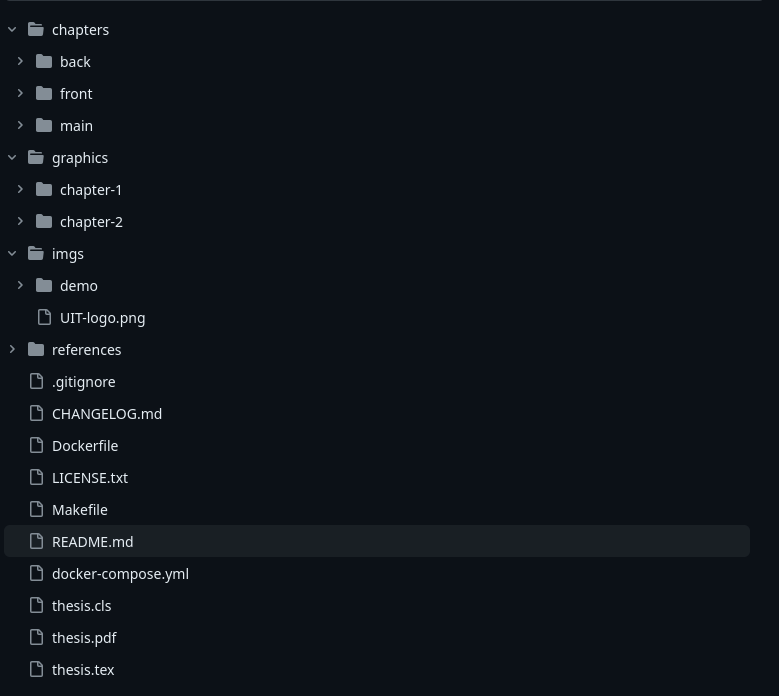
\includegraphics[scale=0.5]{chapter1/chap1-project-directory.png}
%     \caption{Cấu trúc thư mục của dự án}
%     \label{fig:chap1-project-directory}
% \end{figure}


% Thư mục \textbf{\textit{front}} tương ứng với các trang thông tin hội đồng chấm tốt nghiệp, lời cảm ơn, danh mục từ viết tắt... Thư mục \textbf{\textit{main}} chứa các chương của báo cáo. Báo cáo đánh số thứ tự riêng cho phần \textit{\textbf{front}}, trong khi phần các chương chính và phần phụ lục được đánh số giống nhau. Báo cáo đánh số trang bắt đầu từ trang tóm tắt, chữ số Ả-rập, bắt đầu bằng 1.

% Thư mục \textbf{\textit{graphics}} chứa hình ảnh được chèn vào báo cáo. Tương ứng với mỗi chương sẽ có 1 thư mục hình ảnh của chương đó.

% Thư mục \textbf{\textit{imgs}} là thư mục chứa hình ảnh của dự án, nó bao gồm các logo, watermark hoặc hình ảnh phục vụ cho document trên github. Hình chèn vào báo cáo không được lưu trong thư mục này.

% Thư mục \textbf{\textit{references}} chứa các file chỉ mục tài liệu tham khảo. Tương tự như mỗi chapter một file .tex, nó cũng có riêng một file .bib để chỉ rõ các tài liệu tham khảo nào được sử dụng trong chuong nào.

% File \textbf{\textit{thesis.cls}} là file quy định các câu lệnh, mức chỉ mục đánh số hình ảnh, bảng biểu, phần, chương. Quy định header và footer, trang  bìa.... Chi tiết xem trong file. Hãy chắc chắn rằng bạn hiểu rõ tất cả nếu muốn thay đổi gì trong file này.

% File \textbf{\textit{thesis.tex}} là file quy định cấu trúc báo cáo, chương nào trước, chương nào sau, quy định thư mục hình ảnh chèn trong báo cáo. Nó quy định thông tin người báo cáo thông qua các câu lệnh được quy định trong file .cls. 

% \section{Thay đổi các biến khi sử dụng}

% Hai bìa của luận văn được tự động tạo bởi latex. Vì vậy, có các biến được quy định để đảm nhiệm nó. Các biến cần thay đổi được đặt tại thư mục gốc, tập tin \textit{thesis.tex}, được thể hiện trong hình \ref{fig:chap1-information-variable}.

% \begin{figure}
%     \centering
%     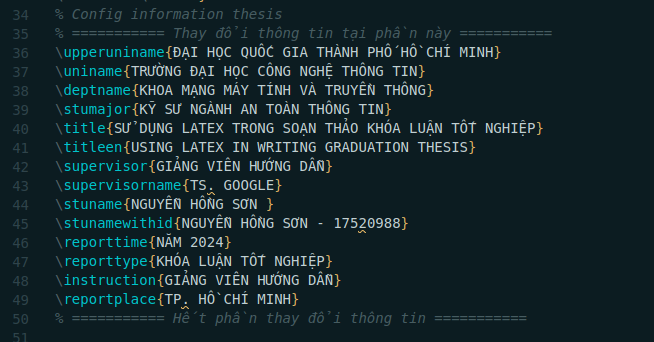
\includegraphics[scale=0.7]{chapter1/chap1-information-variable.png}
%     \caption{Phần thay đổi thông tin trang bìa}
%     \label{fig:chap1-information-variable}
% \end{figure}

% Các phần tiếp theo, quy định các nội dung được thêm vào báo cáo chính. Nếu một tập tin xuất hiện trong thư mục chapters nhưng không được khai báo bằng lệnh \textit{include} thì cũng không xuất hiện trong báo cáo. Vậy nên các chương mới bắt buộc phải được khai báo trong \textit{thesis.tex}. Các phần tài liêu tham khảo cũng được hiểu tương tự.

\chapter{Tổng quan}
\label{chap:chap1}
\section{Bối cảnh và bài toán nghiên cứu}
Trong bối cảnh công nghệ blockchain ngày càng phát triển, nhu cầu về mở rộng \cite{song2024advancing} và cải thiện hiệu suất giao dịch đang ngày càng trở nên cấp thiết  \cite{etherscan_pending} \cite{etherscan_token}. Các giải pháp để cải thiện vấn đề này đã được đề xuất như sharding, side-chains, state-channels,... Trong số đó, ZK-Rollup đã được nghiên cứu và ứng dụng rộng rãi như một giải pháp để cải thiện khả năng mở rộng blockchain bằng layer 2 hiệu quả. Các giải pháp ZK-Rollup đã được triển khai và sử dụng phổ biến trong những năm gần đây như ZKSync Era, Starknet, Polygon zkEVM \cite{chaliasos2024analyzing},... đã cho thấy ZK-Rollup là giải pháp tiềm năng để nghiên cứu, tối ưu và phát triển nhắm đến mục tiêu chính là cải thiện khả năng mở rộng cho các blockchain layer 1 như Ethereum.
ZK-Rollups tổng hợp nhiều giao dịch riêng lẻ ngoài chuỗi thành một lô duy nhất \cite{thibault2022blockchain}. Sau đó, một bằng chứng không tri thức (ZKP - Zero Knowledge Proof) về tính hợp lệ của các giao dịch này được tạo ra, và chỉ có bằng chứng này, cùng với dữ liệu giao dịch đã nén, được đăng tải lên lớp 1 để xác minh. Phương pháp này giảm thiểu đáng kể dữ liệu và tính toán trên chuỗi, từ đó tăng cường thông lượng giao dịch và giảm phí gas. Điều này không chỉ làm tăng tốc độ giao dịch mà còn đảm bảo an toàn bằng cách kế thừa các đảm bảo bảo mật của lớp 1 thông qua các bằng chứng hợp lệ \cite{saif2024survey}.
Mặc dù là giải pháp đầy hứa hẹn, nhưng việc triển khai thực tiễn ZK-Rollup đang gặp phải một số thách thức đáng kể, chủ yếu liên quan đến sự phức tạp cố hữu của các mạch bằng chứng không kiến thức \cite{zhou2024leveraging}. Việc xây dựng các mạch ZK (zero-knowledge) một cách thủ công rất phức tạp và dễ mắc lỗi \cite{chaliasos2024sok}. Hiệu suất của các hệ thống ZKP, đặc biệt là quy trình tạo bằng chứng, hiện đang là một trong những mối quan tâm lớn khi nghiên cứu về bằng chứng không kiến thức. Với các mạch phức tạp, số lượng các ràng buộc trở thành một trong những yếu tố gây cản trở, ảnh hưởng đến nhiều khía cạnh của quy trình tạo bằng chứng, chẳng hạn như thời gian biên dịch mạch, thời gian tạo bằng chứng và mức tiêu thụ bộ nhớ cần thiết để thực hiện những tác vụ này \cite{belles2022circom}.
Mặc dù đã có nhiều nỗ lực nhằm tăng tốc tính toán bằng chứng, những tiến bộ trong việc tối ưu hóa quy trình tạo bằng chứng vẫn còn hạn chế, cản trở đến hiệu suất tổng thể. Các nghiên cứu về chủ đề này thường tập trung vào việc phát triển các hệ thống tạo bằng chứng, đề xuất các hệ thống ZKP mới \cite{gong2022analysis} như STARK \cite{ben2018scalable}, Bulletproof \cite{bunz2018bulletproofs} và Plonk \cite{gabizon2019plonk}. Tuy nhiên, vấn đề thực tiễn đầu tiên mà các nhà phát triển phải đối mặt nằm trong hệ thống ràng buộc và trình biên dịch. Tập trung vào các cờ tối ưu của trình biên dịch Circom, một công cụ quan trọng và phổ biến để quản lý độ phức tạp và hiệu suất của mạch, sẽ trực tiếp giải quyết khoảng trống này ở cấp độ cơ bản của việc thiết kế và triển khai mạch.

Việc hiểu rõ tác động của các cờ tối ưu hóa này sẽ cung cấp kiến thức nền tảng quan trọng, giúp các nhà phát triển đưa ra quyết định tốt hơn ngay từ giai đoạn thiết kế và triển khai mạch, trước khi xem xét các tối ưu hóa phức tạp hơn ở cấp độ hệ thống (như độ trễ mạng, thiết kế hệ thống hoặc các chiến lược tối ưu hệ thống ZKP chuyên sâu hơn) \cite{liang2025sok}.

Nhằm giải quyết những thách thức trên, khoá luận này đề xuất nghiên cứu đề tài ``NÂNG CAO HIỆU SUẤT GIAO DỊCH ERC-20 TRÊN ZK-ROLLUP THÔNG QUA XỬ LÝ RÀNG BUỘC MẠCH GROTH16''. Đề tài này tập trung vào hai mục tiêu chính:
\begin{enumerate}
    \item \textbf{Phân tích sự ảnh hưởng của ràng buộc đến các giai đoạn trong quá trình tạo bằng chứng không kiến thức}: Nghiên cứu định lượng sự ảnh hưởng của số lượng ràng buộc đến thời gian tạo bằng chứng không kiến thức, và sự đánh đổi giữa thời gian biên dịch với số lượng ràng buộc được tối ưu khi áp dụng các cờ tối ưu của Circom.
    \item \textbf{Cung cấp khung gợi ý sử dụng cờ tối ưu hoá Circom}: Đề xuất một khung gợi ý để sử dụng các cờ tối ưu hoá Circom trong thực tế nhằm cân bằng thời gian biên dịch mạch và hiệu suất tạo bằng chứng không kiến thức trong quá trình phát triển mạch không kiến thức.
\end{enumerate}
Với những mục tiêu được đề cập ở trên, khoá luận này hy vọng sẽ cung cấp được một cái nhìn cụ thể, trực quan hơn về cách Circom tối ưu hoá ràng buộc của mạch nhằm tăng hiệu suất tạo bằng chứng không kiến thức. Đồng thời hỗ trợ giải quyết nhu cầu thực tế trong phát triển hệ thống ZK-Rollup. Việc quản lý tối ưu hóa ràng buộc một cách hiệu quả không chỉ giảm thiểu chi phí tạo bằng chứng mà còn ảnh hưởng trực tiếp đến chu kỳ lặp khi phát triển ứng dụng, tạo điều kiện thuận lợi cho việc tích hợp các mạch không kiến thức vào các ứng dụng blockchain. Qua đó, hỗ trợ việc áp dụng rộng rãi ZK-Rollup trong các môi trường blockchain nhạy cảm về chi phí và yêu cầu cao về hiệu suất.

\section{Mục tiêu}

Công nghệ bằng chứng không kiến thức khi được áp dụng vào các ứng dụng thực tế như ZK-Rollup luôn gặp phải vấn đề cố hữu là kích thước mạch lớn và thời gian tạo bằng chứng dài do các hoạt động mật mã phức tạp trong các thuật toán đại số. Do đó, khoá luận này sẽ tập trung nghiên cứu vào tác động của ràng buộc đến thời gian tạo bằng chứng không kiến thức, cũng như những đánh đổi về thời gian biên dịch để tối ưu mạch chứng minh không kiến thức nhằm giảm số lượng ràng buộc. Từ đó đưa ra một khung gợi ý sử dụng cờ tối ưu hoá Circom nhằm tăng hiệu quả phát triển ứng dụng sử dụng bằng chứng không kiến thức như ZK-Rollup trong thực tế. 
Cụ thể, khoá luận này đề ra các mục tiêu cụ thể như sau:
\begin{enumerate}
    \item \textbf{Khảo sát và phân tích các phương pháp hiện tại}: Bắt đầu quá trình nghiên cứu, khoá luận sẽ tiến hành một khảo sát toàn diện về những phương pháp giúp cải tiến hiệu suất tạo bằng chứng không kiến thức cho hệ thống zk-SNARKs. Từ đó thu hẹp phạm vi lại hướng đến việc cải thiện hiệu suất tạo bằng chứng không kiến thức thông qua tối ưu hoá ràng buộc trong mạch. Mục tiêu của giai đoạn này là tìm hiểu về các giải pháp tối ưu cho việc tạo bằng chứng không kiến thức, tìm ra khoảng trống nghiên cứu nhằm nghiên cứu đưa ra cách giải quyết hiệu quả cho khoảng trống này (ví dụ các công trình như
    \cite{albert2022distilling, ben2018scalable, bunz2018bulletproofs, ernstberger2024zk,gabizon2019plonk,gong2022analysis, el2024evaluating,  pailoor2023automated}).
    \item \textbf{Phân tích và đánh giá định lượng tác động của các cờ tối ưu hóa ràng buộc khác nhau (--O0, --O1, --O2) trong trình biên dịch Circom đối với hiệu suất của hệ thống ZK-Rollup mô phỏng giao dịch ERC-20}: Tiếp theo, khoá luận sẽ tập trung vào việc phân tích các dữ liệu lấy được từ quá trình thực nghiệm. Quá trình này bao gồm việc đo lường và so sánh:
    \begin{itemize}
        \item Số lượng ràng buộc tổng thể, số lượng ràng buộc tuyến tính và phi tuyến được tạo ra.
        \item Thời gian cần thiết để biên dịch mạch (compilation time).
        \item Thời gian cần thiết để tạo bằng chứng không tri thức (proving time) sử dụng backend Groth16.
        \item Thời gian và chi phí để xác minh bằng chứng không kiến thức trên blockchain lớp 1.
    \end{itemize}
    \item \textbf{Khảo sát mối quan hệ giữa các mức tối ưu hóa ràng buộc, kích thước lô giao dịch, và các chỉ số hiệu suất đã nêu}: Xác định các xu hướng và sự đánh đổi giữa thời gian biên dịch và thời gian tạo bằng chứng khi thay đổi các cờ tối ưu khác nhau.

    \item \textbf{Phân tích cơ chế hoạt động của cờ tối ưu hóa --O2 trong Circom, đặc biệt là cách nó loại bỏ các ràng buộc tuyến tính và ảnh hưởng đến cấu trúc ràng buộc phi tuyến còn lại}: Đánh giá hiệu quả của việc tập trung tài nguyên tính toán vào các ràng buộc phi tuyến.

    \item \textbf{Đề xuất một khung hướng dẫn thực tiễn cho việc lựa chọn cờ tối ưu hóa Circom phù hợp}:  Khung này sẽ dựa trên các kết quả thực nghiệm và xem xét các yếu tố như giai đoạn phát triển của dự án (phát triển, kiểm thử, sản xuất), tần suất cập nhật mạch, và khối lượng bằng chứng dự kiến cần tạo. Góp phần vào việc giảm thiểu chi phí triển khai, rút ngắn chu kỳ phát triển, và thúc đẩy việc áp dụng rộng rãi công nghệ ZK-Rollup trong các ứng dụng blockchain thực tế.
\end{enumerate}
\section{Phạm vi đề tài và đối tượng nghiên cứu}
Đề tài sẽ tập trung phân tích mức độ hiệu quả cũng như các đánh đổi khi áp dụng các mức tối ưu hoá ràng buộc mạch của Circom. Từ đó đánh giá sự ảnh hưởng của các thông số ghi lại được trong quá trình tạo bằng chứng không kiến thức và đề xuất khung hướng dẫn sử dụng cờ tối ưu Circom phù hợp với từng giai đoạn phát triển mạch bằng chứng không kiến thức trong ZK-Rollup thực tế.
Đối tượng nghiên cứu của đề tài bao gồm:

\begin{itemize}
    \item \textbf{Hệ thống ZK-Rollup}: Tập trung vào triển khai thực nghiệm với hệ thống ZK-Rollup mô phỏng với tác vụ chính là giao dịch token ERC-20.
    \item \textbf{Công cụ và cơ chế tối ưu hoá ràng buộc cho mạch chứng minh không kiến thức}: Phạm vi nghiên cứu được giới hạn trong việc phân tích và đánh giá tác động của các cờ tối ưu hóa ràng buộc (-O0, -O1, và -O2) của trình biên dịch Circom.
    \item \textbf{Hệ thống chứng minh không kiến thức}: Các thí nghiệm và phân tích sẽ được thực hiện dựa trên hệ thống bằng chứng không kiến thức Groth16, một trong những hệ thống zk-SNARK phổ biến nhất hiện nay.
    \item \textbf{Giải pháp sử dụng các mức tối ưu hoá hiệu quả}: Đưa ra khung gợi ý sử dụng các mức tối ưu hoá phù hợp khi phát triển mạch bằng chứng không kiến thức khi xây dựng ZK-Rollup.
\end{itemize}

\section{Cấu trúc báo cáo khoá luận}
Khoá luận này có cấu trúc gồm 6 chương, được trình bày như sau: 
\begin{itemize}
    \item \textbf{Chương \ref{chap:chap1} - Tổng quan:} Trình bày bối cảnh, mục đích, đối tượng và phạm vi nghiên cứu của đề tài.
    \item \textbf{Chương \ref{chap:chap2} - Nghiên cứu liên quan:} Trình bày các công trình nghiên cứu liên quan và khoảng trống nghiên cứu.
    \item \textbf{Chương \ref{chap:chap3} - Cơ sở lý thuyết:} Cung cấp kiến thức về blockchain, ZK-Rollup, giao dịch ERC-20, kiến thức liên quan về hệ thống chứng minh không kiến thức được sử dụng, trình biên dịch Circom và các cờ tối ưu hoá.
    \item \textbf{Chương \ref{chap:chap4} - Phương pháp đề xuất và công cụ hỗ trợ:} Trình bày chiến lược tối ưu hoá ràng buộc theo vòng đời phát triển mạch ZKP sử dụng Circom, gọi tắt là ZCLS (ZK Circuit Lifecycle Strategy), cùng các bước thực nghiệm và công cụ CirMetrics được thiết kế để hỗ trợ triển khai chiến lược này.
    \item \textbf{Chương \ref{chap:chap5} - Kết quả thực nghiệm và đánh giá:} Trình bày kết quả thực nghiệm, thảo luận và đề xuất khung gợi ý sử dụng cờ tối ưu của trình biên dịch Circom.
    % \item \textbf{Chương \ref{chap:chap6}} - \textbf{CirMetrics:} Giới thiệu hệ thống hỗ trợ theo dõi các thống số của mạch ZK, hỗ trợ các nhà phát triển quản lí mạch trong quá trình xây dựng mạch ZK.
    \item \textbf{Chương \ref{chap:chap6} - Kết luận và hướng phát triển:} Trình bày những kết quả đạt được, những đóng góp và đề xuất mới. 
    \item \textbf{Tài liệu tham khảo:} Các công trình nghiên cứu được trích dẫn trong khoá luận.
\end{itemize}
\chapter{Các công trình nghiên cứu liên quan}
\label{chap:chap2}

Các nghiên cứu gần đây về việc tối ưu hóa hiệu suất tạo bằng chứng không kiến thức (ZKP), đặc biệt liên quan đến zk-SNARKs, có thể được phân loại chung thành hai hướng chính: tối ưu hóa ở phía back-end (hệ thống bằng chứng) và tối ưu hóa ở phía front-end (hệ thống ràng buộc/mạch để tạo bằng chứng) \cite{ernstberger2024zk} như minh hoạ ở hình \ref{fig:chapter2-SNARKs_realworld}.

% \begin{figure}[H]
%     \centering
%     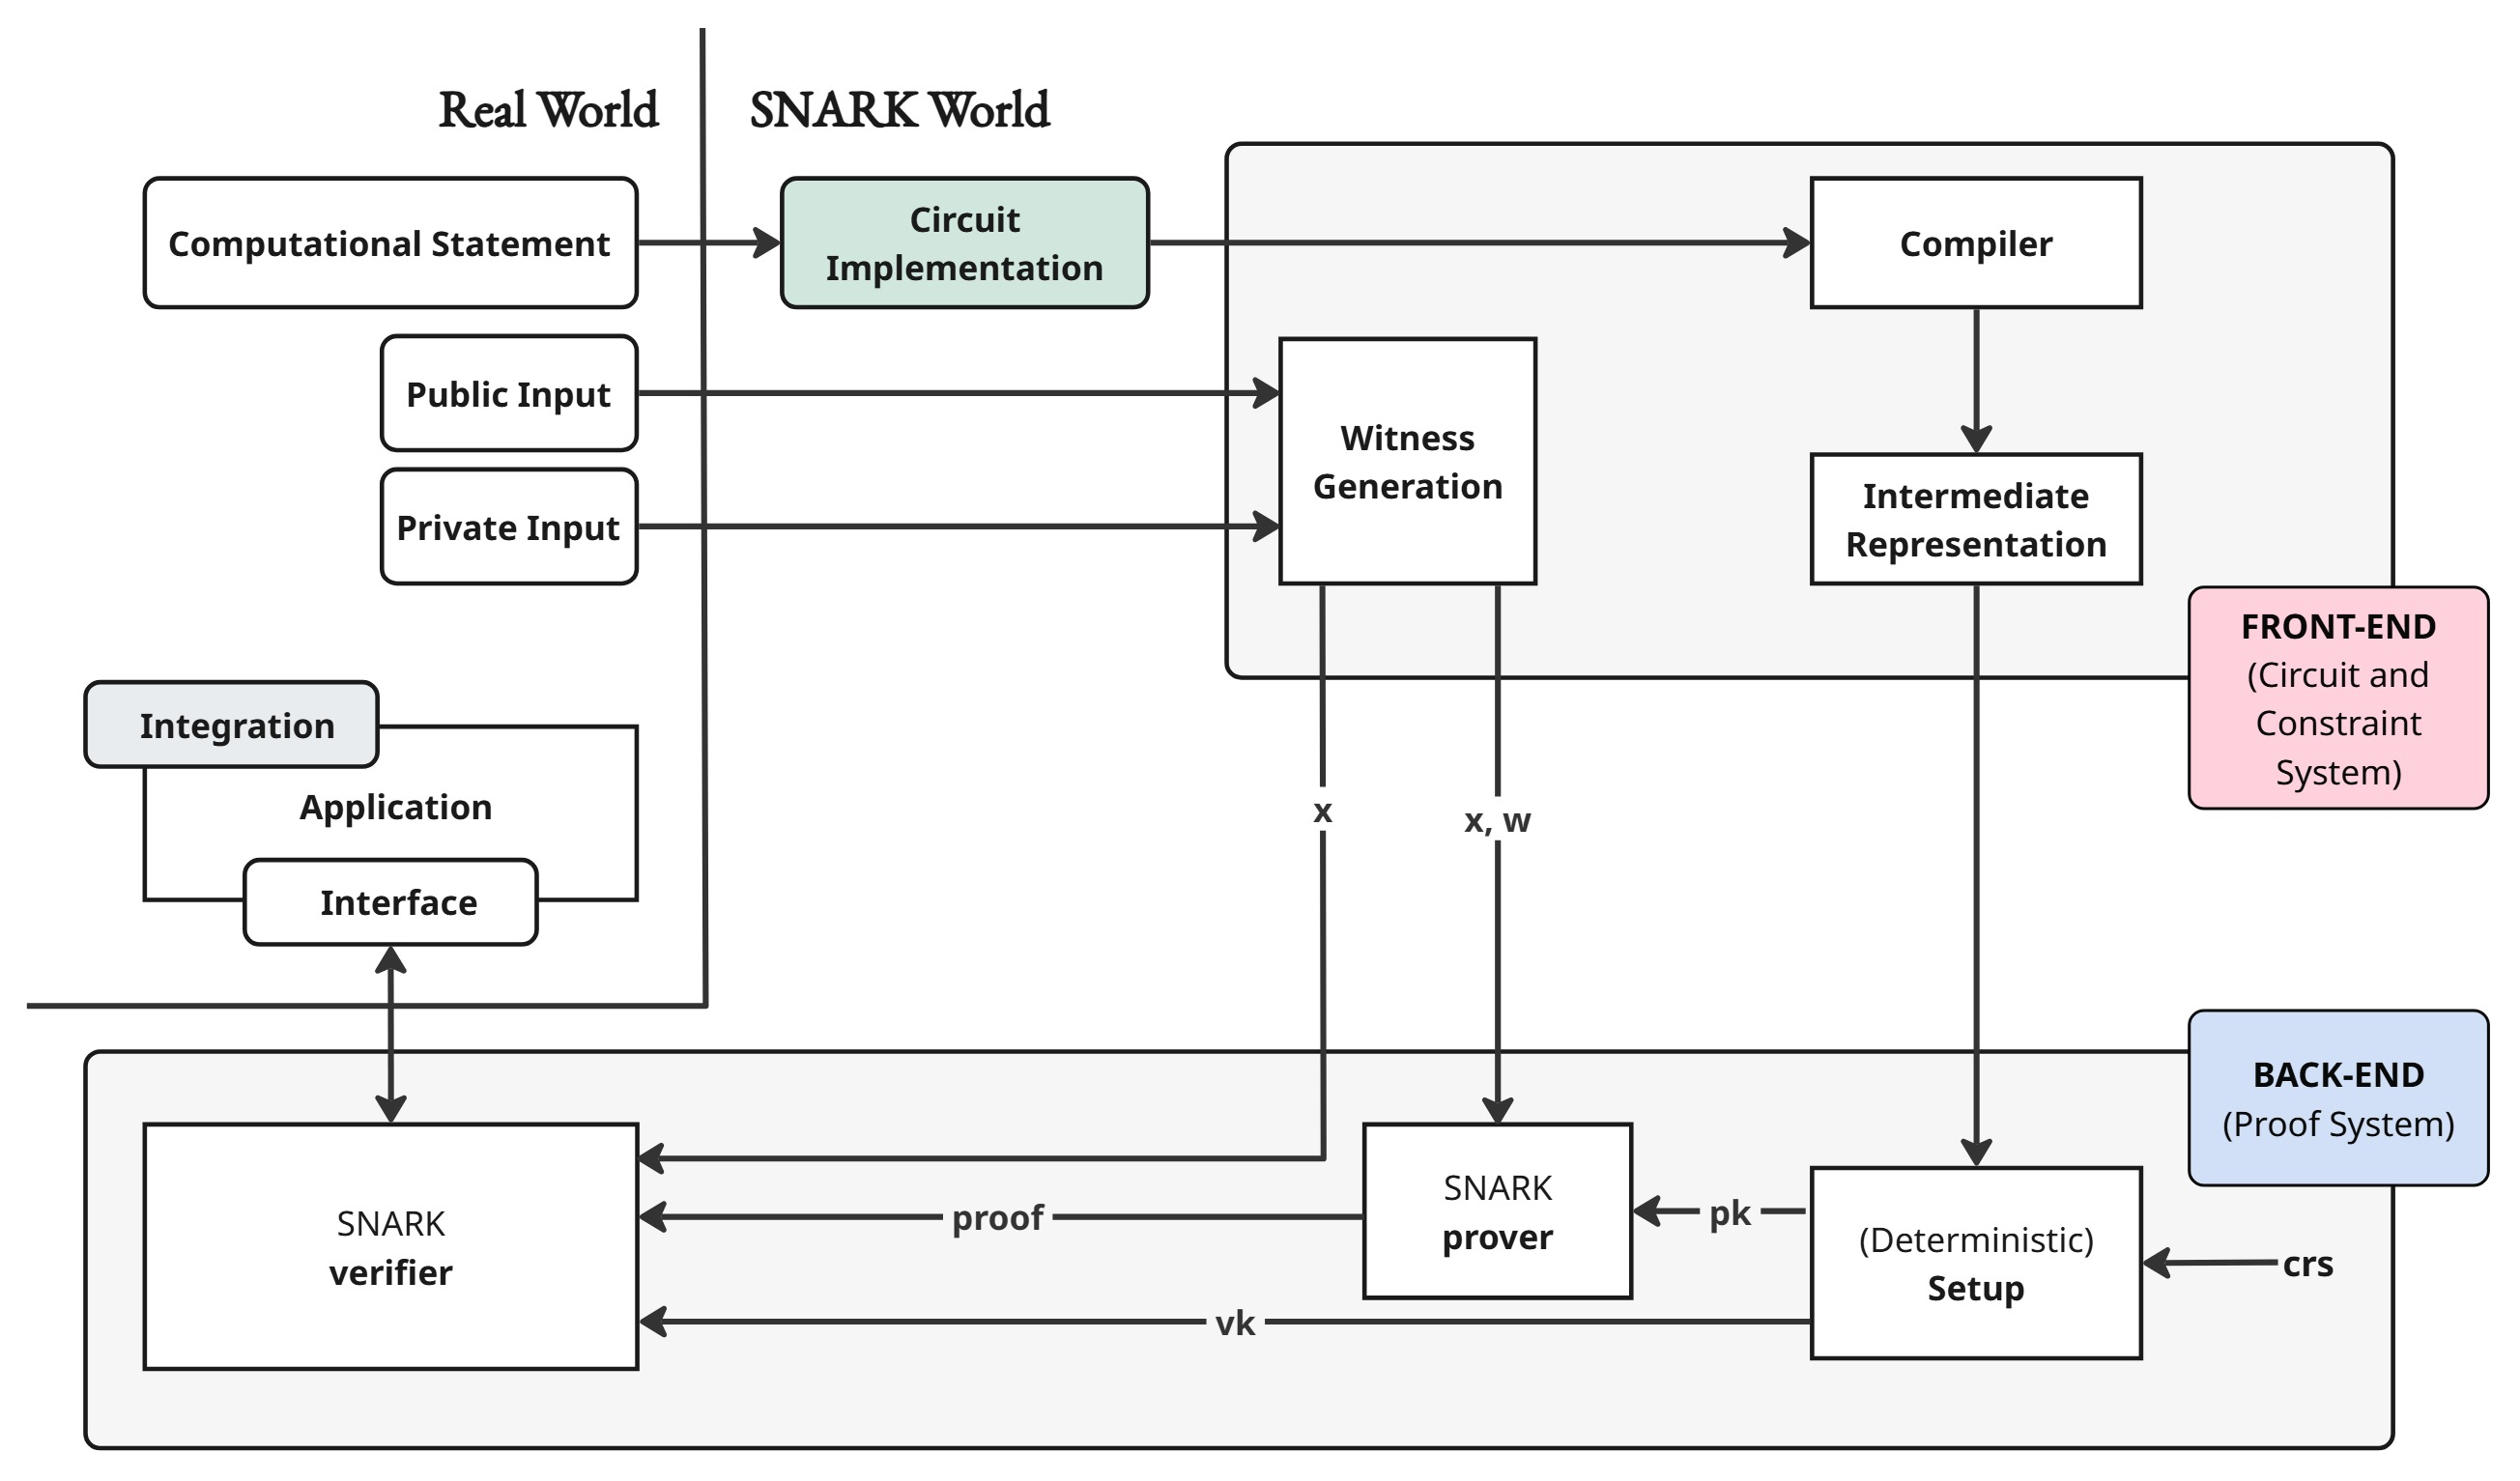
\includegraphics[width = 0.9\textwidth]{imgs/SNARKs_realworld.jpg}
%     \caption{Mối quan hệ giữa front-end, back-end của hệ thống zk-SNARKs và ứng dụng sử dụng hệ thống này}
%     \label{fig:chapter2-SNARKs_realworld}
% \end{figure}

\begin{figure}[H]
    \centering
    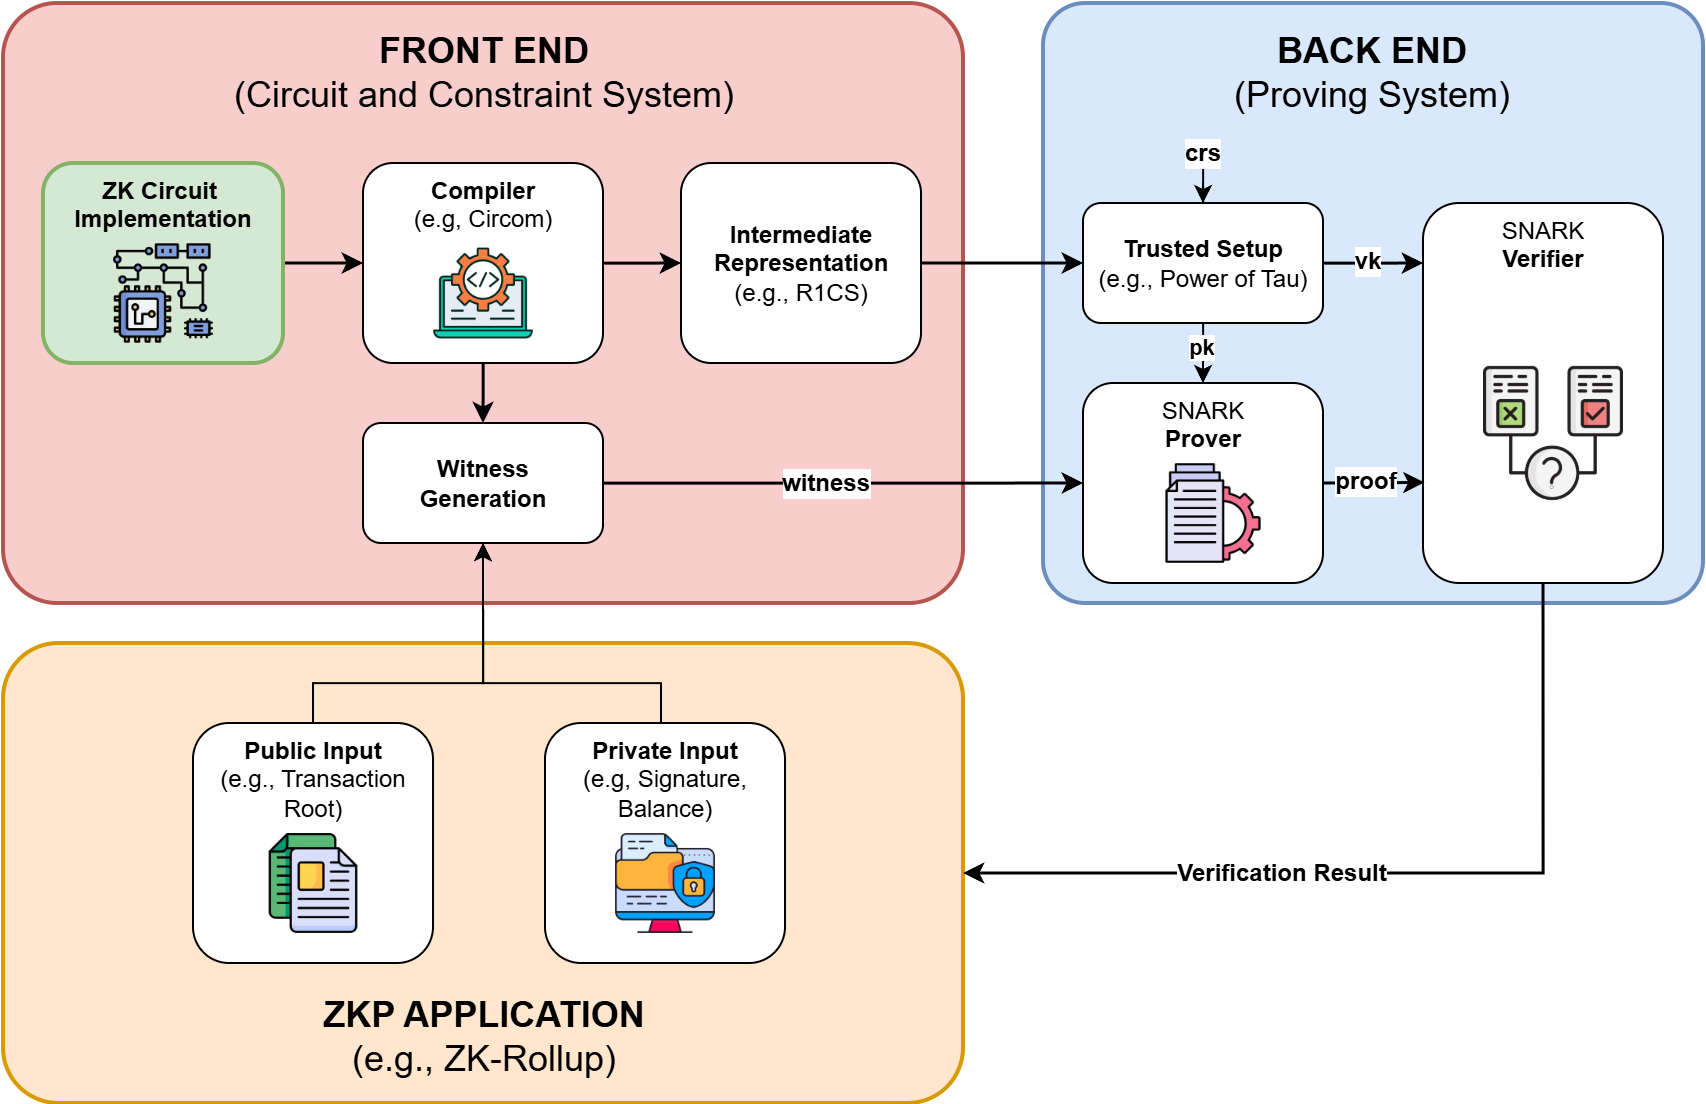
\includegraphics[width = 0.9\textwidth]{imgs/SNARKsFlow.png}
    \caption{Mối quan hệ giữa front-end, back-end của hệ thống zk-SNARKs và ứng dụng sử dụng hệ thống này}
    \label{fig:chapter2-SNARKs_realworld}
\end{figure}

\section{Tối ưu hóa back-end}
% Các nỗ lực trong lĩnh vực này tập trung vào việc đề xuất các sơ đồ ZKP mới và hiệu quả. GENES \cite{liu2025genes} là một zk-SNARK đệ quy không yêu cầu thiết lập tin cậy, giải quyết các vấn đề về thời gian tạo và xác minh bằng chứng trong các ứng dụng blockchain. Nó kết hợp nhiều phiên bản của Hệ thống Ràng buộc Bậc 1 (R1CS) thành một và sử dụng các "trợ lý" để phân phối áp lực tính toán, đạt được thời gian xác minh không đổi O(1), mặc dù kích thước bằng chứng lớn hơn so với các sơ đồ khác. HyperPlonk \cite{chen2023hyperplonk}, được phát triển dựa trên Plonk, sử dụng cấu trúc dữ liệu hypercube Boolean và cam kết đa thức đa tuyến để nâng cao hiệu suất, loại bỏ nhu cầu về các phép toán FFT phức tạp và giảm thời gian tạo bằng chứng.

% Hơn nữa, các biến thể của các sơ đồ hiện có, chẳng hạn như Groth16, đã được đề xuất để cải thiện hiệu suất. Polymath \cite{lipmaa2024polymath}, một zk-SNARK được thiết kế cho hệ thống ràng buộc Lập trình Số học Bậc 2 (SAP) thay vì R1CS của Groth16, sử dụng các sơ đồ cam kết đa thức KZG để đạt được kích thước bằng chứng ngắn hơn, đặc biệt ở các mức độ bảo mật cao hơn. Những tiến bộ này nhằm giảm thời gian tạo bằng chứng, kích thước bằng chứng và thời gian xác minh, hoặc loại bỏ nhu cầu về thiết lập tin cậy.

Những nỗ lực trong lĩnh vực này tập trung vào việc đề xuất các sơ đồ ZKP mới và hiệu quả hơn, chẳng hạn như GENES \cite{liu2025genes} -- một zk-SNARK đệ quy mới không yêu cầu thiết lập tin cậy, được thiết kế để giải quyết các vấn đề về thời gian sinh và xác minh bằng chứng trong các ứng dụng ZKP, đặc biệt là trên blockchain. GENES kết hợp các bằng chứng đệ quy, hợp nhất nhiều phiên bản của hệ thống ràng buộc bậc 1 (R1CS -- Rank 1 Constraint System) \cite{ben2013snarks} thành một, và phân bổ việc tính toán bằng cách sử dụng các ``trợ lý'' để phân tán các cam kết chứng minh. Sơ đồ ZKP này nổi bật với thời gian xác minh không đổi \(O(1)\), mặc dù có nhược điểm là kích thước bằng chứng lớn hơn so với các sơ đồ khác. 

HyperPlonk \cite{chen2023hyperplonk} là một hệ thống bằng chứng mới được phát triển dựa trên Plonk, sử dụng một cấu trúc dữ liệu đặc biệt gọi là hypercube boolean và áp dụng kỹ thuật cam kết đa thức gọi là cam kết đa thức đa tuyến để nâng cao hiệu quả. So với Plonk truyền thống, HyperPlonk mang lại một số lợi ích: loại bỏ nhu cầu tính toán FFT (Fast Fourier Transform) phức tạp và xử lý các ``cổng'' (phép toán) tùy chỉnh với độ phức tạp cao hơn một cách hiệu quả hơn. Những cải tiến này giảm đáng kể thời gian cần thiết để sinh bằng chứng. 
Bên cạnh đó, đã có nhiều nghiên cứu nhằm nâng cao các sơ đồ ZKP hiện có, chẳng hạn như Groth16, với các biến thể như Polymath \cite{lipmaa2024polymath} - một zk-SNARK được thiết kế cho hệ thống ràng buộc ``Lập Trình Số Học Bình Phương'' (SAP -- Square Arithmetic Programming) thay vì R1CS của Groth16, sử dụng các sơ đồ cam kết đa thức KZG (Kate-Zaverucha-Goldberg Polynomial Commitments). Mục tiêu chính của nó là đạt được kích thước bằng chứng ngắn hơn đáng kể, đặc biệt ở các mức độ bảo mật cao hơn. 
Mục tiêu tổng thể của những phương pháp này là giảm thời gian sinh bằng chứng, kích thước bằng chứng và thời gian xác minh, hoặc loại bỏ nhu cầu thiết lập tin cậy.

\section{Tối ưu hóa front-end}
\subsection{Tối ưu hoá về độ an toàn của mạch ZK}
% Nghiên cứu về việc tối ưu hóa các ràng buộc cho các mạch ZK đã thu hút được sự chú ý đáng kể, chủ yếu tập trung vào các khía cạnh bảo mật và tính chính xác của mạch. Điều này bao gồm việc giải quyết các mạch bị ràng buộc không đủ, chấp nhận các nhân chứng không hợp lệ, dẫn đến các lỗ hổng như khai thác trong zkSync \cite{tang2024zero}, cũng như các mạch bị ràng buộc quá mức, từ chối các nhân chứng hợp lệ, ảnh hưởng đến tính toàn vẹn của hệ thống. Các nghiên cứu đáng chú ý bao gồm AC$^4$ \cite{chen2024ac4}, một công cụ mô hình hóa các mạch Circom như các hệ thống đa thức để phát hiện các vấn đề ràng buộc, và QED$^2$ (Picus) \cite{pailoor2023automated}, kết hợp lý luận ràng buộc duy nhất nhẹ (UCP) với các bộ giải SMT để xác định các mạch bị ràng buộc không đủ. Circomspect \cite{circomspect2022}, một công cụ phân tích tĩnh, và Coda của Veridise \cite{liu2024certifying}, sử dụng xác minh chính thức, cũng đóng góp vào việc cải thiện bảo mật và tính chính xác của mạch.

% Ngoài ra, tối ưu hóa ràng buộc đã được khám phá trong các nghiên cứu như của Albert et al. \cite{albert2022distilling}, tập trung vào việc loại bỏ các ràng buộc dư thừa từ R1CS bằng cách sử dụng các hệ thống biến đổi dựa trên quy tắc và kỹ thuật loại bỏ Gaussian. Những phương pháp này nhằm giảm chi phí tính toán trong việc tạo ZKP bằng cách tối thiểu hóa các ràng buộc không cần thiết.

% Mặc dù đã có các nghiên cứu hiện có về tối ưu hóa ở phía front-end, các nghiên cứu này thường nhấn mạnh vào tính chính xác của mạch hoặc các kỹ thuật tối ưu hóa trình biên dịch tổng quát, vẫn còn một khoảng trống đáng kể trong phân tích thực nghiệm định lượng liên quan đến tác động của các tùy chọn tối ưu hóa trình biên dịch, chẳng hạn như các cờ trong Circom, đến các chỉ số hiệu suất như thời gian biên dịch và thời gian tạo bằng chứng trong các ứng dụng zk-rollup phức tạp ERC-20. Nghiên cứu của chúng tôi giải quyết khoảng trống này bằng cách định lượng các sự đánh đổi về hiệu suất và làm rõ cơ chế của tối ưu hóa --O2, nhằm giảm tổng số ràng buộc trong các phép toán mật mã cốt lõi cho các giao dịch ERC-20. Chúng tôi đề xuất một khung tối ưu hóa mạch, được hỗ trợ bởi dữ liệu thực nghiệm, để cung cấp hướng dẫn thực tiễn cho việc cải thiện hiệu suất zk-rollup thông qua quản lý ràng buộc hiệu quả. 

Nghiên cứu liên quan đến tối ưu hóa các ràng buộc cho các mạch ZK (Zero-knowledge) cũng đã thu hút nhiều sự chú ý. Tuy nhiên, hầu hết các công trình này chủ yếu tập trung vào các khía cạnh bảo mật, giải quyết các vấn đề liên quan đến tính chính xác của mạch. Điều này bao gồm việc xác định và khắc phục các vấn đề liên quan đến mạch thiếu ràng buộc (mạch chấp nhận các chứng cứ không hợp lệ, dẫn đến các lỗ hổng bảo mật nghiêm trọng, chẳng hạn như khai thác trong zkSync cho phép đánh cắp tài sản \cite{tang2024zero}) và mạch thừa ràng buộc (mạch từ chối các chứng cứ hợp lệ, ảnh hưởng đến tính hoàn chỉnh của hệ thống). Các nghiên cứu nổi bật giải quyết các vấn đề này bao gồm AC$^4$ \cite{chen2024ac4}—một công cụ mô hình hóa mạch Circom dưới dạng hệ thống đa thức và áp dụng các thuật toán đại số để kiểm tra các vấn đề thừa hoặc thiếu ràng buộc; QED$^2$ (Picus) \cite{pailoor2023automated}—một kỹ thuật và công cụ tự động được thiết kế để phát hiện các mạch ZKP thiếu ràng buộc bằng cách kết hợp lý luận ràng buộc duy nhất nhẹ (lightweight UCP -- unique constraint propagation) với các bộ giải lý thuyết module về tính thỏa được (SMT -- Satisfiability Modulo Theories); Circomspect \cite{circomspect2022}—một công cụ phân tích tĩnh (kiểm tra mã nguồn của các mạch mà không cần thực thi mã) để phân tích và xác định các lỗ hổng bảo mật trong các mạch ZKP; và Coda của Veridise \cite{liu2024certifying}—một công cụ sử dụng xác minh chính thức để kiểm tra các thuộc tính và tính chính xác của các mạch ZKP.

\subsection{Tối ưu hoá nhằm tinh gọn ràng buộc trong mạch ZK}
Ở khía cạnh tối ưu hoá hệ thống ràng buộc để gia tăng hiệu suất tạo bằng chứng ZKP, các công trình này sẽ tập trung vào việc tinh gọn, giảm thiểu số lượng ràng buộc trong các mạch ZK nhằm cải thiện khả năng tạo bằng chứng. Chẳng hạn như công trình của Albert et al. \cite{albert2022distilling}, tập trung vào việc tinh gọn các ràng buộc từ R1CS bằng cách loại bỏ các phần ràng buộc không ảnh hưởng đến bảo mật. Cụ thể, họ nhằm mục tiêu xác định và loại bỏ các ràng buộc dư thừa bằng cách sử dụng một khung cho việc giảm R1CS dựa trên hệ thống biến đổi có quy tắc và một kỹ thuật tối ưu hóa ràng buộc mới dựa trên phương pháp khử Gaussian để suy ra các ràng buộc tuyến tính từ các ràng buộc phi tuyến, với mục tiêu giảm lượng ràng buộc dư thừa trong mạch R1CS, từ đó giảm chi phí sinh bằng chứng không kiến thức. Công trình nghiên cứu này cũng đề cập rằng đây là công trình đầu tiên nghiên cứu các kỹ thuật áp dụng trên ràng buộc như một phương pháp chính thức (formal method) để giải quyết các thách thức trong việc phân tích và tối ưu hóa các giao thức ZK.

Có thể thấy rằng, mặc dù có sự tồn tại của các nghiên cứu về tối ưu hóa ở phía front-end, các nghiên cứu này thường tập trung vào tính chính xác của mạch (bảo mật). Một khoảng trống đáng kể còn tồn tại trong các nghiên cứu để tinh gọn ràng buộc tương tự như công trình của Albert et al. \cite{albert2022distilling}, nhằm mục đích gia tăng hiệu suất tạo ZKP, và cũng thiếu các cung cấp phân tích thực nghiệm định lượng về tác động của các tùy chọn tối ưu hóa biên dịch (chẳng hạn như các cờ trong Circom) lên các chỉ số hiệu suất (thời gian biên dịch và thời gian sinh bằng chứng) trong bối cảnh các ứng dụng ZK-Rollup ERC-20 phức tạp.

Nghiên cứu của khoá luận này có mục tiêu lấp đầy khoảng trống này bằng cách định lượng các đánh đổi về hiệu suất và làm rõ cơ chế tối ưu hóa --O2, tập trung vào việc giảm tổng số ràng buộc trong các phép toán mật mã cốt lõi của ZK-Rollup cho các giao dịch ERC-20. Từ đó, khoá luận đề xuất một khung tối ưu hóa mạch, hỗ trợ bởi dữ liệu thực nghiệm, để cung cấp hướng dẫn thực tiễn cho việc cải thiện hiệu suất của ZK-Rollup thông qua quản lý ràng buộc hiệu quả. Bảng \ref{tab:related_work_contributions} tóm tắt các công trình liên quan chính và xác định đóng góp của nghiên cứu trong việc tối ưu hóa các mạch ZK nhằm nâng cao hiệu suất cho ứng dụng ZKP.

\begin{table}[h]
    \centering
    \begin{tabularx}{\textwidth}{|c|>{\centering\arraybackslash}X|>{\centering\arraybackslash}X|>{\centering\arraybackslash}X|>{\centering\arraybackslash}X|>{\centering\arraybackslash}X|}
        \hline
        \textbf{Nghiên cứu} & \textbf{Cải thiện hoặc đề xuất hệ thống ZKP mới} &
        \textbf{Đảm bảo an toàn cho các mạch chứng minh không kiến thức} & \textbf{Đơn giản hoá ràng buộc cho mạch chứng minh không kiến thức} & \textbf{Phân tích đánh đổi hiệu suất khi tối ưu hoá mạch} & \textbf{Đề xuất khung tối ưu hoá mạch} \\ 
        \hline
        GENES \cite{liu2025genes} & x &  &  &  &  \\ \hline
        HyperPlonk \cite{chen2023hyperplonk} & x &  &  &  &  \\ \hline
        Polymath \cite{lipmaa2024polymath} & x &  &  &  &  \\ \hline
        AC$^4$ \cite{chen2024ac4} &  & x &  &  &  \\ \hline
        QED$^2$ (Picus) \cite{pailoor2023automated} &  & x &  &  &  \\ \hline
        Circomspect \cite{circomspect2022} &  & x &  &  &  \\ \hline
        Veridise’s Coda \cite{liu2024certifying} &  & x &  &  &  \\ \hline
        Albert et al. \cite{albert2022distilling} &  &  & x &  &  \\ \hline
        Khoá luận này &  &  & x & x & x \\
        \hline
    \end{tabularx}
    \caption{So sánh đóng góp của các công trình nghiên cứu liên quan cùng khoá luận này}
    \label{tab:related_work_contributions}
\end{table}


\chapter{Cơ sở lý thuyết}
\label{chap:chap3}
Chương này sẽ cung cấp nền tảng cơ sở lí thuyết cho đề tài với các nội dung sau:
\begin{itemize}
    \item Công nghệ Blockchain và Ethereum
    \item Giải pháp ZK-Rollup và token ERC-20
    \item zk-SNARKs và Groth16
    \item Trình biên dịch Circom và các mức tối ưu hoá ràng buộc
    \item Phân tích mức tối ưu hoá --O2
\end{itemize}
\section{Công nghệ Blockchain và Ethereum}
\subsection{Khái niệm}
Blockchain là một công nghệ sổ cái phân tán (Distributed Ledger Technology -- DLT) cho phép ghi chép thông tin các giao dịch một cách an toàn, minh bạch và bất biến. Thay vì lưu trữ dữ liệu tập trung trên một máy chủ duy nhất, blockchain phân tán các bản sao của sổ cái trên một mạng lưới các máy tính (node). Mỗi bản ghi giao dịch sẽ được gom lại thành các ``khối'' (blocks), và các khối này được liên kết với nhau theo trình tự thời gian bằng mã hash, tạo thành một ``chuỗi'' liên tục. Khi một khối mới được thêm vào chuỗi, nó không thể bị thay đổi hoặc xóa bỏ, giúp bảo đảm tính toàn vẹn và bất biến của dữ liệu.
\subsection{Kiến trúc blockchain}
Kiến trúc của một blockchain gồm nhiều thành phần kết hợp với nhau để duy trì tính toàn vẹn và chức năng của hệ thống:

\begin{itemize}
    \item \textbf{Khối (Block)}: Blockchain hoạt động trên một mạng lưới phi tập trung, nơi mỗi nút mạng (node) duy trì một bản sao của toàn bộ sổ cái. Các nút này giao tiếp trực tiếp với nhau để xác minh và lan truyền thông tin các giao dịch và khối mới.
    \item \textbf{Mạng ngang hàng (Peer-to-Peer Network)}: Blockchain hoạt động trên một mạng lưới phi tập trung, nơi mỗi nút mạng (node) duy trì một bản sao của toàn bộ sổ cái. Các nút này giao tiếp trực tiếp với nhau để xác minh và truyền bá các giao dịch và khối mới.
    \item \textbf{Thuật toán đồng thuận (Consensus Mechanism)}:Để đảm bảo tất cả các nút mạng đều có cùng một bản sao của sổ cái và đồng ý về trạng thái của mạng, blockchain sử dụng các thuật toán đồng thuận. Các thuật toán phổ biến bao gồm Proof of Work (PoW) được sử dụng trong Bitcoin và Ethereum 1.0, hoặc Proof of Stake (PoS) được sử dụng trong Ethereum 2.0 và nhiều blockchain hiện đại khác.
    \item \textbf{Mật mã học (Cryptography)}:Mật mã học là nền tảng của blockchain, giúp đảm bảo tính bảo mật và toàn vẹn của dữ liệu. Các kỹ thuật như hàm băm mật mã (cryptographic hash functions) được sử dụng để liên kết các khối và chữ ký số (digital signatures) dùng để xác thực giao dịch và quyền sở hữu tài sản.
    \item \textbf{Sổ cái phân tán (Distributed Ledger)}:Là cơ sở dữ liệu chung được chia sẻ và đồng bộ hóa trên tất cả các nút mạng. Mọi giao dịch được ghi lại trên sổ cái này và có thể được kiểm tra bởi bất kỳ ai trong mạng.
\end{itemize}

\subsection{Cách hoạt động của blockchain}
Quá trình hoạt động cơ bản của một blockchain diễn ra như sau:
\begin{enumerate}
    \item \textbf{Khởi Tạo Giao Dịch:} Một người dùng tạo một giao dịch và ký số bằng khóa riêng của mình.

    \item \textbf{Truyền Bá Giao Dịch:} Giao dịch đã ký được lan truyền đến mạng lưới các nút mạng.

    \item \textbf{Xác Thực Giao Dịch:} Các nút mạng trong mạng lưới nhận giao dịch và xác minh tính hợp lệ của giao dịch này.

    \item \textbf{Tạo Khối:} Các giao dịch hợp lệ được tập hợp lại thành một khối mới.

    \item \textbf{Đồng Thuận:} Khi một nút tìm thấy một khối hợp lệ, nó sẽ lan truyền thông tin khối đó đến các nút khác trong mạng. Các nút khác xác minh khối này và nếu hợp lệ, các nút này sẽ thêm nó vào bản sao sổ cái của mình.

    \item \textbf{Liên Kết Chuỗi:} Khối mới được thêm vào chuỗi các khối hiện có, tạo thành một bản ghi bất biến của tất cả các giao dịch.
\end{enumerate}
\subsection{Các Tính Chất của Blockchain}

Blockchain sở hữu một số tính chất cốt lõi mang lại giá trị riêng của công nghệ này:

\begin{itemize}
    \item \textbf{Phi Tập Trung (Decentralization):} Không có một thực thể trung gian hay cơ quan quản lý duy nhất nào kiểm soát mạng lưới. Quyền lực và dữ liệu được phân tán trên toàn bộ các nút mạng.
    
    \item \textbf{Bất Biến (Immutability):} Một khi giao dịch đã được ghi vào một khối và khối đó đã được thêm vào chuỗi, nó không thể bị thay đổi hoặc xóa bỏ. Điều này đảm bảo tính toàn vẹn lịch sử của dữ liệu.
    
    \item \textbf{Minh Bạch (Transparency):} Mọi giao dịch trên blockchain đều công khai và có thể được kiểm tra bởi bất kỳ ai tham gia mạng lưới (mặc dù danh tính người dùng có thể được ẩn danh thông qua địa chỉ ví).
    
    \item \textbf{Bảo Mật (Security):} Nhờ việc sử dụng mật mã học mạnh mẽ và cơ chế đồng thuận, blockchain có khả năng chống lại các cuộc tấn công như tấn công 51\% (trong PoW) và đảm bảo tính an toàn của dữ liệu.
    
    \item \textbf{Không Cần Tin Cậy (Trustlessness):} Các bên tham gia không cần phải tin tưởng lẫn nhau hay một bên thứ ba. Thay vào đó, họ tin tưởng vào các quy tắc được mã hóa trong giao thức blockchain và thuật toán đồng thuận.
\end{itemize}

\subsection{Ethereum và Hợp Đồng Thông Minh (Smart Contracts)}

Ethereum là một nền tảng blockchain thế hệ thứ hai, được giới thiệu với một tính năng đột phá: khả năng triển khai hợp đồng thông minh (smart contracts). Trong khi Bitcoin chủ yếu hoạt động như một hệ thống tiền tệ kỹ thuật số, Ethereum mở rộng chức năng của blockchain để trở thành một nền tảng chuỗi khối toàn diện hơn.

Sự khác biệt cốt lõi của Ethereum so với các blockchain đời đầu như Bitcoin là:

\begin{itemize}
    \item \textbf{Máy Ảo Ethereum (Ethereum Virtual Machine - EVM):} Ethereum tích hợp EVM, một môi trường thực thi Turing-complete, cho phép các nhà phát triển viết và triển khai các chương trình phức tạp (hợp đồng thông minh) trực tiếp trên blockchain.
    
    \item \textbf{Hợp Đồng Thông Minh:} Là các đoạn mã tự thực thi được lưu trữ trên blockchain. Chúng tự động thực hiện các thao tác được lập trình sẵn khi các điều kiện được đáp ứng, mà không cần sự can thiệp của bên thứ ba. Hợp đồng thông minh mở ra cánh cửa cho vô số ứng dụng phi tập trung (DApps) như tài chính phi tập trung (DeFi), NFT, và các tổ chức tự trị phi tập trung (DAOs).
\end{itemize}

Khả năng triển khai hợp đồng thông minh của Ethereum đã tạo ra một cuộc cách mạng trong không gian blockchain, biến nó từ một công nghệ chỉ dùng cho giao dịch tiền tệ thành một nền tảng mạnh mẽ cho các ứng dụng phi tập trung phức tạp.

% \subsection{Khả năng mở rộng của blockchain}
% Khả năng mở rộng (Scalability) là một trong những thách thức trọng yếu đối với sự phát triển và ứng dụng rộng rãi của công nghệ blockchain. Về cơ bản, khả năng mở rộng đề cập đến năng lực của một hệ thống blockchain trong việc xử lý khối lượng lớn giao dịch mà không làm suy giảm hiệu năng, bao gồm tốc độ xử lý, chi phí giao dịch và trải nghiệm người dùng. Khi số lượng người dùng và khối lượng giao dịch gia tăng, các blockchain truyền thống thường gặp phải hiện tượng tắc nghẽn mạng, chi phí giao dịch cao, và thời gian xử lý chậm.

% Thách thức về khả năng mở rộng được minh họa rõ nét thông qua khái niệm ``Blockchain Trilemma'', một vấn đề được Vitalik Buterin là nhà sáng lập của blockchain lớp 1 Ethereum nêu ra, cho rằng một blockchain khó có thể tối ưu đồng thời ba yếu tố sau:

% \begin{itemize}
%     \item \textbf{Tính bảo mật (Security):} Khả năng chống lại các cuộc tấn công và đảm bảo tính toàn vẹn dữ liệu.
%     \item \textbf{Tính phân quyền (Decentralization):} Mức độ phân tán quyền kiểm soát và loại bỏ sự phụ thuộc vào các thực thể trung gian.
%     \item \textbf{Khả năng mở rộng (Scalability):} Khả năng xử lý khối lượng lớn giao dịch một cách hiệu quả.
% \end{itemize}

% Thông thường, việc cải thiện một yếu tố sẽ kéo theo sự đánh đổi ở một hoặc cả hai yếu tố còn lại. Ví dụ, các blockchain như Bitcoin và Ethereum (trước Ethereum 2.0) ưu tiên bảo mật và phân quyền, nhưng lại gặp hạn chế về thông lượng, chỉ xử lý được khoảng 7 đến 15 giao dịch mỗi giây (TPS).

% Để giải quyết bài toán này, nhiều giải pháp về khả năng mở rộng đã được nghiên cứu và triển khai, bao gồm:
% \begin{itemize}
%     \item Giải pháp lớp 1 (On-chain Scaling): Nâng cấp trực tiếp trên blockchain cơ sở, như tăng kích thước khối, cải thiện thuật toán đồng thuận (ví dụ: Ethereum chuyển từ Proof of Work sang Proof of Stake).
%     \item Giải pháp lớp 2 (Off-chain Scaling): Di chuyển phần lớn khối lượng giao dịch ra khỏi blockchain chính, chỉ lưu trữ dữ liệu tối thiểu trên chuỗi. Các công nghệ lớp 2 tiêu biểu bao gồm Plasma, State Channels, Optimistic Rollup, và đặc biệt là Zero-Knowledge Rollup (ZK-Rollup) – một phương pháp dựa trên bằng chứng không kiến thức giúp giảm tải cho blockchain lớp 1 trong khi vẫn kế thừa tính bảo mật.
% \end{itemize}

% Ngoài ra, các chiến lược sharding cũng được nghiên cứu nhằm phân chia dữ liệu và xử lý song song, mặc dù đi kèm với những thách thức về bảo mật và đồng thuận.

% Khả năng mở rộng tiếp tục là một chủ đề nghiên cứu sôi động trong lĩnh vực blockchain, đóng vai trò then chốt trong việc hiện thực hóa các hệ sinh thái phi tập trung có quy mô lớn và ứng dụng vào các lĩnh vực như tài chính phi tập trung (DeFi), chuỗi cung ứng, và các nền tảng xã hội phi tập trung trong tương lai.

\subsection {Khả năng mở rộng của Blockchain (Blockchain Scalability)}
Cùng với sự gia tăng nhanh chóng về số lượng người dùng và ứng dụng trên blockchain, khả năng mở rộng (scalability) đã trở thành một trong những thách thức kỹ thuật then chốt đối với sự phát triển bền vững của công nghệ này. Khả năng mở rộng phản ánh năng lực của hệ thống trong việc xử lý khối lượng lớn giao dịch mà vẫn duy trì hiệu suất, chi phí hợp lý và đảm bảo trải nghiệm mượt mà cho người dùng cuối. Đây là yêu cầu bắt buộc để blockchain có thể phục vụ các ứng dụng có quy mô lớn và đáp ứng nhu cầu thực tế trong nhiều lĩnh vực khác nhau.

Tuy nhiên, việc đạt được khả năng mở rộng hiệu quả không đơn giản, do sự tồn tại của một giới hạn nền tảng được biết đến với tên gọi \textbf{Blockchain Trilemma}. Theo khái niệm này, một blockchain khó có thể tối ưu đồng thời cả ba yếu tố cốt lõi:
\begin{enumerate}
    \item \textbf{Tính bảo mật (Security):} Đảm bảo hệ thống an toàn trước các hành vi gian lận và tấn công.
    \item \textbf{Tính phân quyền (Decentralization):} Duy trì quyền kiểm soát phân tán, tránh sự phụ thuộc vào các thực thể trung gian.
    \item \textbf{Khả năng mở rộng (Scalability):} Tăng thông lượng và giảm độ trễ trong xử lý giao dịch.
\end{enumerate}

Thông thường, việc tối ưu hóa hai yếu tố đầu tiên – bảo mật và phân quyền – sẽ kéo theo sự đánh đổi về khả năng mở rộng. Thực tế, các blockchain phổ biến như Bitcoin hay Ethereum (phiên bản đầu) chỉ đạt tốc độ xử lý ở mức khiêm tốn, vào khoảng vài giao dịch mỗi giây, không đáp ứng được nhu cầu của các ứng dụng quy mô lớn.

Nguồn gốc chính của vấn đề này đến từ đặc điểm hoạt động của các mạng blockchain phân tán, nơi mọi nút trong mạng đều phải xử lý và lưu trữ toàn bộ dữ liệu giao dịch. Điều này đảm bảo tính toàn vẹn và bảo mật nhưng đồng thời làm gia tăng tải tính toán và dữ liệu theo thời gian.

Để giải quyết những giới hạn trên, nhiều chiến lược mở rộng đã được đề xuất và triển khai, bao gồm:

\begin{itemize}
    \item \textbf{Các giải pháp mở rộng trên chuỗi (Layer 1 Scaling):} Thực hiện cải tiến trực tiếp trong thiết kế blockchain cơ sở, như mở rộng kích thước khối, hoặc chuyển đổi thuật toán đồng thuận (ví dụ Ethereum chuyển sang sử dụng Proof of Stake).
    \item \textbf{Các giải pháp mở rộng ngoài chuỗi (Layer 2 Scaling):} Các giải pháp mở rộng ngoài chuỗi (Layer 2 Scaling): Đưa phần lớn giao dịch ra khỏi blockchain chính, chỉ sử dụng chuỗi cơ sở để lưu trữ các bằng chứng bảo mật cần thiết. Tiêu biểu trong nhóm này là các công nghệ Rollup (Optimistic Rollup, ZK-Rollup), Plasma, và State Channels.
    \item \textbf{Phân mảnh (Sharding):}  Chia nhỏ dữ liệu và nhiệm vụ xử lý thành các phần (shard) độc lập nhằm tăng khả năng xử lý song song, mặc dù đi kèm những thách thức riêng về tính nhất quán và bảo mật.
\end{itemize}

Khả năng mở rộng blockchain không chỉ là một vấn đề kỹ thuật đơn lẻ mà là một bài toán cân bằng giữa các mục tiêu cốt lõi trong thiết kế hệ thống. Các nghiên cứu và ứng dụng trong lĩnh vực này tiếp tục đóng vai trò trung tâm trong lộ trình phát triển các nền tảng blockchain thế hệ tiếp theo.
 

\section{Giải Pháp ZK-Rollup và Token ERC-20}

\subsection{Khái Niệm ZK-Rollup}
ZK-Rollup (Zero-Knowledge Rollup) là một giải pháp mở rộng quy mô lớp 2 (Layer 2) cho các blockchain nền tảng (Layer 1) như Ethereum. Mục tiêu chính của ZK-Rollup là tăng thông lượng và giảm chi phí giao dịch bằng cách thực hiện phần lớn các tính toán và lưu trữ dữ liệu ngoài chuỗi (off-chain), sau đó tổng hợp hàng nghìn giao dịch thành một bằng chứng mật mã duy nhất (Zero-Knowledge Proof -- ZKP) và gửi bằng chứng này lên chuỗi Layer 1 để xác minh. Điều này giúp giảm đáng kể lượng dữ liệu mà chuỗi Layer 1 phải xử lý, đồng thời vẫn đảm bảo tính bảo mật và toàn vẹn của các giao dịch off-chain.

\begin{figure}[H]
    \centering
    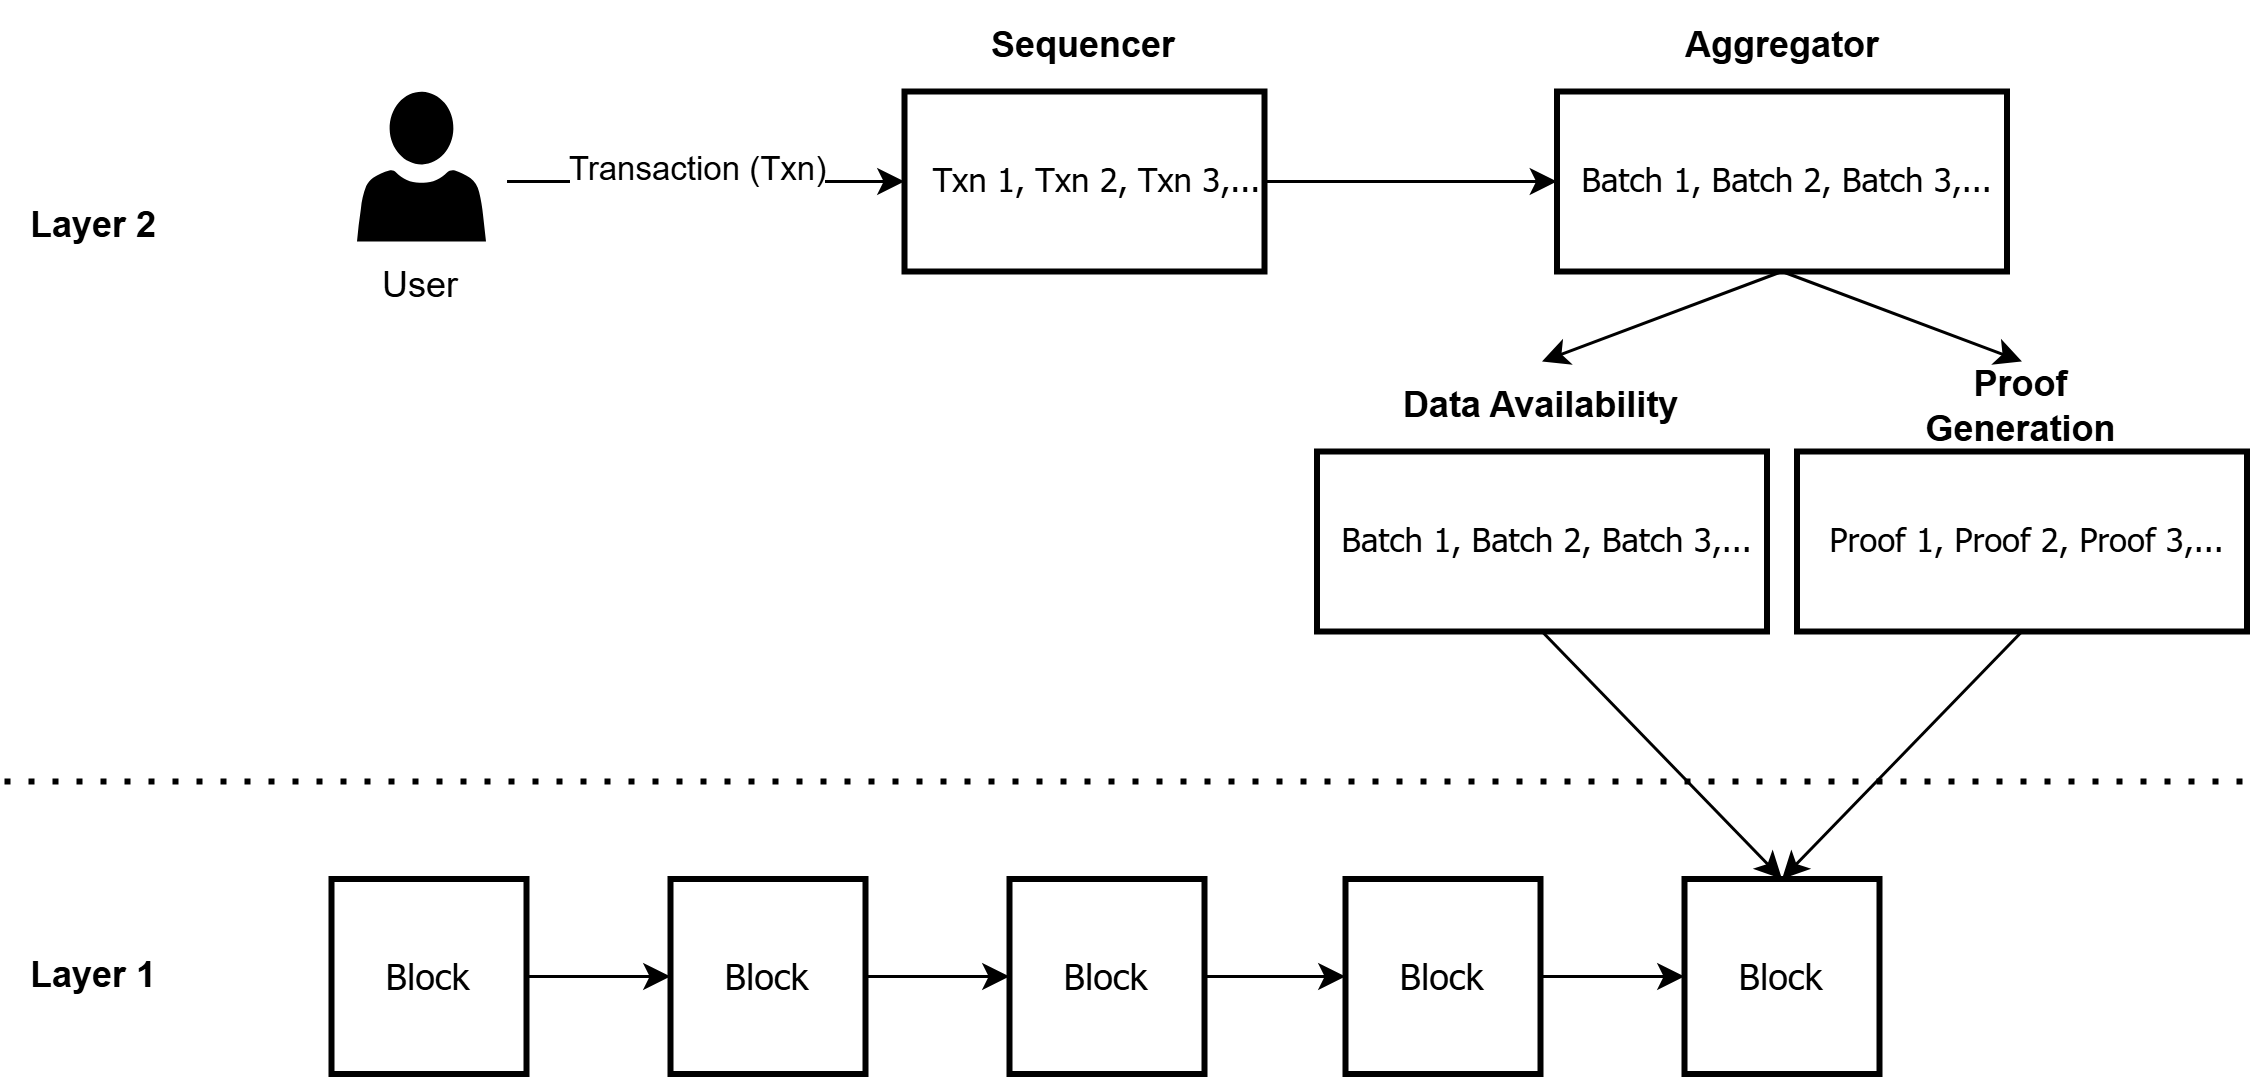
\includegraphics[width = \textwidth]{imgs/ZKRollup.png}
    \caption{Lược đồ mô tả cách ZK-Rollup hoạt động}
    \label{fig:chapter3-ZKRollup}
\end{figure}

\subsection{Cách Hoạt Động của ZK-Rollup}
Quá trình hoạt động của một hệ thống ZK-Rollup thường diễn ra như hình \ref{fig:chapter3-ZKRollup}, theo các bước sau:

\begin{enumerate}
    \item \textbf{Gửi tiền vào Rollup:} Người dùng gửi tài sản (ví dụ: token ERC-20) từ blockchain Layer 1 vào một hợp đồng thông minh trên Layer 1 được quản lý bởi ZK-Rollup. Tài sản này sau đó được ghi nhận trên ZK-Rollup ngoài chuỗi (off-chain).

    \item \textbf{Thực hiện giao dịch Off-chain:} Hàng trăm hoặc hàng nghìn giao dịch (ví dụ: chuyển token) sẽ được thực hiện ngoài chuỗi trên mạng lưới của ZK-Rollup. Các giao dịch này được tổng hợp và xử lý bởi một thực thể gọi là ``bộ tổng hợp'' (sequencer hoặc aggregator).

    \item \textbf{Tạo bằng chứng không kiến thức (ZKP):} Sau khi xử lý một lô (batch) giao dịch, bộ tổng hợp tạo ra một bằng chứng ZKP chứng minh rằng tất cả các giao dịch trong lô đó đều hợp lệ và đã được thực hiện đúng cách. Bằng chứng này rất nhỏ gọn và không tiết lộ bất kỳ thông tin chi tiết nào về các giao dịch riêng lẻ, chỉ xác nhận tính đúng đắn của chúng.

    \item \textbf{Gửi bằng chứng lên Layer 1:} Bằng chứng ZKP cùng với một bản tóm tắt nhỏ gọn về trạng thái mới của Rollup (ví dụ: gốc Merkle mới của cây trạng thái) được gửi lên hợp đồng thông minh của ZK-Rollup trên chuỗi Layer 1.

    \item \textbf{Xác minh trên Layer 1:} Hợp đồng thông minh trên Layer 1 xác minh bằng chứng ZKP. Quá trình xác minh này rất nhanh chóng và hiệu quả, bất kể số lượng giao dịch trong lô là bao nhiêu. Nếu bằng chứng hợp lệ, trạng thái mới của Rollup được cập nhật trên Layer 1, và các giao dịch trong lô được coi là đã hoàn tất.
\end{enumerate}

\subsection{Lợi Ích của ZK-Rollup}
ZK-Rollup mang lại nhiều lợi ích quan trọng cho các blockchain Layer 1:

\begin{itemize}
    \item \textbf{Khả năng mở rộng:} Bằng cách xử lý hàng nghìn giao dịch off-chain và chỉ gửi một bằng chứng duy nhất lên Layer 1, ZK-Rollup tăng đáng kể thông lượng giao dịch của blockchain nền tảng.

    \item \textbf{Giảm chi phí giao dịch:} Do ít dữ liệu được ghi lên Layer 1 hơn, phí gas cho mỗi giao dịch riêng lẻ trên ZK-Rollup được giảm thiểu đáng kể.

    \item \textbf{Bảo mật cao:} ZK-Rollup kế thừa tính bảo mật của Layer 1. Bằng chứng không kiến thức đảm bảo rằng tất cả các giao dịch off-chain đều hợp lệ về mặt mật mã, và không thể có giao dịch gian lận nào được chấp nhận trên Layer 1. Điều này khác với Optimistic Rollup, vốn dựa vào một khoảng thời gian tranh chấp.

    \item \textbf{Tính hoàn thiện tức thì (Instant Finality):} Một khi bằng chứng ZKP được xác minh trên Layer 1, các giao dịch trong lô được coi là hoàn tất ngay lập tức, không cần chờ đợi thời gian tranh chấp như các giải pháp Rollup khác.
\end{itemize}

\subsection{Token ERC-20}
ERC-20 (Ethereum Request for Comment 20) \cite{erc20} là một tiêu chuẩn kỹ thuật được sử dụng để tạo và phát hành các token có thể thay thế (fungible tokens) trên blockchain Ethereum. Tiêu chuẩn này định nghĩa một tập hợp các quy tắc chung mà tất cả các token ERC-20 phải tuân thủ, bao gồm các chức năng như chuyển token, phê duyệt chi tiêu, kiểm tra số dư, và tổng cung. Nhờ có tiêu chuẩn này, các token ERC-20 có thể tương tác dễ dàng với các ứng dụng phi tập trung (DApps), ví điện tử, sàn giao dịch và các hợp đồng thông minh khác trong hệ sinh thái Ethereum.

\subsection{Vai trò của Token ERC-20 trong ZK-Rollup}
Các giao dịch liên quan đến token ERC-20 là một trong những trường hợp sử dụng phổ biến và quan trọng nhất của ZK-Rollup. Với một số lí do sau:

\begin{itemize}
    \item \textbf{Khối lượng giao dịch lớn:} Các token ERC-20 được sử dụng rộng rãi, nên sẽ có một lượng lớn giao dịch chuyển khoản, hoán đổi, và tương tác với các hợp đồng DeFi. Việc xử lý tất cả các giao dịch này trực tiếp trên Layer 1 (Ethereum) sẽ gây ra tắc nghẽn mạng và chi phí giao dịch cao.

    \item \textbf{Tính đồng nhất:} Do các token ERC-20 tuân thủ một tiêu chuẩn chung, việc tổng hợp và xử lý chúng trong một lô giao dịch trên ZK-Rollup trở nên hiệu quả hơn. Các mạch ZKP có thể được thiết kế để xác minh tính hợp lệ của các giao dịch ERC-20 một cách đồng nhất.

    \item \textbf{Nhu cầu tối ưu hóa:} Với sự phát triển của các ứng dụng DeFi và Web3, nhu cầu về khả năng mở rộng cho các giao dịch token là rất lớn. ZK-Rollup cung cấp một giải pháp hiệu quả để đáp ứng nhu cầu này, và việc tối ưu hóa các mạch ZKP cho giao dịch ERC-20 trực tiếp góp phần vào hiệu suất tổng thể của hệ thống.
\end{itemize}

Giải pháp ZK-Rollup đóng vai trò then chốt trong việc giải quyết bài toán khả năng mở rộng của các blockchain Layer 1, đặc biệt là đối với các giao dịch token ERC-20. Bằng cách kết hợp sức mạnh của ZKP với việc xử lý off-chain, ZK-Rollup không chỉ tăng thông lượng và giảm chi phí mà còn duy trì được tính bảo mật cao. Sự phổ biến của token ERC-20 khiến việc tối ưu hóa hiệu suất xử lý các giao dịch này trên ZK-Rollup trở thành một lĩnh vực nghiên cứu và phát triển quan trọng hiện nay, trực tiếp góp phần vào sự phát triển của hệ sinh thái blockchain.

\section{zk-SNARKs và Groth16}
\subsection{zk-SNARK}
Zero-Knowledge Succinct Non-Interactive Argument of Knowledge (zk-SNARK) \cite{ballesteros2024enhancing} là một lớp các giao thức chứng minh không kiến thức cho phép một bên (người chứng minh) chứng minh cho bên kia (người xác minh) rằng họ biết một giải pháp (chứng cứ) cho một bài toán tính toán cụ thể mà không tiết lộ bất kỳ thông tin nào về giải pháp ngoài sự tồn tại của nó.

Các đặc điểm chính của zk-SNARK bao gồm tính ngắn gọn, bằng chứng được tạo ra rất nhỏ và có thể được xác minh một cách nhanh chóng, và tính không tương tác, có nghĩa là quá trình chứng minh và xác minh chỉ yêu cầu một thông điệp duy nhất từ người chứng minh đến người xác minh. Những đặc điểm này làm cho zk-SNARK đặc biệt phù hợp cho các ứng dụng blockchain, nơi mà hiệu suất xác minh và dung lượng lưu trữ là những yếu tố quan trọng.

Dưới đây là cấu trúc cơ bản của một hệ thống zk-SNARK trong thực tế, giải thích cho hình minh hoạ \ref{fig:chapter2-SNARKs_realworld}:
\begin{enumerate}
    \item \textbf{Lớp Mạch ZK:} Các lập trình viên sẽ viết mạch biểu diễn các logic sử dụng các ngôn ngữ thân thiện với SNARK như các ngôn ngữ DSL (Domain-Specific Language) như Circom, hoặc ngôn ngữ eDSL (Embedded Domain-Specific Language) như Halo2. Các mạch sẽ có hai nhiệm vụ: Đầu tiên dùng để tính toán các giá trị và tạo ra chứng cứ (witness), tiếp theo các mạch sẽ được dùng để kiểm tra tính chính xác của các chứng cứ.
    \item \textbf{Lớp Front-end:} Lớp này thường được thể hiện dưới dạng một trình biên dịch, với đầu vào là các mạch đã được viết, và đầu ra sẽ là các ràng buộc dưới dạng biểu diễn số học, ví dụ như R1CS. Front-end cũng cung cấp chức năng tạo chứng cứ (witness), sẽ nhận vào các giá trị công khai và riêng tư, kết hợp với mạch được viết và tạo ra chứng cứ (witness) tương ứng.
    \item \textbf{Lớp Back-end:} Lớp này thường được thể hiện dưới dạng một công cụ tạo bằng chứng như Snarkjs. Hỗ trợ các chức năng bao gồm: thiết lập đáng tin cậy, tạo ZKP và kiểm tra ZKP.
    \item \textbf{Lớp tích hợp (Integration Layer):} Ngoài các mạch cùng với front-end và back-end để tạo và chứng minh ZKP. Các ứng dụng thực tế thường yêu cầu thêm các phần hỗ trợ để tương tác với các thành phần SNARK ở trên. Một ví dụ với blockchain là các smart contract với chức năng xác minh nhằm xác minh các ZKP được gửi lên và thực thi logic tương ứng dựa trên kết quả xác minh.
\end{enumerate}

\subsection{Groth16}
Groth16 là một trong những giao thức zk-SNARK được sử dụng rộng rãi nhất hiện nay, được đề xuất bởi Jens Groth vào năm 2016 \cite{groth2016size}. Groth16 nổi bật nhờ một số lợi thế:
\begin{itemize}
    \item Bằng chứng cực kỳ ngắn gọn: Nó chỉ bao gồm ba phần tử trên một đường cong elliptic \cite{zhu2025extending}, bất kể kích thước của mạch.
    \item Thời gian xác minh nhanh: Quá trình xác minh chỉ yêu cầu một vài phép toán ghép cặp trên đường cong elliptic, làm cho nó phù hợp với các môi trường blockchain bị hạn chế về tài nguyên.
    \item Không tương tác: Nó chỉ yêu cầu một thông điệp từ người chứng minh đến người xác minh.
    \item Hỗ trợ cho các mạch phức tạp: Nó có thể được áp dụng cho các mạch lớn với nhiều ràng buộc, làm cho nó phù hợp với các ứng dụng như ZK-Rollup.
\end{itemize}

Tuy nhiên, Groth16 yêu cầu một giai đoạn thiết lập tin cậy cho mỗi mạch, và nếu bị xâm phạm, nó có thể ảnh hưởng đến bảo mật của hệ thống. Mặc dù vậy, các giải pháp như tính toán đa bên đã được triển khai để giảm thiểu rủi ro này trong thực tế.

Nghiên cứu này đã chọn Groth16 cho các giao dịch ERC-20 trên ZK-Rollup vì tối ưu hóa thời gian xác minh và kích thước bằng chứng là rất quan trọng để đáp ứng một số lượng lớn giao dịch cùng với yêu cầu xác minh bằng chứng liên tục. Groth16 cung cấp thời gian xác minh bằng chứng rất nhanh, bất chấp độ phức tạp của mạch hay kích thước của lô giao dịch. Thêm vào đó, nó cung cấp các bằng chứng với kích thước rất nhỏ, Groth16 là một trong những hệ thống có kích thước bằng chứng nhỏ nhất hiện có \cite{partala2020non}.

Hơn nữa, Circom cũng hỗ trợ tốt với các hệ thống chứng minh zk-SNARK như Groth16, tạo điều kiện cho việc tối ưu hóa mạch và trích xuất các tham số cần thiết để thuận tiện cho việc đánh giá.

\subsection{Luồng thực hiện tạo và xác minh bằng chứng}
Luồng tạo và xác minh bằng chứng \cite{shi2023data} \cite{ernstberger2024zk} có thể được tóm tắt như sau:
\[
\text{Circuit (R1CS)} \rightarrow \text{QAP} \rightarrow \text{Trusted Setup} \rightarrow \text{Groth16 Proving} \rightarrow \text{Verifier}
\]
%\vspace{0.5em}
\begin{enumerate}
    \item \textbf{Mạch số học (Arithmetic Circuit):} Quá trình bắt đầu bằng cách biểu diễn mạch số học của một phép toán. Mạch số học này được xây dựng bằng cách sử dụng các cổng cộng và nhân, với các dây dẫn (wires) mang giá trị thuộc một trường số nguyên tố hữu hạn \( F_p \). Mạch nhận tín hiệu đầu vào để thực hiện phép cộng và nhân theo modulo một số nguyên tố \( p \). Đầu ra của mỗi phép toán sẽ tạo ra một tín hiệu, tín hiệu này có thể là tín hiệu trung gian hoặc tín hiệu đầu ra cuối cùng của quá trình tính toán. Các ngôn ngữ lập trình mạch cấp cao như Circom thường được sử dụng để mô tả các mạch này. Một mạch sẽ được định nghĩa bởi các tín hiệu công khai, tín hiệu riêng tư, và hệ thống ràng buộc R1CS sẽ mô tả các phép toán của mạch trên các tín hiệu này.
    \item \textbf{Hệ thống ràng buộc bậc 1 (R1CS -- Rank 1 Constraint System):} Ở bước tiếp theo, ta chuyển đổi mạch số học thành hệ thống R1CS. R1CS là một đại diện trung gian phổ biến cho các mạch ZKP, được sử dụng bởi các công cụ frontend như Circom và ZoKrates\cite{eberhardt2018zokrates}. Biểu diễn R1CS bao gồm một tập hợp các ràng buộc, mỗi ràng buộc có một ràng buộc bậc nhất tương ứng với một cổng nhân trong mạch, được biểu diễn dưới dạng \( a \times b = c \). Tập hợp của tất cả các ràng buộc như vậy sẽ tạo thành một hệ thống các ràng buộc cấp độ 1.
    \item \textbf{Chương trình số học bậc 2 (QAP -- Quadratic Arithmetic Program):} Để phù hợp với các kỹ thuật mã hóa zk-SNARK, hệ thống R1CS được chuyển đổi tiếp trở thành một ``Chương trình số học bậc hai'' (QAP -- Quadratic Arithmetic Program). QAP mã hóa các ràng buộc của R1CS vào các đa thức đại số, ở đây các giá trị chứng cứ (witness) sẽ được đưa vào các hệ số của những đa thức này. Nếu một chứng cứ hợp lệ tồn tại, đa thức \( Q(x) \) (được xây dựng từ chứng cứ và các ràng buộc) sẽ chia hết cho một đa thức mục tiêu \( Z(x) \) (được định nghĩa bởi cấu trúc mạch). Do đó, người chứng minh cần phải chứng minh sự tồn tại của một đa thức \( H(x) \) sao cho \( Q(x) = H(x) \times Z(x) \), mà không tiết lộ trực tiếp chứng cứ hoặc các đa thức này. Việc chuyển đổi sang QAP là một bước quan trọng để áp dụng các giao thức chứng minh không kiến thức hiệu quả và an toàn.
    \item \textbf{Thiết Lập Tin Cậy (Trusted Setup):} Giai đoạn thiết lập tin cậy là một bước quan trọng để tạo ra các khóa mật mã cần thiết cho việc tạo và xác minh bằng chứng. Đối với Groth16, quy trình này thường bao gồm hai giai đoạn. Giai đoạn 1 (Powers of Tau -- một giao thức tính toán đa bên) tạo ra các giá trị bí mật ngẫu nhiên chung cho toàn bộ hệ thống. Giai đoạn 2 (thiết lập cụ thể cho từng mạch) sử dụng kết quả từ giai đoạn 1 và cấu trúc cụ thể của mạch (thông qua QAP) để tạo ra khóa chứng minh và khóa xác minh. Việc đảm bảo tính bí mật của các giá trị ngẫu nhiên được tạo ra trong quá trình này là rất quan trọng để duy trì bảo mật của hệ thống.
    \item \textbf{Tạo bằng chứng (Proving):} Trong quá trình tạo bằng chứng, người chứng minh sử dụng khóa chứng minh (được tạo ra trong giai đoạn thiết lập tin cậy) và chứng cứ (các giá trị bí mật thỏa mãn mạch) để tạo ra một bằng chứng \( \pi \). Các giá trị đầu vào công khai cũng được cung cấp cho người xác minh sử dụng trong quá trình xác minh. Bằng chứng \( \pi \) thường có kích thước rất nhỏ.

    \item \textbf{Xác minh bằng chứng (Verifying Proof):} Cuối cùng, người xác minh sử dụng khóa xác minh (cũng được tạo ra trong giai đoạn thiết lập tin cậy), bằng chứng \( \pi \) nhận được từ người chứng minh, và các giá trị đầu vào công khai để kiểm tra tính hợp lệ của bằng chứng chứng. Quá trình xác minh thường sử dụng một số phép toán ghép cặp trên đường cong elliptic, kết quả sẽ là chấp nhận hoặc từ chối bằng chứng.
\end{enumerate}

\section{Trình biên dịch Circom và các mức tối ưu hoá ràng buộc}
\subsection{Trình biên dịch Circom}
Circom \cite{belles2022circom} \cite{munoz2023circom} là một ngôn ngữ mô tả mạch (Circuit Description Language) và là một trình biên dịch (compiler) được thiết kế đặc biệt để xây dựng các mạch số học cho các bằng chứng không kiến thức (ZKP), đặc biệt là zk-SNARKs. Circom được phát triển để đơn giản hóa quá trình thiết kế và triển khai các mạch ZKP phức tạp, vốn thường đòi hỏi kiến thức sâu về mật mã và toán học. Nó cho phép các nhà phát triển định nghĩa các tính toán dưới dạng mạch số học một cách trực quan hơn, sau đó biên dịch chúng thành định dạng R1CS (Rank-1 Constraint System) mà các hệ thống zk-SNARK có thể sử dụng.

Các đặc điểm nổi bật của Circom:
\begin{itemize}
    \item \textbf{Kiểu lập trình tương tự các ngôn ngữ lập trình phần cứng:} Kiểu lập trình mô tả trực tiếp từng ràng buộc của Circom giúp lập trình viên kiểm soát tối đa từng constraint được sinh ra, giúp tạo các bằng chứng ZK nhỏ gọn, nhanh và tiết kiệm chi phí nhất.
    \item \textbf{Tính mô-đun:} Circom hỗ trợ khái niệm "template" (mẫu), cho phép tạo ra các mạch con có thể tái sử dụng và tham số hóa. Điều này giúp xây dựng các mạch lớn hơn từ các thành phần cơ bản, tăng cường khả năng tái sử dụng mã và giảm độ phức tạp khi triển khai mạch.
    \item \textbf{Hỗ trợ biên dịch R1CS}: Chức năng chính của trình biên dịch Circom là chuyển đổi mã Circom thành một tập hợp các ràng buộc R1CS, cùng với các tệp hỗ trợ khác (như tệp wasm hoặc c++ để tính toán chứng cứ).
    \item \textbf{Hệ sinh thái:} Circom là một phần của một hệ sinh thái lớn hơn bao gồm circomlib (thư viện các template mạch phổ biến) và snarkjs (thư viện JavaScript để tạo và xác minh bằng chứng zk-SNARK) cùng các công cụ hỗ trợ khác như circomspect, circomkit,... Giúp các nhà phát triển thuận tiện hơn trong việc xây dựng các ứng dụng ZK.
    \item \textbf{Là trình biên dịch và ngôn ngữ đã phát triển và được sử dụng rộng rãi:} Circom phát triển được qua hai phiên bản ổn định với nhiều cải tiến giúp thuận tiện hơn cho người sử dụng, đồng thời đã được ứng dụng trong nhiều dự án thực tế như ứng dụng gửi tiền ẩn danh trên Ethereum Tornado Cash \cite{khovratovich2019tornado} và ZK-Rollup Hermez Network, là tiền thân của ZK-Rollup Polygon Hermez hiện nay.
\end{itemize}

\subsection{Cơ chế tối ưu hoá ràng buộc trong Circom}
\label{Cơ chế tối ưu hoá ràng buộc trong Circom}
Trong các hệ thống zk-SNARK, số lượng ràng buộc trong mạch R1CS có ảnh hưởng trực tiếp đến hiệu suất của quá trình tạo bằng chứng (proving time) và kích thước của bằng chứng (proof size). Càng ít ràng buộc, quá trình tạo bằng chứng càng nhanh và bằng chứng càng nhỏ. Circom cung cấp các cờ tối ưu hóa khác nhau để giúp giảm số lượng ràng buộc được tạo ra trong quá trình biên dịch.

Các cờ tối ưu hóa này hoạt động bằng cách áp dụng các kỹ thuật biến đổi đại số để loại bỏ các ràng buộc dư thừa hoặc đơn giản hóa các ràng buộc hiện có. Dưới đây là các mức tối ưu hóa chính được hỗ trợ bởi trình biên dịch Circom:

\begin{enumerate}
    \item \textbf{--O0 (Không tối ưu hóa):}
    \begin{itemize}
        \item Đây là mức tối ưu hóa thấp nhất, nơi trình biên dịch không áp dụng bất kỳ kỹ thuật tối ưu hóa ràng buộc nào. Mỗi phép toán trong mạch Circom sẽ được chuyển đổi trực tiếp thành các ràng buộc R1CS tương ứng mà không có sự đơn giản hóa nào.
    \end{itemize}
    \item \textbf{--O1 (Tối ưu hóa cơ bản - Mặc định):}
    \begin{itemize}
        \item Đây là mức tối ưu hóa mặc định của trình biên dịch Circom. Nó áp dụng các tối ưu hóa cơ bản nhưng hiệu quả để giảm số lượng ràng buộc.
        \item Các tối ưu hóa chính ở mức --O1 bao gồm việc loại bỏ các ràng buộc có dạng \texttt{signal = k} (trong đó \texttt{k} là một hằng số) và \texttt{signal1 = signal2}. Trình biên dịch sẽ thay thế tất cả các lần xuất hiện của \texttt{signal} bằng \texttt{k} hoặc thay \texttt{signal1} bằng \texttt{signal2} (hoặc ngược lại, tùy thuộc vào việc một trong các tín hiệu là riêng tư để duy trì tính đúng đắn của bằng chứng).
    \end{itemize}
    \item \textbf{--O2 (Tối ưu hóa nâng cao):}
    \begin{itemize}
        \item Mức --O2 bao gồm tất cả các tối ưu hóa của --O1 và áp dụng thêm các kỹ thuật tối ưu hóa nâng cao hơn, đặc biệt là sử dụng khử Gauss dạng "lười" (Lazy Form of Gaussian Elimination).
        % \item Mục tiêu của -O2 là loại bỏ càng nhiều ràng buộc tuyến tính càng tốt, đặc biệt là những ràng buộc chứa ít nhất một tín hiệu riêng tư. Sau khi áp dụng các phép thế được phát hiện bởi thuật toán, một số ràng buộc phi tuyến tính có thể trở thành tuyến tính, và quá trình khử Gauss sẽ được thực hiện lặp đi lặp lại cho đến khi không còn ràng buộc tuyến tính nào chứa tín hiệu riêng tư có thể được loại bỏ.
        % \item Trong Groth16, chi phí của phép cộng được coi là miễn phí, nghĩa là không cần tạo thêm ràng buộc khi phép cộng xuất hiện trong biểu thức. Tối ưu hóa -O2 tận dụng triệt để đặc điểm này để đơn giản hóa mạch mà không ảnh hưởng đến tính đúng đắn của bằng chứng.
        \item Nguyên lý cốt lõi của tối ưu hóa -O2 dựa trên nhận định rằng các cổng cộng (addition gates) trong mạch số học được coi là ``miễn phí'' trong các hệ thống zk-SNARK như Groth16 \cite{albert2022distilling} \cite{diaz2023extending}. Điều này có nghĩa là việc thêm các phép cộng không làm tăng số lượng ràng buộc. Tận dụng điều này, -O2 tìm cách loại bỏ các ràng buộc tuyến tính (linear constraints) bằng cách thay thế một tín hiệu (signal) trong ràng buộc đó bằng một biểu thức tuyến tính tương đương. Quá trình này được thực hiện lặp đi lặp lại cho đến khi không còn ràng buộc tuyến tính nào chứa ít nhất một tín hiệu riêng tư có thể được đơn giản hóa thêm.
        \item Cụ thể, thuật toán khử Gauss dạng lười hoạt động theo nhiều vòng lặp (rounds). Trong mỗi vòng, nó xác định các ràng buộc tuyến tính và cố gắng loại bỏ các tín hiệu bằng cách tạo ra các phép thế (substitutions). Điều đặc biệt của tính "lười" là sau một số lượng vòng lặp, khi một số phép thế được áp dụng, một số ràng buộc phi tuyến tính ban đầu có thể trở thành tuyến tính. Khi đó, thuật toán sẽ tiếp tục các vòng lặp khử Gauss cho đến khi không còn ràng buộc tuyến tính mới nào được tìm thấy hoặc đạt đến điều kiện dừng. Hình \ref{fig:chapter3-SimplficationExample} minh hoạ một trường hợp đơn giản của quá trình tối ưu ràng buộc trong mạch, trong đó "signal C" là một tín hiệu riêng tư (private signal); trong trường hợp này, trình biên dịch có thể nội suy biểu thức để giảm số lượng ràng buộc.

    \end{itemize}
\end{enumerate}

\begin{figure}[H]
    \centering
    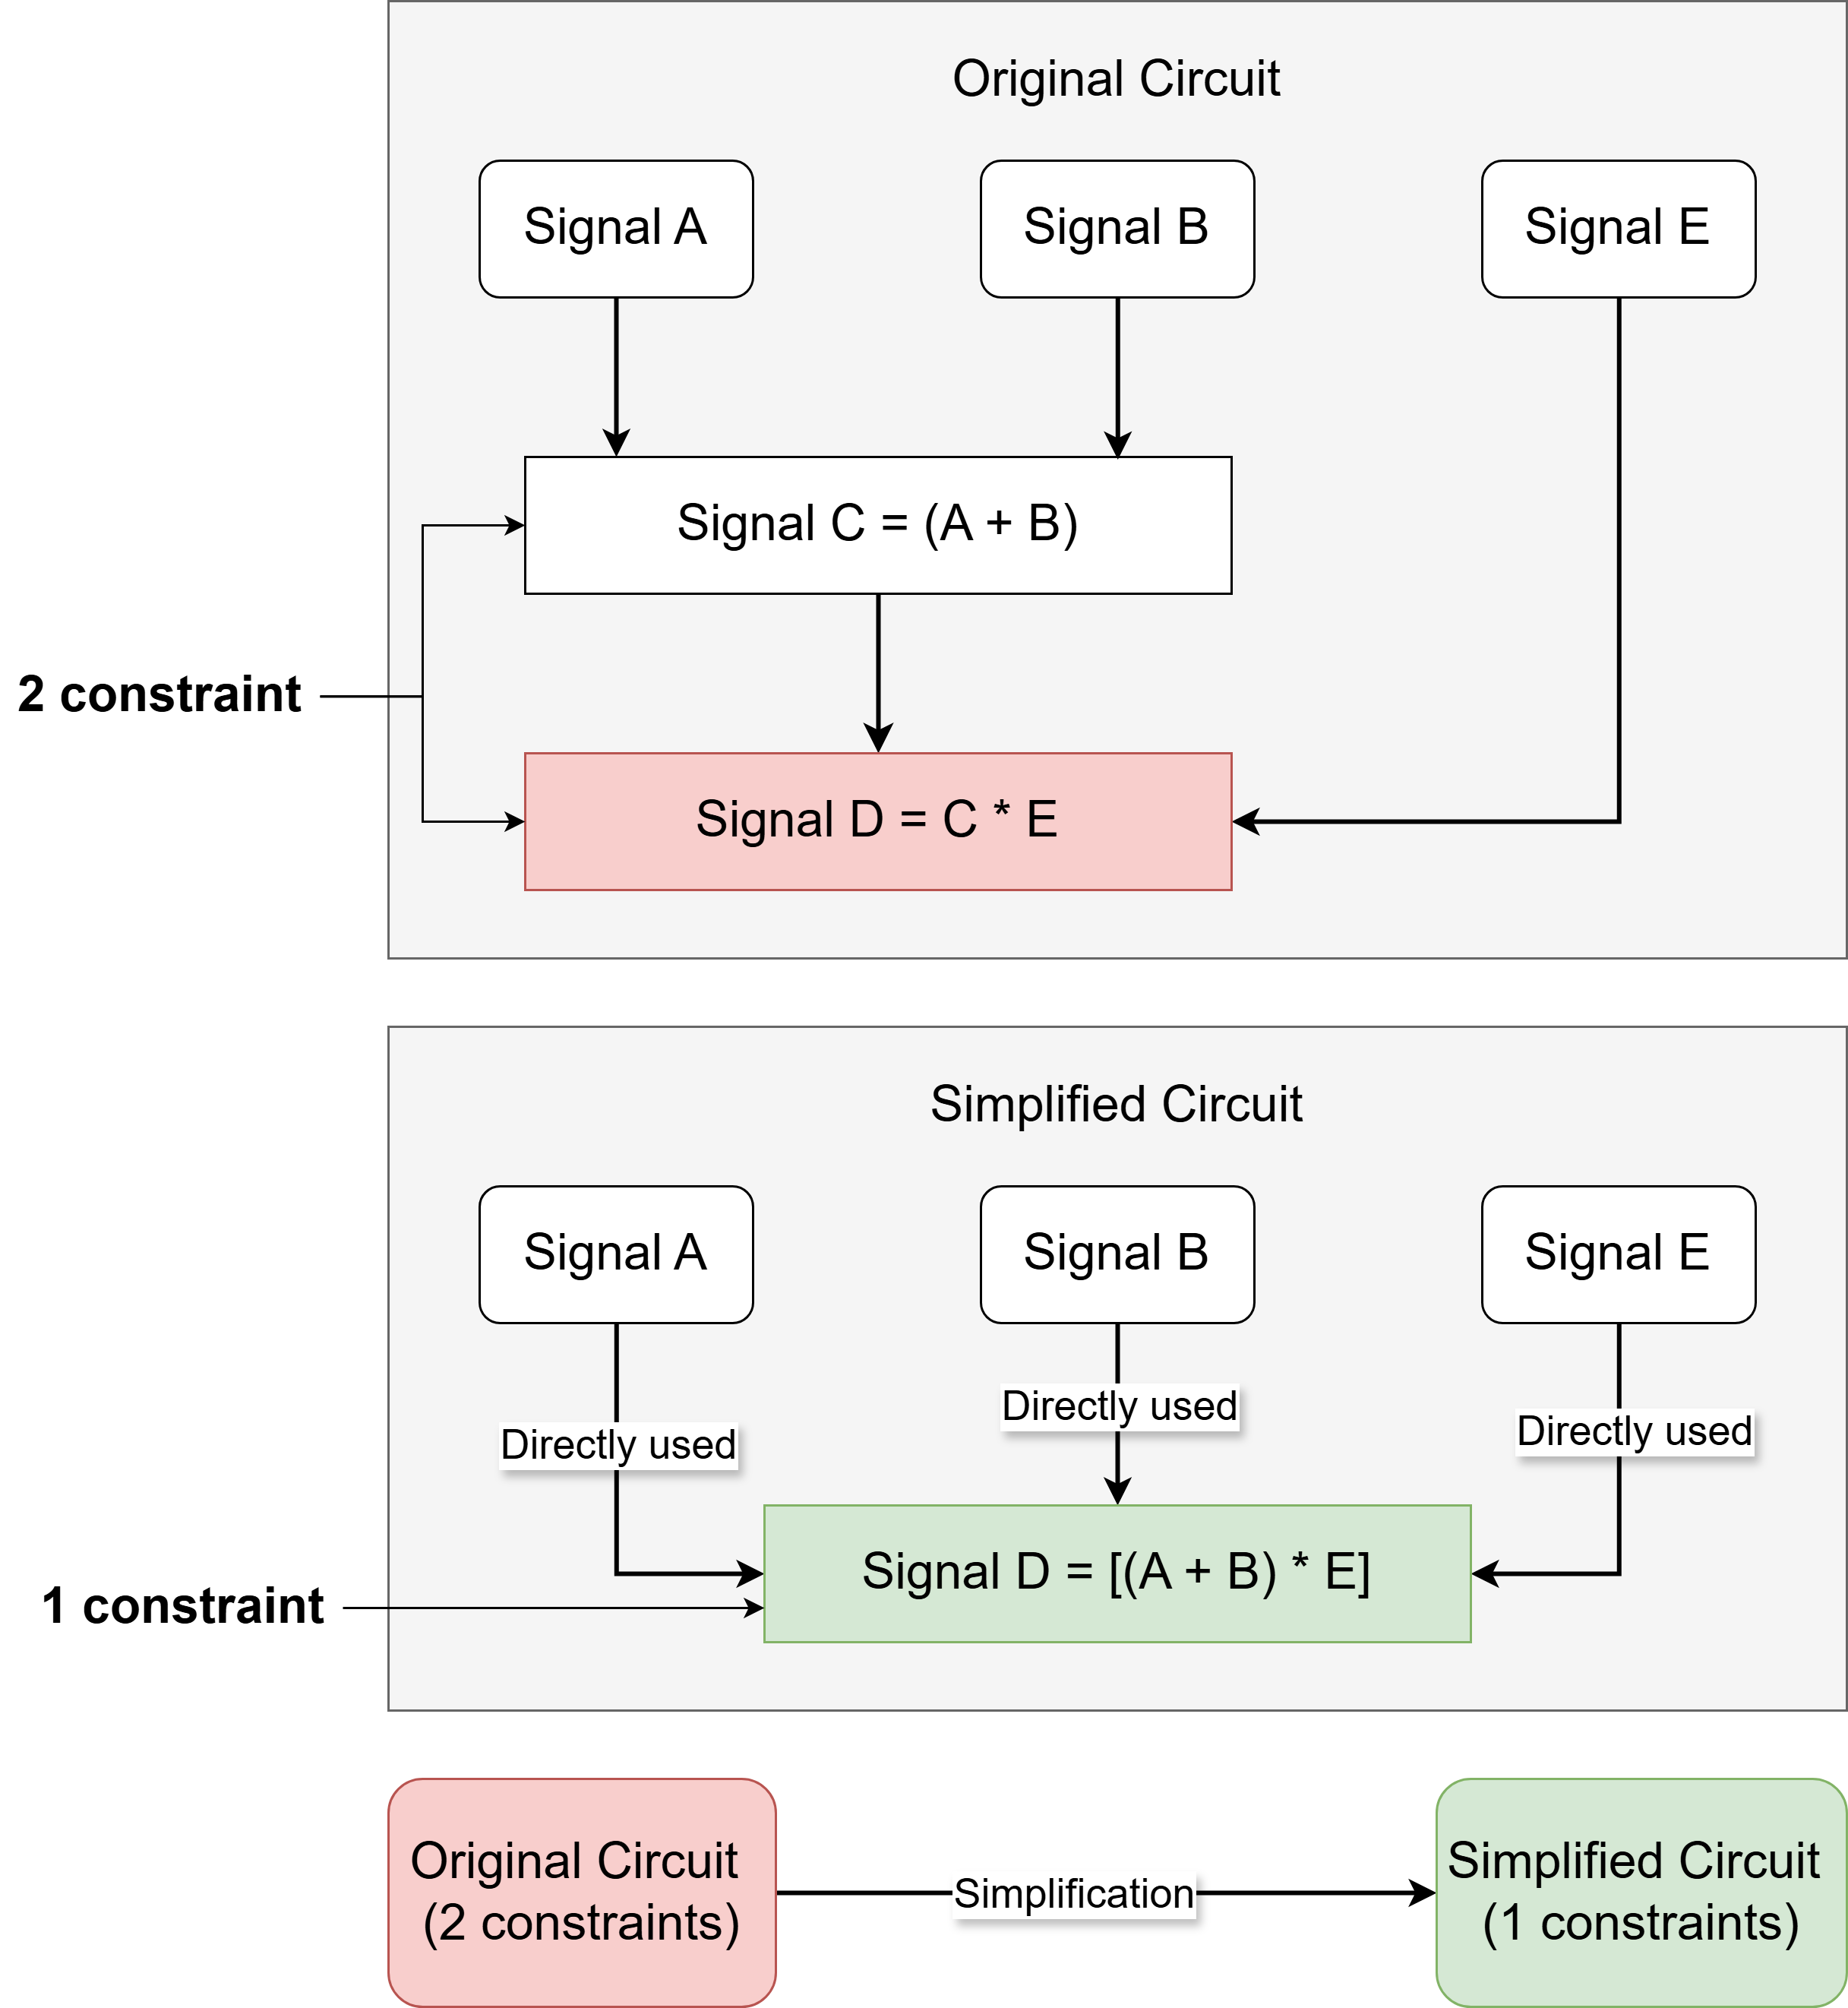
\includegraphics[width = 0.7\textwidth]{imgs/SimplificationExample.png}
    \caption{Lược đồ minh hoạ quá trình tối ưu ràng buộc}
    \label{fig:chapter3-SimplficationExample}
\end{figure}

\section{Phân tích mức tối ưu hóa --O2}

Qua thực nghiệm, nghiên cứu nhận thấy rằng việc sử dụng cờ tối ưu hóa --O2 của trình biên dịch Circom dẫn đến sự gia tăng đáng kể về thời gian biên dịch mạch so với các cờ --O0 và --O1. Đặc biệt hơn, nghiên cứu nhận thấy thời gian thực hiện các vòng lặp khử Gauss không phải là giai đoạn tốn nhiều thời gian nhất trong quá trình tối ưu --O2, mà chính bước khử Gauss đầu tiên trước khi áp dụng các vòng lặp khử Gauss gây tốn nhiều thời gian hơn cả. Để tìm hiểu nguyên nhân, em đã tiến hành phân tích hoạt động của mã nguồn trình biên dịch Circom và nhận thấy rằng sự khác biệt chủ yếu đến từ khối lượng lớn ràng buộc tuyến tính mà bước khử Gauss trong --O2 cần phải xử lí. Dưới đây là phân tích chi tiết:

\subsection{Sự khác biệt cốt lõi trong quy trình tối ưu hóa}

Điểm khác biệt chính giữa --O1 và --O2 nằm ở việc --O2 sử dụng một quy trình tối ưu hóa tuyến tính bổ sung mà --O1 không được áp dụng. 

Với --O1, trình biên dịch chỉ thực hiện các bước đơn giản hóa cơ bản và không áp dụng các thuật toán phức tạp để giảm ràng buộc tuyến tính. Các ràng buộc tuyến tính chỉ được loại bỏ thông qua các phép thay thế đơn giản như đề cập ở \ref{Cơ chế tối ưu hoá ràng buộc trong Circom}. 

Với --O2, trình biên dịch sử dụng một cơ chế đơn giản hóa tuyến tính dựa trên cụm (cluster-based linear simplification). Đây là một hoạt động đòi hỏi nhiều tính toán cùng với lượng lớn ràng buộc tuyến tính cần xử lí là nguyên nhân chính gây ra sự khác biệt về thời gian biên dịch.

\subsection{Các giai đoạn xử lý chung và chi phí}

% Cả --O1 và --O2 đều thực hiện các bước xử lý cơ bản, nhưng chi phí của chúng tăng lên đáng kể khi mạch trở nên phức tạp hơn, đặc biệt là khi các kết quả của các bước xử lý này được sử dụng làm đầu vào cho các bước tối ưu hóa sâu hơn của --O2:

% \begin{itemize}
%     \item \textbf{Xây dựng tập hợp tín hiệu liên quan:} Trình biên dịch cần xác định tất cả các tín hiệu thuộc các ràng buộc phi tuyến và các mối quan hệ phụ thuộc giữa chúng với nhau. Quá trình này bao gồm việc duyệt qua toàn bộ biểu diễn đồ thị của mạch và xác định các tín hiệu cần phải giữ lại.
%     \item \textbf{Khử các ràng buộc đẳng thức đơn giản:} Các ràng buộc đơn giản như \texttt{signal = k} (trong đó \texttt{k} là một hằng số) và \texttt{signal1 = signal2} được xử lý.
%     \item \textbf{Xây dựng lại tập hợp các tín hiệu liên quan:} Tính toán lại các tín hiệu liên quan sau khi áp dụng các phép thế của bước ``Đơn giản hóa các ràng buộc đẳng thức''.
    
% \end{itemize}

Cả hai mức tối ưu –O1 và –O2 đều thực hiện các bước xử lý cơ bản trong quá trình biên dịch, tuy nhiên chi phí xử lý có xu hướng gia tăng đáng kể khi độ phức tạp của mạch tăng lên. Điều này đặc biệt rõ ràng khi các kết quả từ các bước xử lý cơ bản được sử dụng làm đầu vào cho các giai đoạn tối ưu hóa sâu hơn trong –O2.

Bước đầu tiên trình biên dịch thực hiện là xây dựng tập hợp các tín hiệu liên quan. Trình biên dịch cần xác định tất cả các tín hiệu tham gia vào các ràng buộc phi tuyến cũng như các mối quan hệ phụ thuộc giữa chúng. Quá trình này đòi hỏi việc duyệt qua toàn bộ biểu diễn đồ thị của mạch để xác định các tín hiệu cần được giữ lại nhằm đảm bảo tính toàn vẹn trong quá trình đơn giản hóa.

Tiếp theo, trình biên dịch tiến hành khử các ràng buộc đẳng thức đơn giản. Những ràng buộc có dạng như signal = k (với k là một hằng số) hoặc signal1 = signal2 sẽ được xử lý thông qua các phép thay thế trực tiếp, nhằm giảm số lượng ràng buộc một cách hiệu quả mà không ảnh hưởng đến tính đúng đắn của mạch.

Sau khi thực hiện các phép thay thế, trình biên dịch cần xây dựng lại tập hợp các tín hiệu liên quan. Việc này bao gồm việc tính toán lại toàn bộ các tín hiệu còn hoạt động sau khi biểu đồ ràng buộc đã được cập nhật. Quá trình này đảm bảo rằng các bước tối ưu hóa tiếp theo có thể hoạt động trên một tập hợp tín hiệu chính xác và tối thiểu, từ đó nâng cao hiệu quả tối ưu hóa tổng thể.

\subsection{Các hoạt động tối ưu hóa nâng cao của --O2}

Thời gian biên dịch tăng lên đáng kể ở --O2 chủ yếu do các hoạt động tính toán sau đây, được kích hoạt bởi cơ chế tối ưu hóa tuyến tính của --O2:

\begin{itemize}
    \item \textbf{Đơn giản hóa tuyến tính dựa trên cụm:} Đây là hoạt động tối ưu hóa quan trọng nhất của --O2. Trình biên dịch thực hiện khử Gauss với xử lý song song, nhóm các ràng buộc liên quan thành các cụm có chung tín hiệu. Mặc dù việc xử lý song song giúp tăng tốc độ trong các vòng lặp chính, nhưng với khối lượng ràng buộc rất lớn của mạch ZK-Rollup, thời gian xử lí của quá trình này vẫn tăng lên đáng kể.
    \item \textbf{Nhiều vòng lặp tối ưu hóa:} --O2 không chỉ thực hiện tối ưu hóa một lần mà lặp đi lặp lại nhiều vòng cho đến khi không còn ràng buộc tuyến tính nào có thể được đơn giản hóa thêm. Mỗi vòng lặp đòi hỏi việc kiểm tra, xử lý lại các ràng buộc, và đặc biệt là việc xác định khi nào các ràng buộc phi tuyến tính ban đầu trở thành tuyến tính sau các phép thế. Quá trình lặp này làm tăng đáng kể tổng thời gian xử lý.
    \item \textbf{Quản lý cấu trúc dữ liệu:} Để thực hiện các tối ưu hóa sâu, trình biên dịch cần xây dựng và duy trì nhiều cấu trúc dữ liệu trong bộ nhớ để theo dõi các tín hiệu như ràng buộc và các phép thế. Việc quản lý và truy cập liên tục vào các cấu trúc này, đặc biệt với các mạch lớn, tiêu tốn nhiều tài nguyên bộ nhớ và thời gian xử lý.
    \item \textbf{Thay thế và xử lý lại ràng buộc:} Trong mỗi vòng lặp tối ưu hóa, các phép thế được áp dụng cho tất cả các ràng buộc. Sau đó, hệ thống phải kiểm tra lại toàn bộ tập hợp ràng buộc để xác định những ràng buộc nào đã trở thành tuyến tính và cần được xử lý tiếp. Quá trình duyệt và cập nhật liên tục này là một yếu tố chính gây tốn thời gian.
    \item \textbf{Cơ chế kiểm soát vòng lặp:} Mặc dù trình biên dịch có tham số để giới hạn số vòng lặp tối đa, nhưng chính vòng lặp đầu tiên đã chịu phần xử lí nhiều nhất cho lượng lớn ràng buộc tuyến tính làm đầu vào ban đầu.
\end{itemize}

\subsection{Kết luận}

Tóm lại, sự gia tăng đáng kể về thời gian biên dịch của cờ --O2 so với --O0 và --O1 không phải hoàn toàn do các vòng lặp khử Gauss xử lí chậm, mà còn do chi phí thiết lập ban đầu cao trước khi bắt đầu thực hiện các vòng lặp. Các giai đoạn xử lý này bao gồm việc xây dựng các cấu trúc dữ liệu, thực hiện nhiều lần duyệt qua các ràng buộc, và các thao tác bộ nhớ khác trên lượng ràng buộc tuyến tính lớn ở đầu vào. Mặc dù tốn kém về thời gian biên dịch, những chi phí này là cần thiết để đạt được mức độ giảm ràng buộc tối đa, từ đó dẫn đến thời gian tạo bằng chứng nhanh hơn và kích thước bằng chứng nhỏ hơn, điều này đặc biệt quan trọng trong môi trường sản xuất nơi việc tạo bằng chứng được thực hiện thường xuyên.
\chapter{ZCLS: Chiến lược tối ưu ràng buộc theo vòng đời phát triển mạch ZKP}
\label{chap:chap4}
\section{Phương pháp thực nghiệm}
\subsection{Mô tả thực nghiệm}
Nghiên cứu này được thiết kế dưới dạng một thực nghiệm định lượng nhằm đánh giá tác động của các cờ tối ưu hóa ràng buộc trong trình biên dịch Circom lên hiệu suất của một hệ thống ZK-Rollup mô phỏng cho các giao dịch ERC-20. Từ đó 
xây dựng khung gợi ý sử dụng cờ tối ưu ràng buộc mạch \textbf{ZCLS}.

Việc triển khai hệ thống ZK-Rollup mô phỏng được trình bày ở phần này, cùng với ứng dụng CirMetrics được mô tả trong các phần tiếp theo, được lưu trữ ở nguồn GitHub ZCLS-for-CirMetrics\footnote{\url{https://github.com/datachain-uit/ZCLS-for-CirMetrics}}.

Các tham số chính trong nghiên cứu này là các cờ tối ưu hóa ràng buộc của Circom (--O0, --O1, --O2) và kích thước lô giao dịch (8, 16, 32 và 64 giao dịch).
Hệ thống ZK-Rollup được triển khai bao gồm các chức năng chính như: gửi tiền vào layer 2 (ZK-Rollup), chuyển khoản và rút tiền về layer 1.

Để đánh giá hiệu suất, hai mạch chứng minh không kiến thức chính đã được thiết kế gồm:

\begin{itemize}
    \item \textbf{Mạch xử lý giao dịch theo lô:} Mạch này được sử dụng để tạo ra các chứng minh cho các lô giao dịch được xử lý ngoài chuỗi, cho phép blockchain layer 1 xác minh tính chính xác của các giao dịch này. Số lượng ràng buộc trong mạch này thay đổi đáng kể theo số lượng giao dịch được xử lý trong lô.
    \item \textbf{Mạch xử lý rút tiền:} Mạch này hỗ trợ rút tiền từ lớp 2 sang lớp 1 và có số lượng ràng buộc ổn định hơn, với những biến đổi nhẹ tùy thuộc vào số lượng tối đa giao dịch được xử lý trong lô.
\end{itemize}

Trong thí nghiệm này, nghiên cứu chủ yếu tập trung vào việc đánh giá hiệu suất của mạch xử lý giao dịch theo lô, vì nó đại diện cho một mạch phức tạp bao trùm chức năng chính của ZK-Rollup và phản ánh rõ ràng các yêu cầu về hiệu suất và tính toán liên quan đến việc xử lý nhiều giao dịch đồng thời.

Các kích thước lô giao dịch (8, 16, 32 và 64 giao dịch) được lựa chọn để đại diện cho các kịch bản giao dịch phổ biến trong ZK-Rollup, từ các lô nhỏ đến các lô có kích thước trung bình, cho phép quan sát xu hướng hiệu suất khi số lượng giao dịch tăng lên. Đây là các kích thước lô phù hợp để sử dụng trong các nghiên cứu và triển khai ZK-Rollup để đánh giá hiệu suất ban đầu.

\subsection{Cấu Hình Phần Cứng và Phần Mềm}
Cấu hình thí nghiệm được giới hạn với cấu hình thiết bị cố định bao gồm: phần cứng sử dụng bộ xử lý AMD Ryzen thế hệ 8 với 8 lõi và 16 luồng, cùng với 32 GB RAM. Cấu hình này mô phỏng phần cứng của một máy tính tầm trung dành cho cá nhân với đa mục đích sử dụng.


\subsection{Độ đo sử dụng}
Để đánh giá hiệu suất của các cấu hình ZK-Rollup khác nhau, nghiên cứu đã sử dụng một số độ đo tham khảo ở các công trình nghiên cứu về ZK-Rollup \cite{chaliasos2024analyzing} cũng như hệ thống ràng buộc R1CS \cite{albert2022distilling} và các hệ thống ZKP \cite{el2024evaluating} như sau:
\begin{itemize}
    \item Tổng số lượng ràng buộc:
    \begin{itemize}
        \item Tổng số lượng ràng buộc (bao gồm cả ràng buộc tuyến tính và phi tuyến).
        \item Số lượng ràng buộc tuyến tính và phi tuyến riêng biệt.
    \end{itemize}
    Số lượng ràng buộc sẽ ảnh hưởng trực tiếp đến chi phí và thời gian tạo ZKP. Độ đo này sẽ giúp nghiên cứu đánh giá độ phức tạp và hiệu quả của mạch ZK.
    \item Thời gian biên dịch (Compilation time): Thời gian cần thiết để trình biên dịch Circom chuyển đổi mã mạch thành R1CS và các tệp liên quan. Đây là thông số quan trong khi các nhà phát triển đang xây dựng mạch ZK, ảnh hưởng trực tiếp đến thời gian phát triển và triển khai ứng dụng.
    \item Thời gian tạo bằng chứng (Proving time): Thời gian cần thiết cho thư viện Snarkjs để tạo ra ZKP cho một lô giao dịch. Độ đo này phản ánh hiệu quả của hệ thống ZK-Rollup, thời gian tạo bằng chứng càng nhanh, giao dịch sẽ được xác minh càng sớm, giúp gia tăng thông lượng cho hệ thông ZK-Rollup.
    \item Thời gian xác minh bằng chứng (Verifying time): Thời gian cần thiết để xác minh tính hợp lệ của chứng minh, được đo cả ở ngoài chuỗi và trên chuỗi. Đây là độ đo phản ánh thời gian cần thiết để giao dịch được xác minh sau khi bằng chứng được gửi lên Layer 1, ảnh hưởng trực tiếp đến trải nghiệm người dùng và tốc độ kết thúc giao dịch.
    \item Tiêu thụ gas: Số lượng gas tiêu thụ trên blockchain lớp 1 cho việc xác minh chứng minh, độ đo này ảnh hưởng đến chi phí, ví dụ như số lượng Ethereum hoặc native coin (đồng tiền gốc) của ZK-Rollup người dùng cần trả khi thực hiện giao dịch.
\end{itemize}

Dữ liệu cho các chỉ số này đã được thu thập cho từng cờ tối ưu hóa và kích thước lô giao dịch được thử nghiệm.

\subsection{Số lần chạy thử nghiệm và sai số}
Để đảm bảo tính tin cậy và chính xác của các kết quả thực nghiệm, mỗi phép đo về thời gian biên dịch mạch và thời gian tạo bằng chứng đều được thực hiện lặp lại nhiều lần.

Vì thí nghiệm được thực nghiệm với chỉ một cấu hình thiết bị cụ thể, tập trung vào việc phân tích so sánh hiệu quả giữa các mức tối ưu hoá, nghiên cứu thực hiện chạy mỗi cấu hình thí nghiệm lặp lại 10 lần. Sau đó, giá trị trung bình của các lần đo được sử dụng làm kết quả chính thức cho cấu hình đó. Cách tiếp cận này phù hợp tương tự trường hợp thực tiễn đã được thiết lập trong nghiên cứu đánh giá hiệu năng ZKP \cite{ernstberger2024zk}, khi các điều kiện được kiểm soát sẽ cho phép thu thập số liệu đáng tin cậy với số lần đo nhỏ.

Việc lặp lại phép đo giúp giảm thiểu ảnh hưởng của các yếu tố ngẫu nhiên và nhiễu hệ thống như mức độ tải của hệ thống hoặc các tiến trình nền, các yếu tố này có thể làm sai lệch kết quả đo thời gian.
Công thức tính giá trị trung bình được biểu diễn như sau:
\[
\bar{x} = \frac{1}{N} \sum_{i=1}^{N} x_i
\]


\subsection{Kế Hoạch Phân Tích}
Dữ liệu thu thập sẽ được phân tích định lượng để đạt được các mục tiêu nghiên cứu. Kế hoạch phân tích được trình bày như sau:
\begin{itemize}
    \item Phân tích mối quan hệ giữa ràng buộc và hiệu suất: Phân tích mối quan hệ giữa số lượng ràng buộc và thời gian biên dịch lẫn thời gian sinh chứng minh.
    \item Đánh giá các yếu tố đánh đổi: Định lượng các yếu tố đánh đổi giữa thời gian biên dịch (chi phí phát triển ứng dụng) và thời gian tạo bằng chứng (hiệu quả hoạt động của ứng dụng) cho mỗi cờ tối ưu hóa. Các biểu đồ hình ảnh sẽ được sử dụng để minh họa các yếu tố đánh đổi này.
    \item Phát triển một khung tối ưu hóa: Dựa trên các kết quả thí nghiệm, nghiên cứu sẽ đề xuất một khung tối ưu hóa đa mạch, phù hợp với các giai đoạn phát triển. Khung này sẽ cung cấp hướng dẫn thực tiễn cho các nhà phát triển ZK-Rollup trong việc chọn lựa các cờ tối ưu hóa Circom dựa trên các ưu tiên cụ thể của dự án (ví dụ tốc độ lặp lại trong phát triển so với yêu cầu về thông lượng trong sản phẩm thực tế) và đặc điểm của mỗi mạch.
\end{itemize}

\section{Kiến trúc hệ thống}
\subsection{Các thư viện và công cụ được sử dụng}
Để triển khai và thử nghiệm hệ thống zk-rollup, nghiên cứu này sử dụng các thư viện và công cụ chính sau:

\begin{itemize}
    \item \textbf{Hardhat:} Là một môi trường phát triển cho các ứng dụng blockchain, đặc biệt là hợp đồng thông minh trên Ethereum, Hardhat cung cấp công cụ để biên dịch, kiểm tra và triển khai hợp đồng thông minh. Nó cho phép tạo mạng cục bộ và tích hợp với các thư viện như Ethers.js, giúp hỗ trợ thuận tiện cho quy trình phát triển. Trong thử nghiệm này Hardhat hỗ trợ quản lí và sử dụng hợp đồng thông minh, và được sử dụng làm môi trường blockchain Layer 1 cục bộ, mô phỏng mạng Ethereum để triển khai và tương tác với các hợp đồng thông minh một cách hiệu quả trong quá trình phát triển và thử nghiệm.
    \item \textbf{Circom:}  Là ngôn ngữ mô tả mạch (Circuit Description Language) và trình biên dịch, cho phép định nghĩa và viết các mạch Zero-Knowledge (ZK circuits) một cách trực quan. Circom chuyển đổi các mạch này thành định dạng R1CS, sẵn sàng cho quá trình tạo bằng chứng.
    \item \textbf{SnarkJS:} Là thư viện JavaScript được dùng để sinh bằng chứng (proof generation) và xác minh bằng chứng (proof verification) cho các mạch ZK. SnarkJS hoạt động song song với Circom để hoàn thiện quy trình tạo và kiểm tra bằng chứng.
    
    \item \textbf{Solidity:} Là ngôn ngữ lập trình hợp đồng thông minh, được sử dụng để viết các hợp đồng thông minh cho phần rollup trên Layer 1. Các hợp đồng này quản lý trạng thái của rollup, tiếp nhận và xác minh các bằng chứng ZKP từ off-chain.
\end{itemize}

\subsection{Các thành phần của ZK-Rollup}
Hệ thống ZK-Rollup được thiết kế để thực hiện các giao dịch ngoài chuỗi và sử dụng các chứng minh không kiến thức để xác minh tính chính xác của các giao dịch khi cập nhật trạng thái trên chuỗi chính. Kiến trúc hệ thống bao gồm ba thành phần chính: Bộ sắp xếp (Sequencer), lớp mạch tạo bằng chứng (Circuit Layer), và lớp xác minh trên chuỗi (On-chain Verifier).

\subsection{Sequencer (Quản Lý Trạng Thái Ngoài Chuỗi)}
Sequencer là thành phần trung tâm quản lý trạng thái ngoài chuỗi, thực hiện các chức năng sau:
\begin{itemize}
    \item \textbf{Quản lý tài khoản và cây Merkle:} Sequencer khởi tạo và duy trì hai cây Merkle:
    \begin{itemize}
        \item \textbf{Cây tài khoản:} Lưu trữ trạng thái của các tài khoản (khóa công khai, số dư).
        \item \textbf{Cây giao dịch:} Lưu trữ thông tin các giao dịch theo lô.
    \end{itemize}
    \item \textbf{Xử lý gửi tiền:} Khi người dùng gửi tiền, sequencer cập nhật cây tài khoản và lưu trữ gốc (root) mới.
    \item \textbf{Tạo lô giao dịch:} Các giao dịch được thu thập, xác thực (số dư, chữ ký), trạng thái tài khoản được cập nhật và lưu trữ trong cây giao dịch. Khi lô giao dịch đủ, sequencer sẽ tạo ra các chứng minh Merkle (Merkle proof) và dữ liệu cần thiết cho mạch.
    \item \textbf{Tạo Dữ Liệu Cho Mạch:} Sequencer cung cấp các đầu vào (chứng minh Merkle, chữ ký, trạng thái trước/sau) cho mạch để tạo bằng chứng.
\end{itemize}

\subsection{Lớp mạch (Tạo bằng chứng Không Kiến Thức)}
Lớp mạch sử dụng ngôn ngữ Circom để mô tả các mạch xác minh tính chính xác của lô giao dịch:
\begin{enumerate}

\item \textbf{Mạch xử lý giao dịch theo lô}
\begin{itemize}
    \item \textbf{Chức Năng:} Xác minh một lô giao dịch chuyển tiền giữa các tài khoản.
    \item \textbf{Logic Chính:}
    \begin{itemize}
        \item Nhận gốc (Merkle root) của lô giao dịch, chứng minh Merkle (Merkle proof), chữ ký, trạng thái tài khoản trước/sau và các tham số liên quan.
        \item Gọi đến mẫu (templates) của mạch xác minh giao dịch để kiểm tra tính hợp lệ từng giao dịch trong lô.
    \end{itemize}
\end{itemize}

\item \textbf{Mạch xác minh giao dịch}
\begin{itemize}
    \item \textbf{Chức Năng:} Một mẫu được sử dụng trong mạch xử lý giao dịch theo lô.
    \item \textbf{Logic Chính:}
    \begin{itemize}
        \item Xác minh chữ ký giao dịch (EdDSA/Poseidon).
        \item Kiểm tra các số dư hợp lệ.
        \item Xác minh sự tồn tại của các giao dịch và tài khoản trong cây Merkle (trước và sau khi chuyển khoản).
        \item Đảm bảo rằng trạng thái tài khoản được cập nhật chính xác (trừ tiền người gửi, cộng tiền vào người nhận).
    \end{itemize}
\end{itemize}

\item \textbf{Mạch xác minh chứng mình Merkle (Merkle Proof)}
\begin{itemize}
    \item \textbf{Chức Năng:} Được sử dụng trong các mạch khác để xác minh các chứng minh Merkle.
    \item \textbf{Logic Chính:} Xác minh một phần tử thuộc về gốc Merkle với chứng minh Merkle được cung cấp.
\end{itemize}

\item \textbf{Mạch Xử Lý Rút Tiền}
\begin{itemize}
    \item \textbf{Chức Năng:} Xác minh các yêu cầu rút tiền từ Rollup sang chuỗi chính.
    \item \textbf{Logic Chính:}
    \begin{itemize}
        \item Xác minh chữ ký rút tiền.
        \item Kiểm tra các số dư hợp lệ.
        \item Xác minh sự tồn tại của các tài khoản và giao dịch trong cây Merkle.
        \item Đảm bảo rằng đích đến là địa chỉ số không (một địa chỉ tượng trưng để rút tiền từ Rollup).
    \end{itemize}
\end{itemize}
\end{enumerate}
\subsection{Xác minh trên chuỗi (Lớp Hợp Đồng Thông Minh)}
\begin{enumerate}
    \item \textbf{Hợp đồng thông minh rollup (Hợp đồng chính trên chuỗi):}
    Chức năng của hợp đồng thông minh này bao gồm:
    \begin{itemize}
        \item Lưu trữ gốc Merkle của trạng thái tài khoản và giao dịch.
        \item Nhận các chứng minh và tín hiệu công khai từ ngoài chuỗi, gọi các hợp đồng xác minh để xác thực các chứng minh.
        \item Cập nhật trạng thái trên chuỗi nếu chứng minh hợp lệ (cập nhật gốc, xử lý gửi tiền, rút tiền).
        \item Quản lý logic gửi tiền, chuyển khoản và rút tiền.
        \item Tương tác với các token ERC-20 để chuyển tài sản thực trong quá trình gửi tiền/rút tiền.
    \end{itemize}
    \item \textbf{Các hợp đồng xác minh bằng chứng:} 
    Đây là các hợp đồng thông minh được tự động tạo từ snarkjs dựa trên mạch ZK.
    \begin{itemize}
        \item Các hợp đồng này nhận các chứng minh và tín hiệu công khai, xác thực các chứng minh bằng cách sử dụng Groth16, và chỉ cho phép cập nhật trạng thái trên chuỗi nếu chứng minh hợp lệ.
        \item Điều này đảm bảo rằng tất cả các cập nhật trạng thái (giao dịch theo lô hoặc rút tiền) đều được bảo vệ bởi các chứng minh không kiến thức, giúp ngăn chặn các tính huống gian lận khi giao dịch.
    \end{itemize}
\end{enumerate}

\subsection{Quy Trình Tổng Quan}
Quy trình chi tiết được biểu diễn bằng hình \ref{fig:chapter4-RollupBaseline} và có thể được tóm tắt với hình \ref{fig:chapter4-SimpleRollupBaseline} như sau:

\begin{figure}[t]
    \centering
    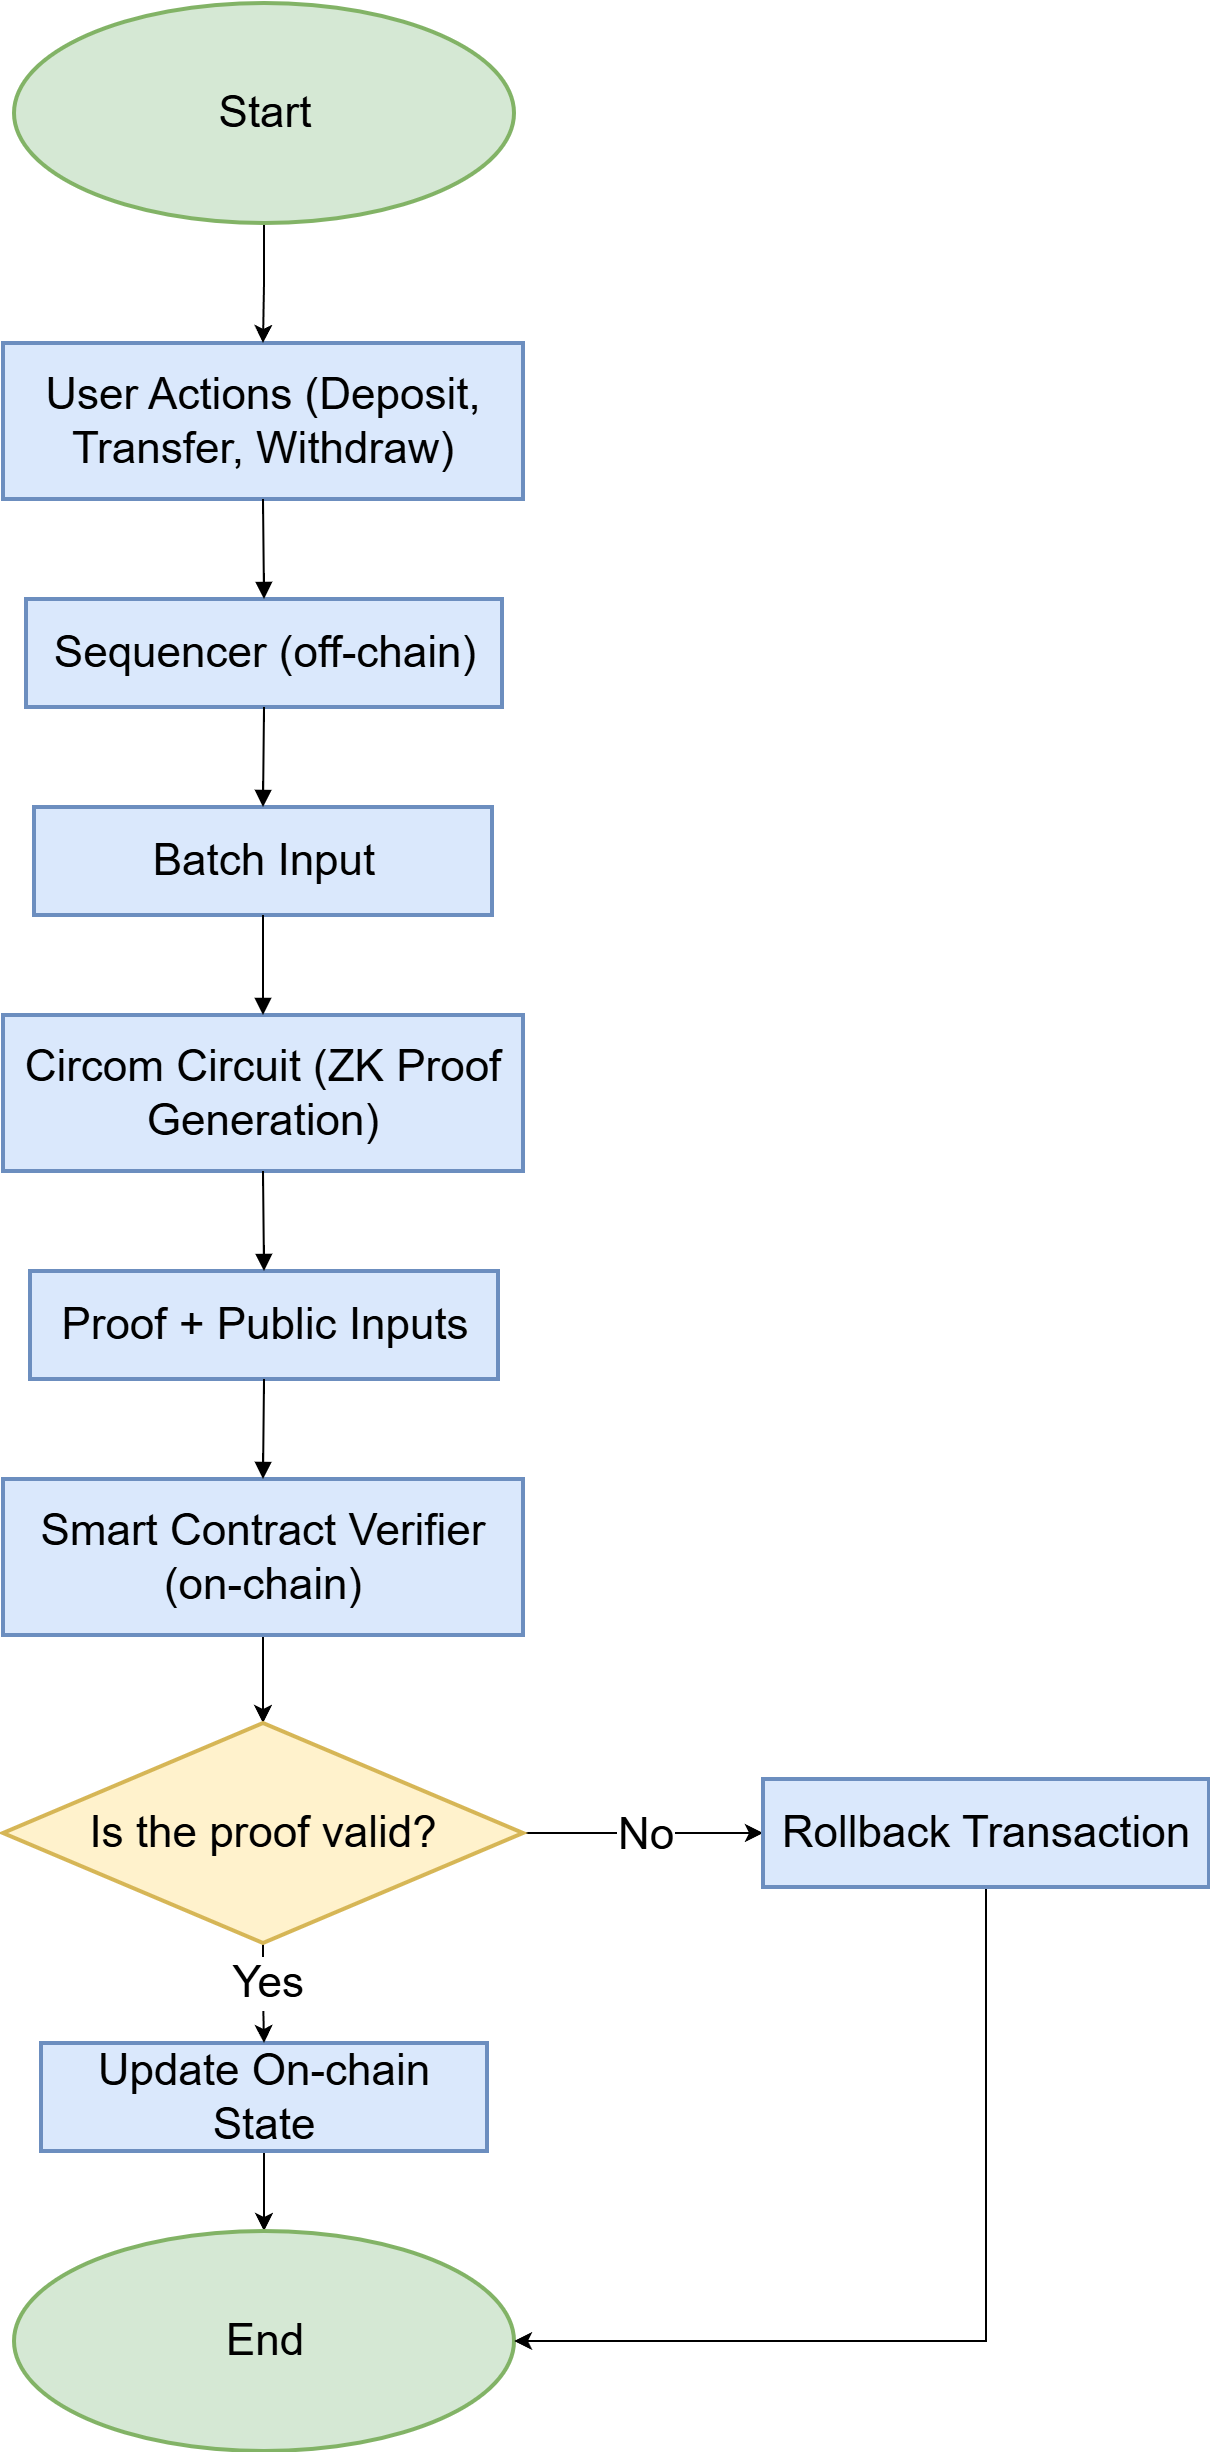
\includegraphics[width = 0.6\textwidth]{imgs/SimpleRollupBaseline.png}
    \caption{Lược đồ mô tả đơn giản hoạt động của các chức năng trong ZK-Rollup mô phỏng}
    \label{fig:chapter4-SimpleRollupBaseline}
\end{figure}

\begin{itemize}
    \item Người dùng khởi tạo một giao dịch (gửi tiền vào layer 2, chuyển tiền giữa các tài khoản, hoặc rút tiền về layer 1). Đối với các giao dịch chuyển và rút tiền, yêu cầu được gửi trực tiếp tới sequencer; đối với gửi tiền, sequencer theo dõi sự kiện từ hợp đồng thông minh layer 1 để ghi nhận. Các giao dịch sau đó được xếp hàng chờ cho đến khi đạt đến ngưỡng lô xác định.
    \item Khi lô giao dịch hoặc yêu cầu rút tiền đã đủ số lượng giao dịch và được chuẩn bị, sequencer tạo ra các đầu vào cho mạch ZK và sử dụng snarkjs để tạo ra ZKP và các tín hiệu công khai.
    \item Bằng chứng và các tín hiệu công khai được gửi tới hợp đồng thông minh tương ứng trên blockchain để xác thực.
    \item Sau khi xác nhận bằng chứng hợp lệ, hợp đồng thông minh cập nhật cây Merkle để cập nhật trạng thái trên chuỗi, trong khi giao dịch cũng được xác nhận ngoài chuỗi bởi sequencer, và được cập nhật trạng thái ngoài chuỗi.
\end{itemize}

% Quy trình chi tiết của hệ thống được minh họa trong Hình 4.2 và có thể được tóm tắt lại trong Hình 4.1 như sau. 
% Trước tiên, người dùng khởi tạo một giao dịch, có thể bao gồm việc gửi tiền vào layer 2, chuyển tiền giữa các tài khoản, hoặc rút tiền về layer 1. Đối với các giao dịch chuyển và rút tiền, yêu cầu được gửi trực tiếp đến sequencer để xử lý. Ngược lại, đối với hoạt động gửi tiền vào layer 2, sequencer sẽ theo dõi các sự kiện phát sinh từ hợp đồng thông minh trên layer 1 nhằm ghi nhận giao dịch tương ứng. Tất cả các giao dịch sau đó được xếp hàng chờ cho đến khi đạt đến ngưỡng xác định để tạo thành một lô giao dịch.

% Khi số lượng giao dịch hoặc yêu cầu rút tiền đã đạt đến ngưỡng cần thiết và sẵn sàng xử lý, sequencer tiến hành tạo các đầu vào phù hợp cho mạch ZK, đồng thời sử dụng công cụ snarkjs để tạo ra bằng chứng không kiến thức (Zero-Knowledge Proof – ZKP) cùng với các tín hiệu công khai tương ứng. Các bằng chứng và tín hiệu công khai này được gửi tới hợp đồng thông minh tương ứng trên blockchain để thực hiện bước xác thực.

% Sau khi hợp đồng thông minh xác nhận bằng chứng là hợp lệ, cây Merkle sẽ được cập nhật để phản ánh trạng thái mới trên chuỗi. Đồng thời, trạng thái ngoài chuỗi của giao dịch cũng được cập nhật bởi sequencer, đảm bảo rằng quá trình xử lý được duy trì nhất quán giữa dữ liệu on-chain và off-chain.


\begin{figure}[h]
    \centering
    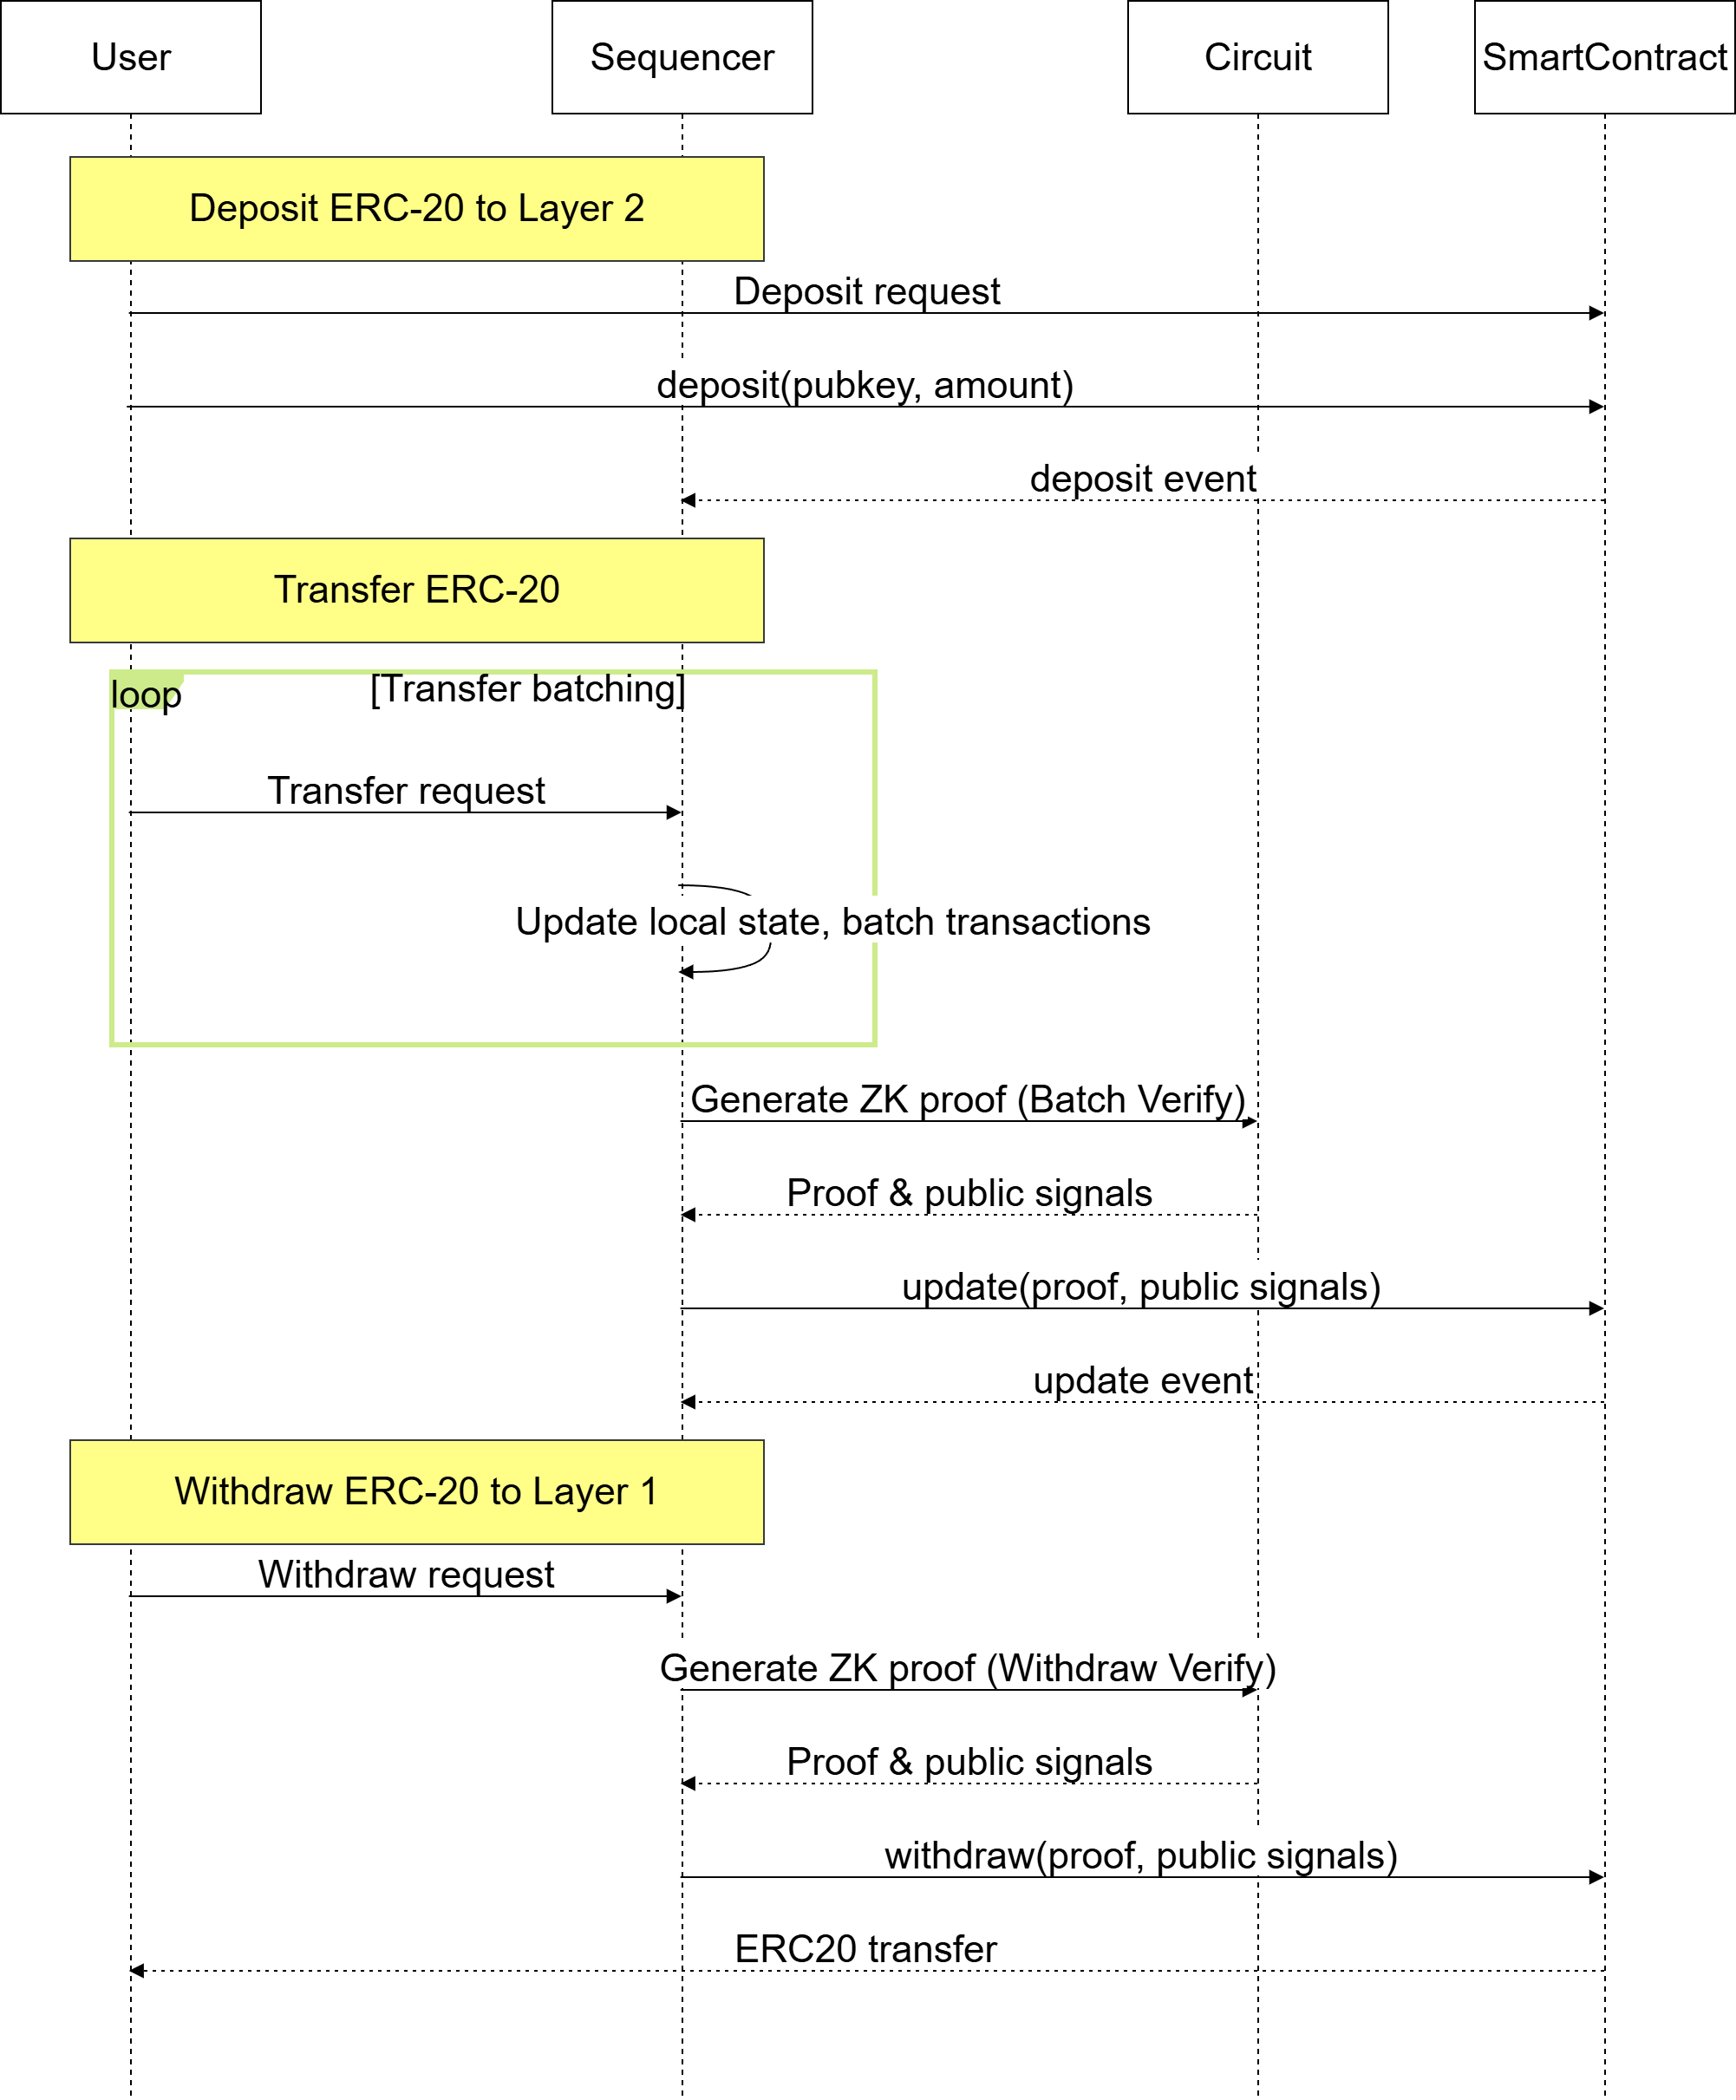
\includegraphics[width = 0.9\textwidth]{imgs/RollupBaseline.png}
    \caption{Lược đồ mô tả chi tiết hoạt động của các chức năng trong ZK-Rollup mô phỏng}
    \label{fig:chapter4-RollupBaseline}
\end{figure}
\clearpage
\section{Phương pháp đề xuất: ZK Circuit Lifecycle Strategy (ZCLS)}

Các kết quả thực nghiệm nhấn mạnh rằng thời gian biên dịch là một rào cản phát triển đáng kể cho các triển khai ZK-Rollup quy mô lớn. Mặc dù cần thiết phải sử dụng --O2 để đảm bảo sinh chứng minh hiệu quả, sự đánh đổi với thời gian biên dịch tăng lên có thể làm gián đoạn quy trình làm việc khi phát triển ứng dụng. Do đó, việc lựa chọn cờ tối ưu hóa ràng buộc của trình biên dịch mạch một cách phù hợp có vai trò quan trọng và cần được cân nhắc kĩ lưỡng. Dựa trên các phân tích thực nghiệm về tác động của các mức tối ưu hoá ràng buộc của Circom, nghiên cứu này đề xuất một phương pháp luận có cấu trúc, được gọi là ZCLS. Phương pháp ZCLS cung cấp một khung hướng dẫn cho các nhà phát triển trong việc đưa ra quyết định sáng suốt về tối ưu hóa mạch ZKP xuyên suốt các giai đoạn khác nhau của quá trình phát triển và triển khai.

\subsection{Giới thiệu về ZCLS}
ZCLS là một phương pháp tiếp cận nhằm quản lý và tối ưu hóa quá trình biên dịch mạch ZKP, từ giai đoạn thiết kế ban đầu cho đến triển khai sản phẩm. Mục tiêu của ZCLS là cân bằng giữa tốc độ phát triển (thời gian biên dịch) và hiệu suất thực thi (thời gian tạo bằng chứng), dựa trên các yêu cầu cụ thể của từng giai đoạn. ZCLS hoạt động với nhận thức rằng không có một cờ tối ưu hóa nào là ``tốt nhất'' cho mọi tình huống; thay vào đó, lựa chọn tối ưu phụ thuộc vào các yếu tố như tần suất cập nhật mạch, khối lượng bằng chứng cần tạo, và giai đoạn hiện tại của dự án.

\subsection{Các yếu tố quyết định trong ZCLS}
ZCLS xem xét ba yếu tố chính để đưa ra khuyến nghị về cờ tối ưu hóa:
\begin{enumerate}
    \item \textbf{Giai đoạn Phát triển (Development Stage)}

    Đây là yếu tố đầu tiên và quan trọng nhất, xác định ưu tiên chính của quá trình tối ưu hóa:
    \begin{itemize}
        \item \textbf{Phát triển và Thử nghiệm (Development and Testing):} Trong giai đoạn này, mạch ZKP thường xuyên được thay đổi, bổ sung tính năng, và gỡ lỗi. Ưu tiên hàng đầu là tốc độ biên dịch nhanh để rút ngắn chu kỳ phản hồi và tăng hiệu quả làm việc của nhà phát triển. Hiệu suất tạo bằng chứng vẫn quan trọng cho việc kiểm thử, nhưng không phải là yếu tố quyết định tuyệt đối.
        \item \textbf{Triển khai Thực tế (Production Deployment): }Khi mạch đã ổn định và sẵn sàng cho môi trường sản phẩm, ưu tiên chuyển sang hiệu suất tạo bằng chứng tối đa và ổn định. Tần suất cập nhật mạch giảm đáng kể, do đó thời gian biên dịch dài hơn có thể được chấp nhận. 
        \item \textbf{Trường Hợp Đặc Biệt (Gỡ Lỗi - Debugging): }Trong các tình huống cần gỡ lỗi sâu hoặc kiểm tra nhanh các phần nhỏ của mạch, tốc độ biên dịch là yếu tố quan trọng nhất, thậm chí hy sinh hiệu suất tạo bằng chứng.
    \end{itemize}
    
    \item \textbf{Tần suất cập nhật mạch (Circuit Update Frequency)}

    ``Tần suất cập nhật mạch'' đề cập đến số lần cập nhật mạch trong quá trình phát triển, tức là số lần nhà phát triển thay đổi mã nguồn của mạch và cần biên dịch lại. Yếu tố này ảnh hưởng trực tiếp đến thời gian chờ đợi của nhà phát triển. Tần suất cập nhật mạch càng cao, yêu cầu về thời gian biên dịch càng nhanh để không làm gián đoạn quy trình làm việc. Các ngưỡng định lượng được gợi ý giúp nhà phát triển tham chiếu và sử dụng khung hướng dẫn một cách dễ dàng hơn.

    % Dựa trên dữ liệu benchmark của chúng tôi (đặc biệt tại lô giao dịch 64, đại diện cho kịch bản tải cao nhất trong thử nghiệm hiện tại), chúng tôi định lượng tác động của tần suất cập nhật mạch đến yêu cầu về thời gian biên dịch như sau:

    \begin{itemize}
        \item \textbf{Cao (High Frequency):} Tần suất này thường xuất hiện ở giai đoạn phát triển và thử nghiệm lặp lại, nơi các thay đổi mạch diễn ra thường xuyên (\textit{ví dụ:} nhiều lần trong một giờ hoặc một ngày). Trong giai đoạn này, thời gian biên dịch của mỗi lần thay đổi là yếu tố quan trọng. Yều cầu về thời gian biên dịch của giai đoạn này là \textit{nhanh}. \textbf{Ngưỡng định lượng đề xuất:} Từ 10 - 50 lần/ngày.
        % Dựa trên dữ liệu của chúng tôi, thời gian biên dịch của --O0 (\textasciitilde 46 giây) và --O1 (\textasciitilde 64 giây) tại kích thước lô 64 là chấp nhận được cho các vòng lặp phát triển nhanh. Thời gian biên dịch của --O2 (\textasciitilde 122 giây) có thể gây ra sự chậm trễ đáng kể.
        
        % \textbf{Ngưỡng định lượng:} Yêu cầu thời gian biên dịch nhanh -- Chọn dưới 65 giây cho kích thước lô 64 (sử dụng --O0 hoặc --O1). 

        \item \textbf{Thấp (Low Frequency):} Áp dụng cho các mạch đã ổn định, hiếm khi được cập nhật, chỉ khi có các bản nâng cấp lớn, vá lỗi bảo mật nghiêm trọng hoặc thay đổi giao thức cốt lõi. Trong trường hợp này, yêu cầu về thời gian biên dịch mạch là \textit{không quan trọng}. \textbf{Ngưỡng định lượng đề xuất:} dưới 1 lần/tuần (\textit{ví dụ:} 1 lần/tháng, 1 lần/quý, hoặc ít hơn).
        % Trong trường hợp này, thời gian biên dịch dài hơn của --O2 là chấp nhận được vì nó không ảnh hưởng đáng kể đến năng suất tổng thể.

        % \textbf{Ngưỡng định lượng:} Yêu cầu thời gian biên dịch chấp nhận được -- trên 65 giây cho Batch Size 64 (sử dụng --O2).

        \item \textbf{Rất Cao -- Dùng khi gỡ lỗi (Very High Frequency for Debugging):} Khi tốc độ biên dịch là ưu tiên tuyệt đối để gỡ lỗi nhanh, ngay cả khi hiệu suất tạo bằng chứng không tối ưu. Trong trường hợp này, yêu cầu về thời gian biên dịch sẽ là \textit{rất nhanh}. \textbf{Ngưỡng định lượng đề xuất:} Trên 50 lần/ngày (hoặc nhiều lần mỗi giờ).
        % Điều này chỉ có thể đạt được với --O0.

        % \textbf{Ngưỡng định lượng:} Yêu cầu thời gian biên dịch tối thiểu -- dưới 50 giây cho kích thước lô 64 (sử dụng --O0).
    \end{itemize}
    
    \item \textbf{Khối lượng tạo bằng chứng (Proof Generation Volume)}

    ``Khối lượng tạo bằng chứng'' đề cập đến số lượng bằng chứng dự kiến sẽ tạo ra để kiểm tra hệ thống, tức là quy mô của các bài kiểm tra hoặc số lượng giao dịch cần được xử lý trong một lô để xác minh. Yếu tố này ảnh hưởng trực tiếp đến thời gian tạo bằng chứng và khả năng mở rộng của hệ thống.

    % Dựa trên dữ liệu benchmark của chúng tôi (tại kích thước lô 64), chúng tôi định lượng tác động của khối lượng tạo bằng chứng đến yêu cầu về thời gian tạo bằng chứng như sau:

    \begin{itemize}
    
    \item \textbf{Cao (High Volume):} Khối lượng này sẽ xảy ra với các trường hợp cần tạo bằng chứng cho các lô giao dịch lớn hoặc khi cần tạo bằng chứng liên tục để kiểm thử thông lượng của hệ thống. Đây là nơi tối ưu hóa thời gian tạo bằng chứng (như --O2) trở nên cực kỳ quan trọng. Yêu cầu về thời gian tạo bằng chứng ở trường hợp này sẽ là \textit{nhanh}. \textbf{Ngưỡng định lượng đề xuất:} 
    Trên 100 bằng chứng/ngày.
    
    % Dựa trên dữ liệu của chúng tôi, thời gian tạo bằng chứng của --O2 (\textasciitilde 29 giây) và --O1 (\textasciitilde 37 giây) tại kích thước lô 64 là phù hợp cho các kịch bản này.

    % \textbf{Ngưỡng định lượng:} Yêu cầu thời gian tạo bằng chứng nhanh -- dưới 40 giây cho kích thước lô 64 (sử dụng --O1 hoặc --O2).

    \item \textbf{Thấp (Low Volume):} Ám chỉ các trường hợp cần tạo bằng chứng không thường xuyên hoặc cho các lô giao dịch nhỏ trong quá trình kiểm thử. Yêu cầu về thời gian tạo bằng chứng của trường hợp này sẽ là \textit{trung bình}. \textbf{Ngưỡng định lượng đề xuất:} Từ 50 - 100 bằng chứng/ngày.
    
    % Thời gian tạo bằng chứng dài hơn của --O0 (\textasciitilde75 giây) là chấp nhận được.

    % \textbf{Ngưỡng định lượng:} Yêu cầu thời gian tạo bằng chứng chấp nhận được -- trên 40 giây cho kích thước lô 64 (sử dụng --O0).

    \item \textbf{Rất Thấp (Very Low Volume for Debugging):} Khi thời gian tạo bằng chứng không phải là mối quan tâm, ưu tiên tuyệt đối sẽ dành cho tốc độ biên dịch, ngay cả khi hiệu suất tạo bằng chứng không tối ưu. Điều này tương ứng với hiệu suất của --O0 với yêu cầu về thời gian biên dịch là \textit{rất nhanh}. \textbf{Ngưỡng định lượng đề xuất:} Dưới 1 bằng chứng/giờ (\textit{ví dụ:} 1 bằng chứng/ngày hoặc ít hơn).

    % \textbf{Ngưỡng định lượng:} Yêu cầu thời gian tạo bằng chứng không quan trọng -- trên 70 giây cho kích thước lô 64 (sử dụng --O0).
    \end{itemize}
\end{enumerate}

\subsection{Bảng và khung khuyến nghị ZCLS}
Dựa trên các yếu tố định tính và yêu cầu hiệu suất tương ứng, bảng khuyến nghị ZCLS được trình bày trong bảng \ref{tab:optimization_flag_selection} và hình \ref{fig:chapter4-FrameworkCircom}.

\begin{table}[h]
    \centering
    \caption{Các mức tối ưu hóa trình biên dịch Circom được khuyến nghị dựa trên giai đoạn phát triển, tần suất cập nhật mạch và khối lượng bằng chứng được tạo.}
    \resizebox{\textwidth}{!}{%
    \begin{tabular}{|l|l|l|l|}
        \hline
        \textbf{Giai Đoạn Phát Triển} & \textbf{Tần Suất Cập Nhật Mạch} & \textbf{Khối Lượng Tạo Bằng Chứng} & \textbf{Cờ Được Khuyến Nghị} \\
        \hline
        Trường Hợp Đặc Biệt (Gỡ Lỗi) & Rất Cao (Thường Xuyên) & Rất Thấp & --O0 \\
        Phát Triển, Thử Nghiệm & Cao & Thấp & --O1 \\
        Phát Triển, Thử Nghiệm & Cao & Cao & --O1 \\
        Triển Khai Thực Tế & Thấp & Cao & --O2 \\
        Triển Khai Thực Tế & Thấp & Thấp & --O2 \\
        \hline
    \end{tabular}
    }
    \label{tab:optimization_flag_selection}
\end{table}

% ver 1
%\clearpage
% \begin{figure}[h] % 'h' để đặt ảnh gần vị trí lệnh
%     \centering % Căn giữa ảnh
%     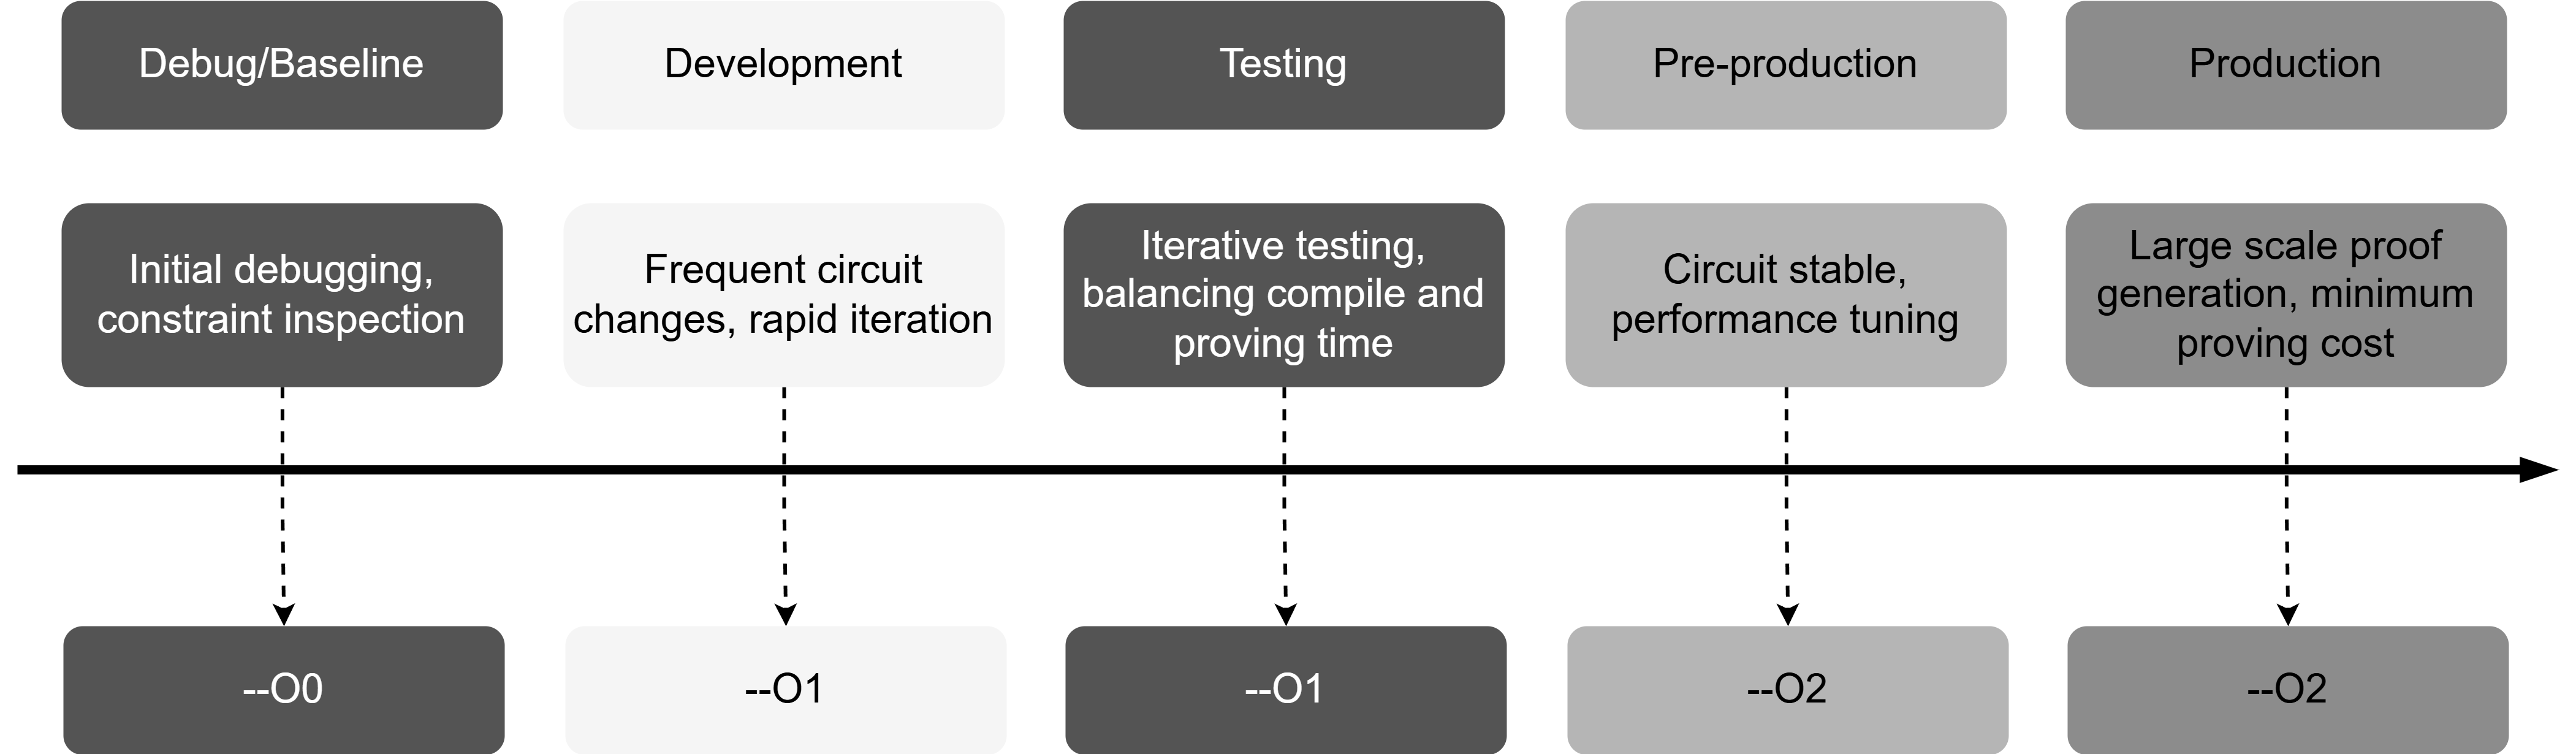
\includegraphics[width=\textwidth]{imgs/framework.png}
%     \caption{Khung chọn cờ tối ưu hóa trình biên dịch Circom dựa trên giai đoạn phát triển, tần suất cập nhật mạch và khối lượng tạo bằng chứng}
%     \label{fig:chapter4-framework}
% \end{figure}

% ver 2
% \begin{figure}[h] % 'h' để đặt ảnh gần vị trí lệnh
%     \centering % Căn giữa ảnh
%     \rotatebox{90}{
%     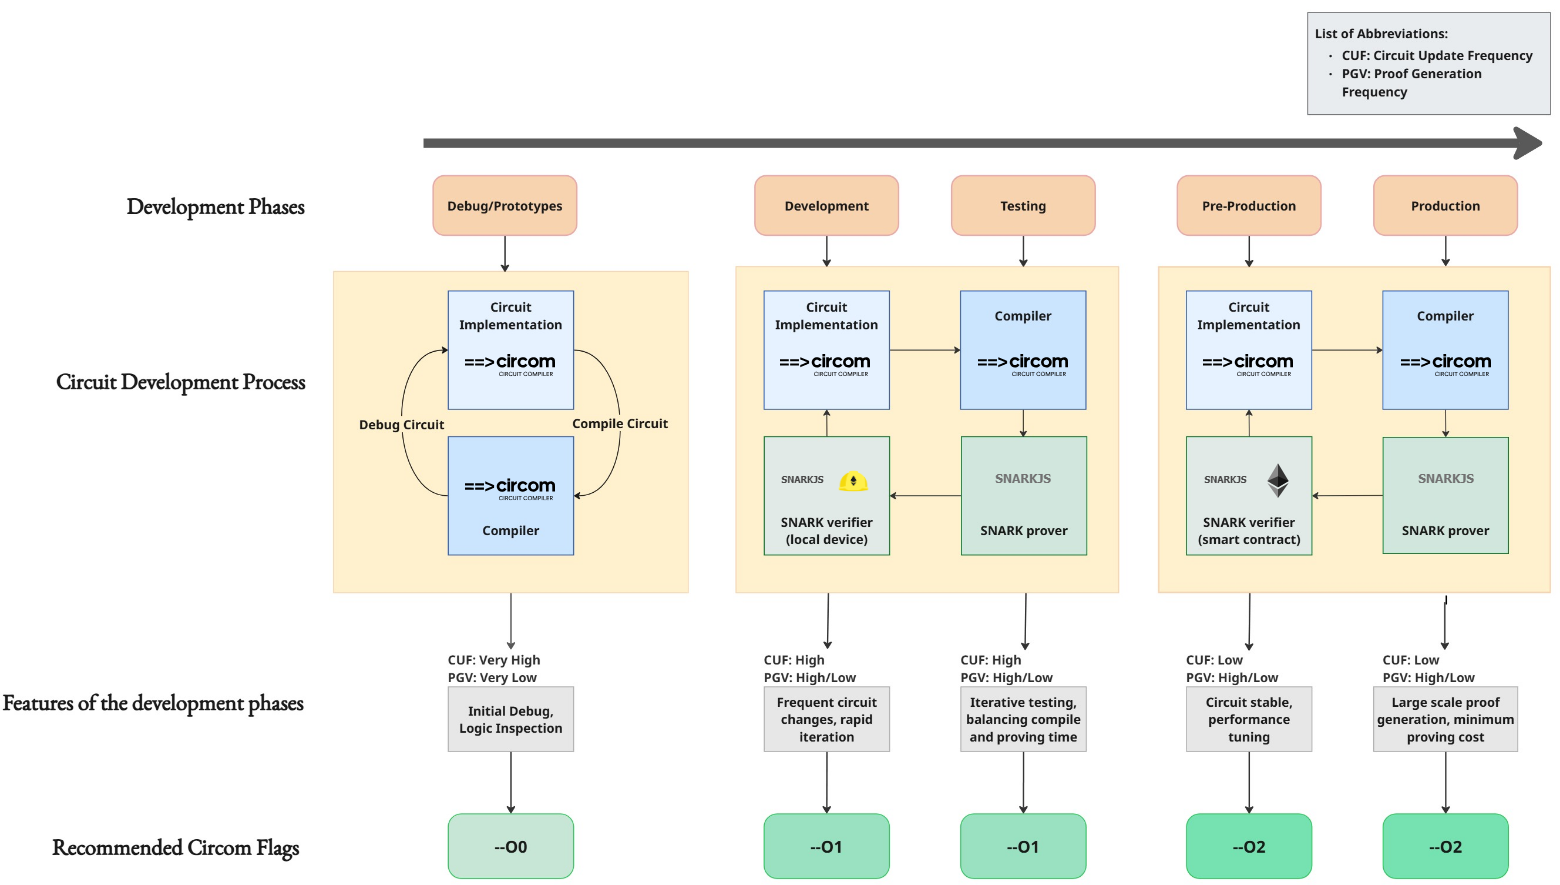
\includegraphics[height=0.7\textwidth]{imgs/FrameworkCircom.drawio.png}}
%     \caption{Khung chọn cờ tối ưu hóa trình biên dịch Circom dựa trên giai đoạn phát triển, tần suất cập nhật mạch và khối lượng tạo bằng chứng}
%     \label{fig:chapter4-FrameworkCircom1}
% \end{figure}

% ver 3
% \begin{figure}[h] % 'h' để đặt ảnh gần vị trí lệnh
%     \centering % Căn giữa ảnh
%     \rotatebox{90}{
%     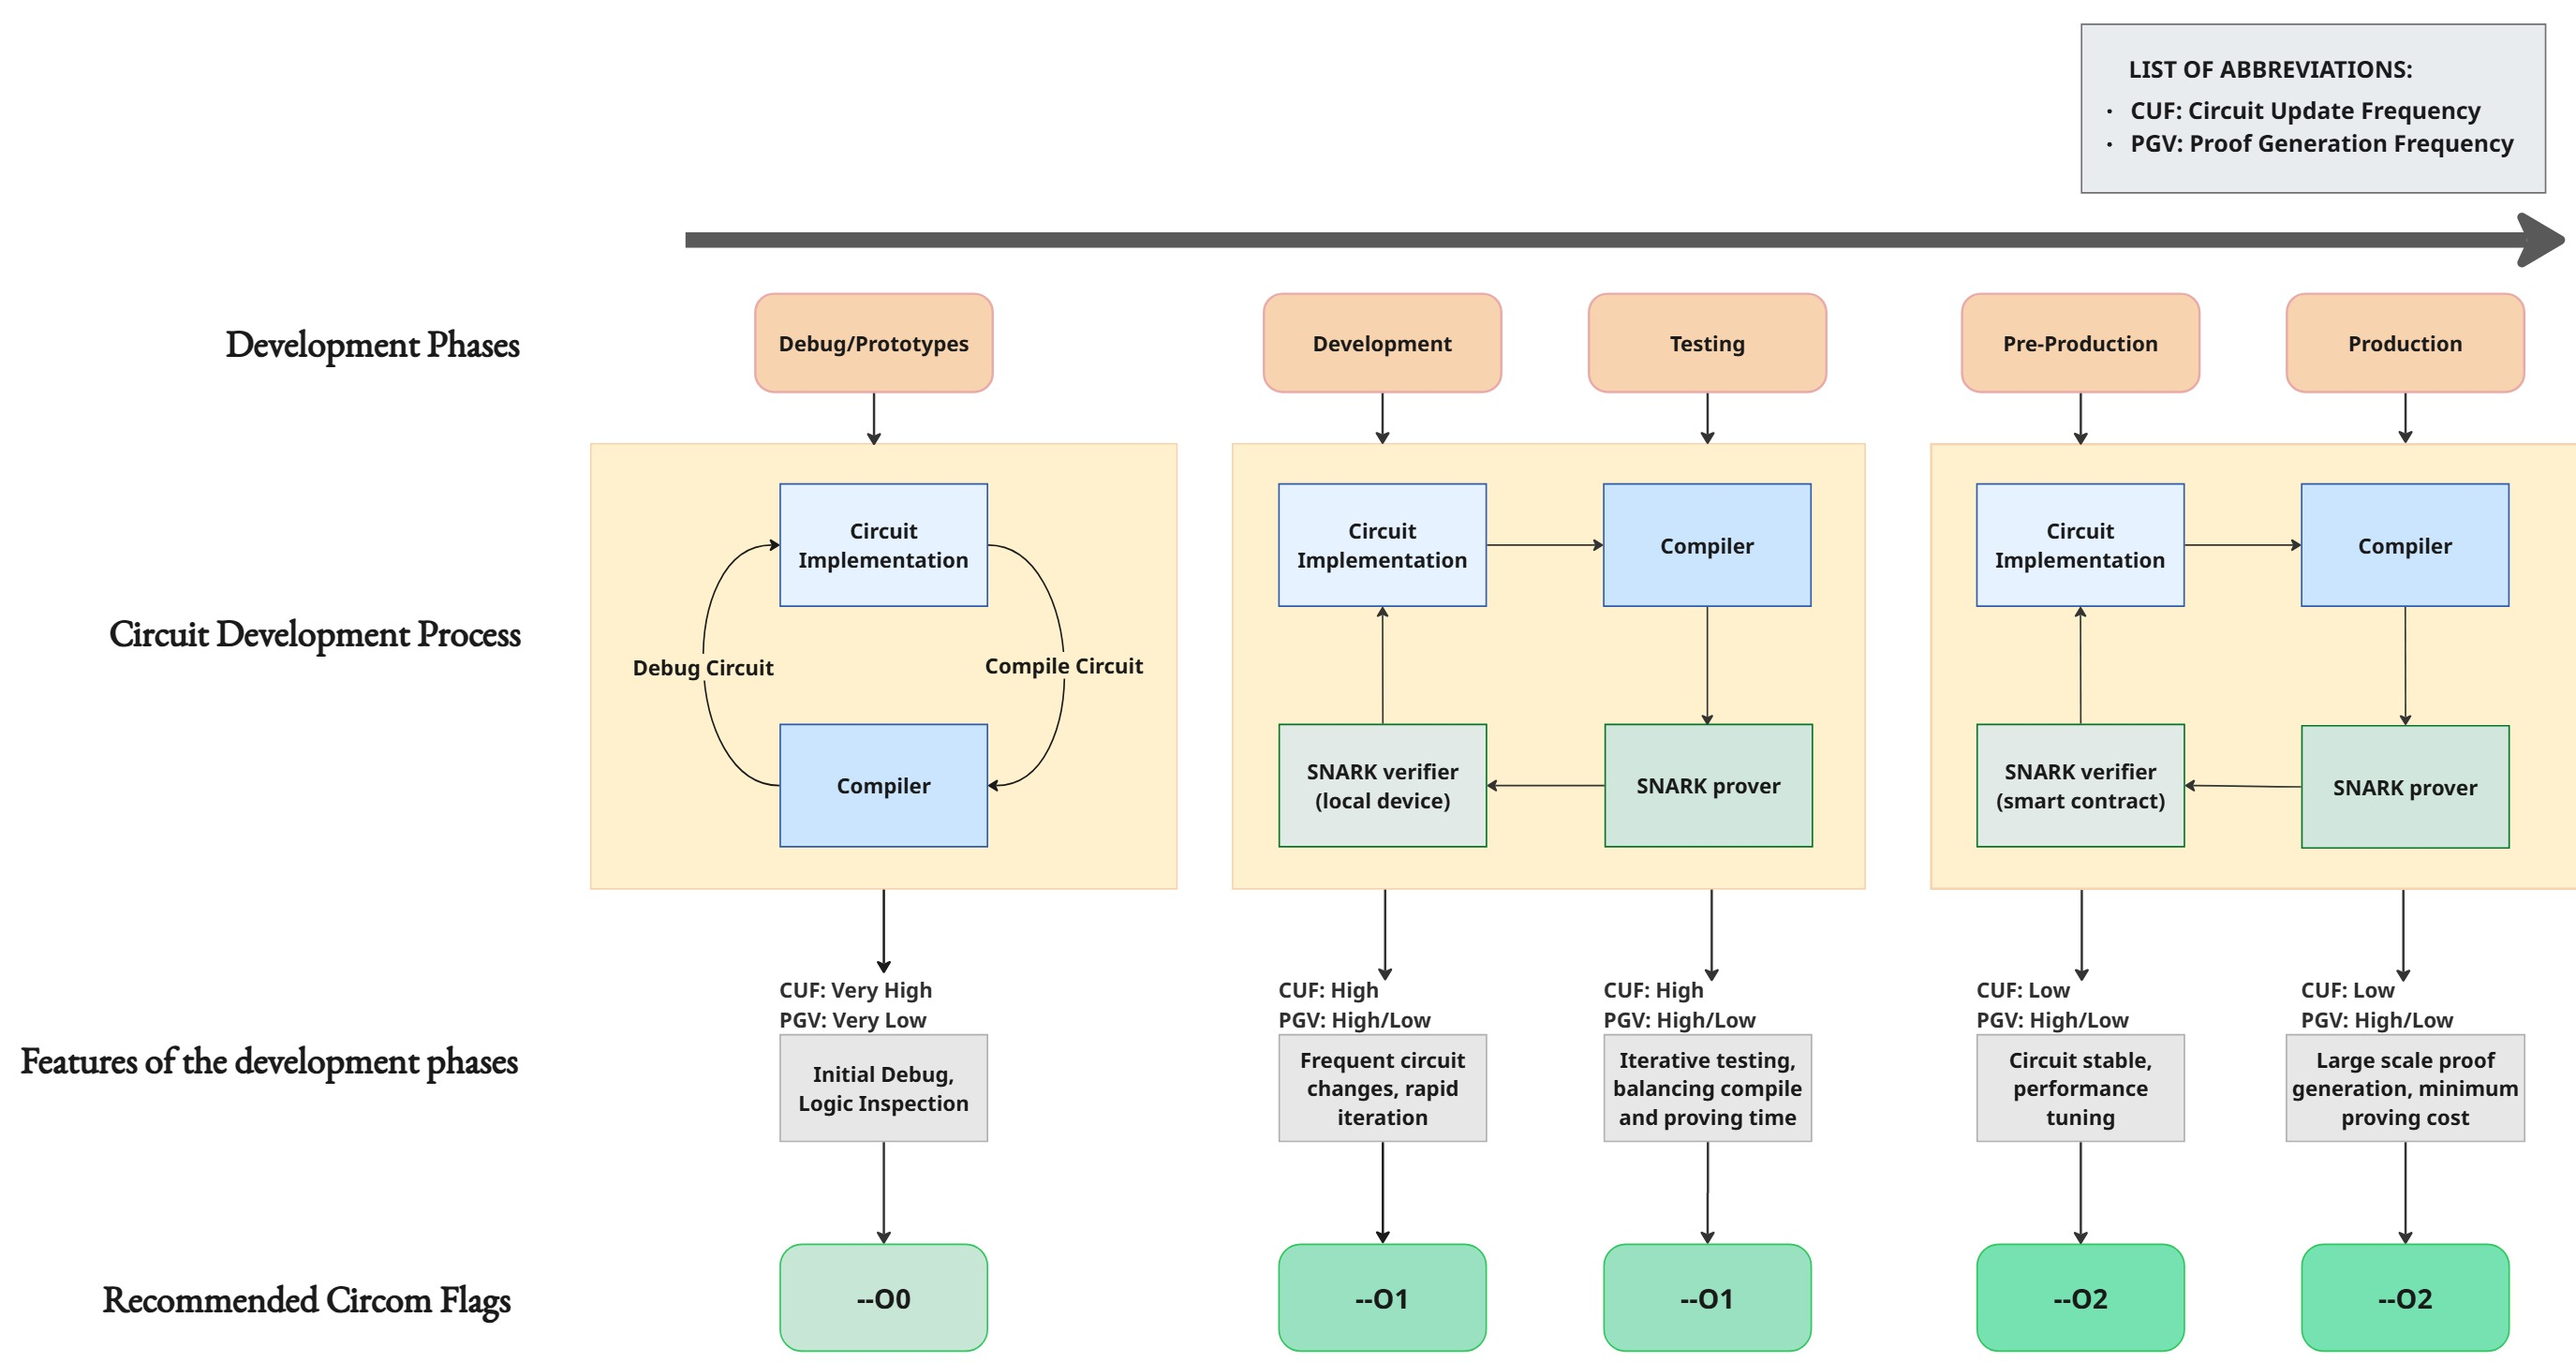
\includegraphics[height=0.7\textwidth]{imgs/FrameworkCircom.jpg}}
%     \caption{Khung chọn cờ tối ưu hóa trình biên dịch Circom dựa trên giai đoạn phát triển, tần suất cập nhật mạch và khối lượng tạo bằng chứng}
%     \label{fig:chapter4-FrameworkCircom}
% \end{figure}

% \begin{figure}[h] % 'h' để đặt ảnh gần vị trí lệnh
%     \centering % Căn giữa ảnh
%     \rotatebox{90}{
%     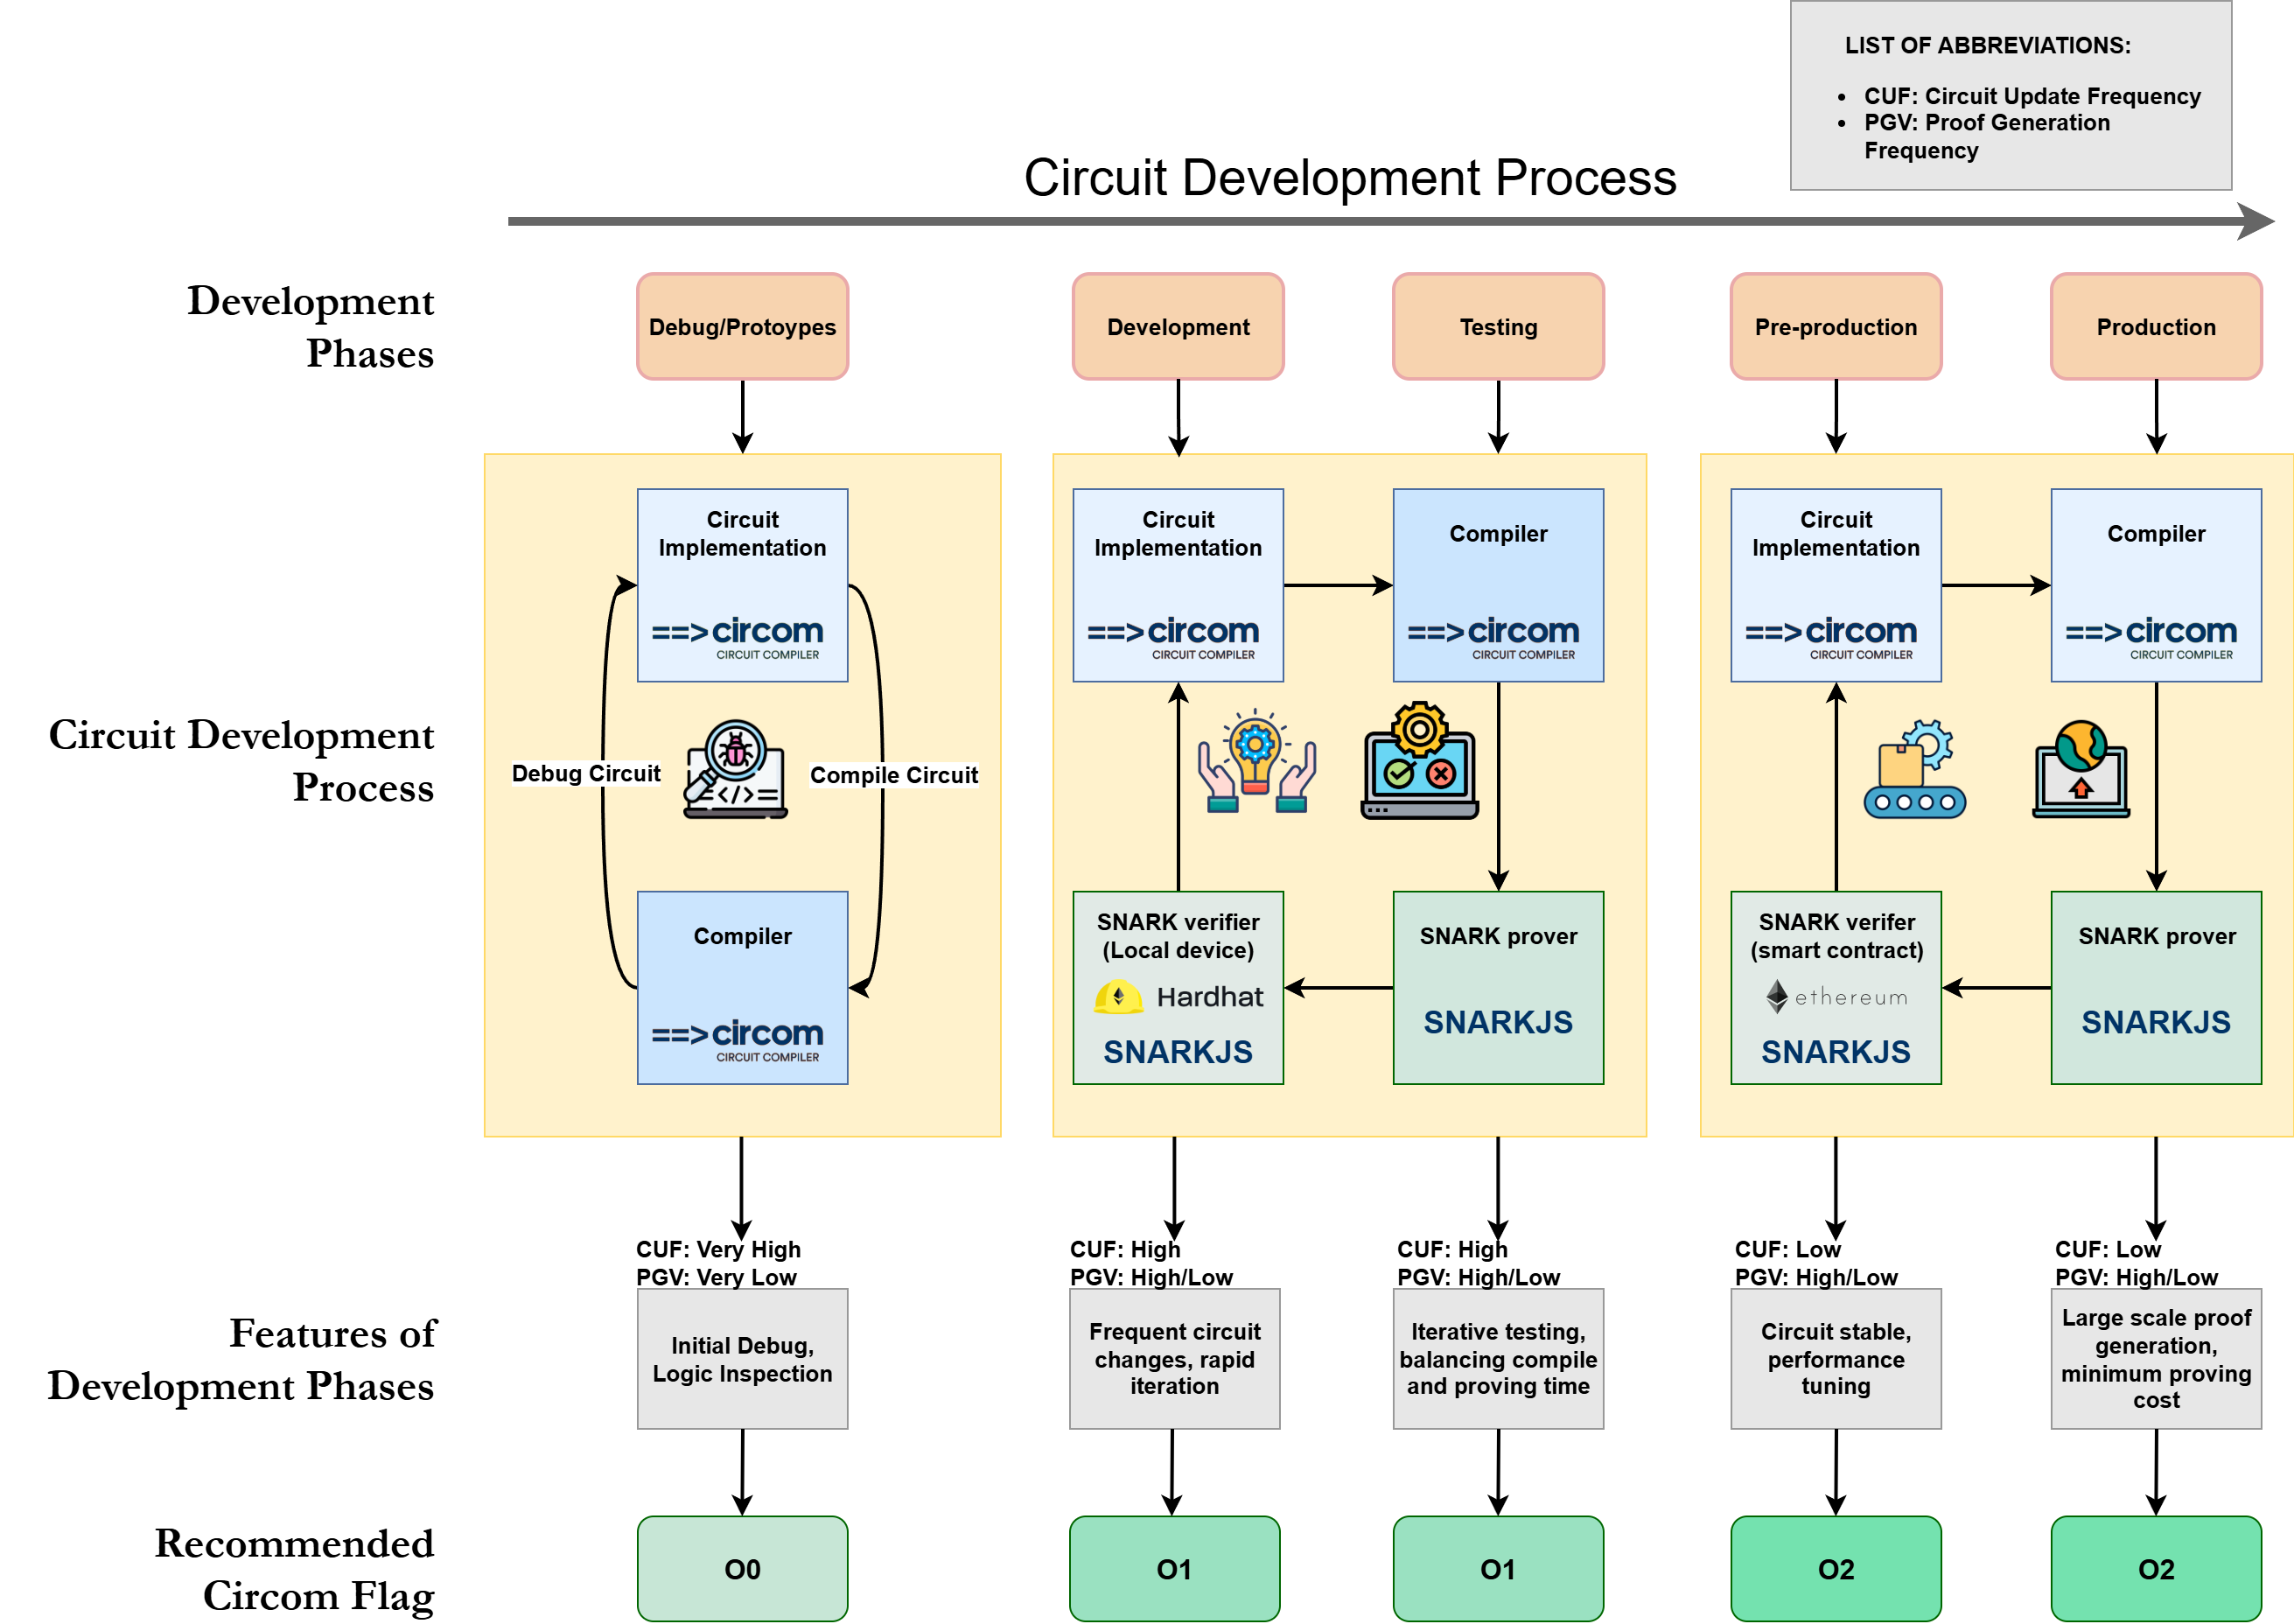
\includegraphics[height=0.9\textwidth]{imgs/FlagSelection.png}}
%     \caption{Khung chọn cờ tối ưu hóa trình biên dịch Circom dựa trên giai đoạn phát triển, tần suất cập nhật mạch và khối lượng tạo bằng chứng}
%     \label{fig:chapter4-FrameworkCircom}
% \end{figure}

Các khuyến nghị trong khung và bảng trên được xây dựng dựa trên sự đánh đổi giữa thời gian biên dịch và thời gian tạo bằng chứng, được định lượng từ dữ liệu thực nghiệm của nghiên cứu (đặc biệt tại kích thước lô 64, đại diện cho kịch bản lô cao nhất trong thử nghiệm hiện tại). Dưới đây là phần giải thích cho từng trường hợp cụ thể:

\begin{enumerate}
    \item \textbf{Phát Triển, Thử Nghiệm (Development, Testing):}
    \begin{itemize}
        \item \textbf{Tần Suất Cập Nhật Mạch: Cao} -- \textbf{Yêu cầu thời gian biên dịch nhanh}:
        \begin{itemize}
            \item \textbf{Khối Lượng Tạo Bằng Chứng: Thấp} -- \textbf{Yêu cầu thời gian tạo bằng chứng trung bình}: Trong kịch bản này, ưu tiên hàng đầu là tốc độ biên dịch để nhà phát triển có thể lặp lại quá trình biên dịch nhanh chóng. --O1 được khuyến nghị vì nó cung cấp thời gian biên dịch nhanh (\textasciitilde 64s) và thời gian tạo bằng chứng chấp nhận được (\textasciitilde 37s), là sự cân bằng tốt nhất. --O0 biên dịch nhanh hơn nhưng thời gian tạo bằng chứng quá chậm (\textasciitilde 75s) có thể làm chậm quá trình kiểm thử, trong khi --O2 có thời gian biên dịch quá dài (\textasciitilde 122s).
            \item \textbf{Khối Lượng Tạo Bằng Chứng: Cao} -- \textbf{Yêu cầu thời gian tạo bằng chứng nhanh}: Ngay cả khi cần tạo bằng chứng nhanh cho các bài kiểm thử tải cao, --O1 vẫn là lựa chọn cân bằng. Nó cung cấp thời gian biên dịch nhanh (\textasciitilde 64s) và thời gian tạo bằng chứng đủ nhanh (\textasciitilde 36s) để kiểm thử các kịch bản tải cao mà không phải chịu chi phí biên dịch quá lớn của --O2. Điều này cho phép nhà phát triển nhanh chóng kiểm tra hiệu suất mạch mà không bị cản trở bởi thời gian biên dịch kéo dài.
        \end{itemize}
    \end{itemize}

    \item \textbf{Triển Khai Thực Tế (Production Deployment):}
    \begin{itemize}
        \item \textbf{Tần Suất Cập Nhật Mạch: Thấp} -- \textbf{Yêu cầu thời gian biên dịch trung bình}: Khi mạch đã ổn định và sẵn sàng cho môi trường sản phẩm, tần suất cập nhật mạch giảm đáng kể, do đó thời gian biên dịch dài hơn của --O2 (\textasciitilde 122s) là chấp nhận được.
        \begin{itemize}
            \item \textbf{Khối Lượng Tạo Bằng Chứng: Cao} -- \textbf{Yêu cầu thời gian tạo bằng chứng nhanh:} Đây là trường hợp phổ biến nhất trong môi trường triển khai thực tế của ZK-Rollup, nơi cần xử lý lượng lớn giao dịch. Ưu tiên hàng đầu là hiệu suất tạo bằng chứng tối đa để xử lý thông lượng giao dịch. --O2 cung cấp thời gian tạo bằng chứng nhanh nhất (\textasciitilde 28s), vượt trội so với --O1 (\textasciitilde 37s) và --O0 (\textasciitilde 75s). Việc lựa chọn --O2 là hợp lý để đảm bảo hiệu suất tối ưu và khả năng mở rộng trong tương lai.
            \item \textbf{Khối Lượng Tạo Bằng Chứng: Thấp -- Yêu cầu thời gian tạo bằng chứng \textbf{nhanh}:} Mặc dù khối lượng bằng chứng thấp, --O2 vẫn là lựa chọn tốt nhất. Trong môi trường sản phẩm, ngay cả khi khối lượng bằng chứng không quá cao, việc sử dụng cờ tối ưu hóa mang lại hiệu suất tạo bằng chứng tốt nhất vẫn là ưu tiên để đảm bảo tính ổn định và hiệu quả tổng thể của hệ thống. Mặc dù khối lượng tạo bằng chứng là thấp có thể ngụ ý rằng thời gian tạo bằng chứng có thể là trung bình trong các giai đoạn khác, nhưng trong môi trường triển khai thực tế, mục tiêu luôn là tối ưu hóa hiệu suất. Do đó, --O2 vẫn là lựa chọn ưu tiên để đảm bảo thời gian tạo bằng chứng nhanh nhất có thể, ngay cả khi khối lượng bằng chứng không quá lớn. Điều này phản ánh thực tế rằng trong môi trường sản phẩm, mọi cải thiện về hiệu suất đều có giá trị.
        \end{itemize}
    \end{itemize}

    \item \textbf{Trường Hợp Đặc Biệt (Gỡ Lỗi - Debugging):}
    \begin{itemize}
        \item \textbf{Tần Suất Cập Nhật Mạch: Rất Cao (Thường Xuyên)} -- \textbf{Yêu cầu thời gian biên dịch rất nhanh}: Khi gỡ lỗi, mục tiêu là biên dịch và kiểm tra mạch nhanh nhất có thể. --O0 là lựa chọn duy nhất vì nó có thời gian biên dịch nhanh nhất (\textasciitilde 46s), cho phép vòng lặp gỡ lỗi nhanh chóng.
        \begin{itemize}
            \item \textbf{Khối Lượng Tạo Bằng Chứng: Rất Thấp -- Yêu cầu thời gian tạo bằng chứng \textbf{không quan trọng}:} Trong quá trình gỡ lỗi, nhà phát triển thường không cần tạo bằng chứng mà chỉ cần biên dịch để kiểm tra tính đúng đắn của mạch. Do đó, thời gian tạo bằng chứng chậm của --O0 (\textasciitilde 75s) là hoàn toàn chấp nhận được.
            
        \end{itemize}
    \end{itemize}
    
\end{enumerate}

\subsection{Quy trình áp dụng ZCLS}
Để áp dụng ZCLS trong thực tế, nhà phát triển có thể tuân theo các bước sau:

\begin{enumerate}
    \item \textbf{Xác định Giai đoạn Phát triển hiện tại:} Dự án đang ở giai đoạn Phát triển và Thử nghiệm, Triển khai Thực tế, hay Gỡ lỗi?

    \item \textbf{Đánh giá Tần suất cập nhật mạch:} Xác định liệu bạn đang cập nhật mạch "Cao", "Thấp", hay "Rất Cao".

    \item \textbf{Đánh giá Khối lượng tạo bằng chứng:} Xác định liệu bạn cần tạo bằng chứng với "Khối lượng Cao", "Thấp", hay "Rất Thấp".

    \item \textbf{Tham chiếu Bảng khuyến nghị ZCLS:} Dựa trên các đánh giá ở bước 1, 2, 3, tra cứu bảng khuyến nghị để tìm cờ tối ưu hóa phù hợp.

    \item \textbf{Thực hiện hiệu chỉnh (nếu cần):} Nếu nhà phát triển đang làm việc với một mạch hoặc môi trường có quy mô khác biệt đáng kể so với dữ liệu thực nghiệm của nghiên cứu này, nhà phát triển có thể xác định mối ưu tiên về ``Tần suất cập nhật mạch'', ``Khối lượng tạo bằng chứng'' và chọn cờ cho phù hợp với môi trường cụ thể thực tế. Bảng gợi ý cách chọn cờ tối ưu Circom vẫn có giá trị trong trường hợp này.
    \item \textbf{Lặp lại quá trình trên:} ZCLS là một chu trình liên tục. Khi dự án chuyển sang giai đoạn khác hoặc các yêu cầu thay đổi, các nhà phát triển nên lặp lại quy trình đánh giá để điều chỉnh cờ tối ưu hóa cho phù hợp.
\end{enumerate}

Phương pháp ZCLS sẽ giúp các nhà phát triển đưa ra quyết định tối ưu hóa một cách có căn cứ, từ đó góp phần hỗ trợ nâng cao hiệu quả phát triển và hiệu suất của các ứng dụng sử dụng ZKP như ZK-Rollup.

\clearpage

\begin{figure}[h] % 'h' để đặt ảnh gần vị trí lệnh
    \centering % Căn giữa ảnh
    \rotatebox{90}{
    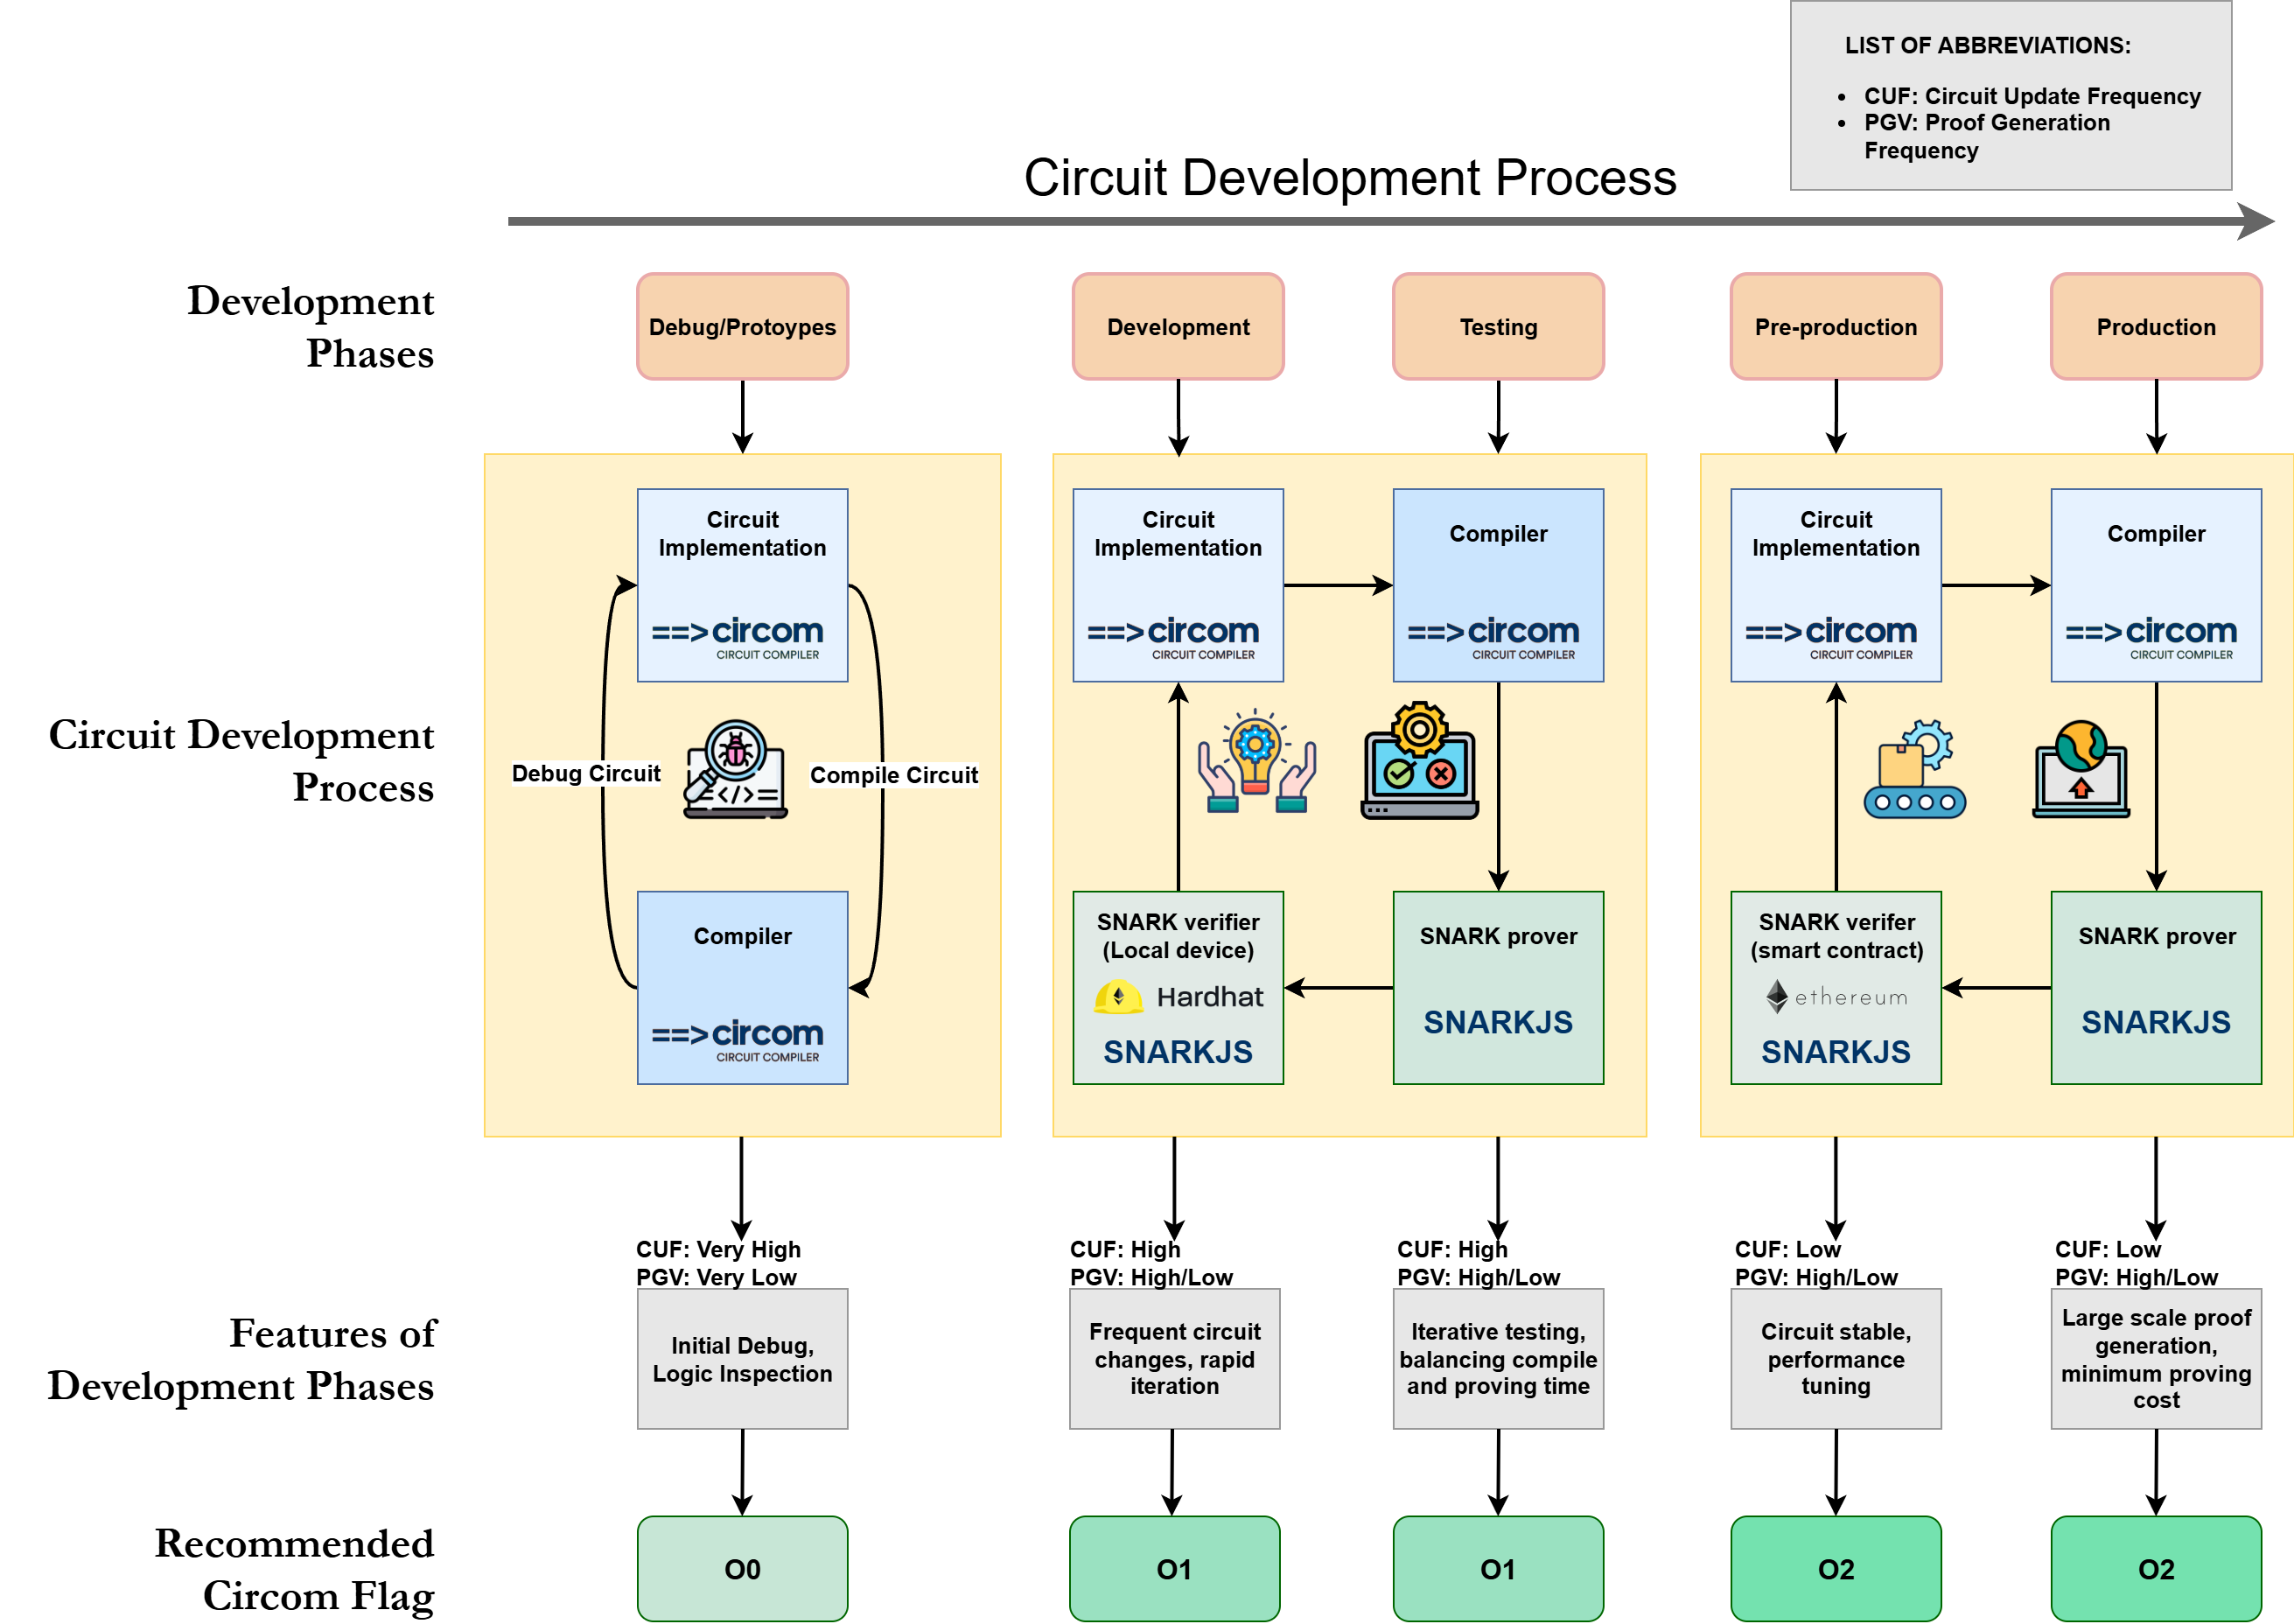
\includegraphics[height=0.9\textwidth]{imgs/FlagSelection.png}}
    \caption{Khung chọn cờ tối ưu hóa trình biên dịch Circom dựa trên giai đoạn phát triển, tần suất cập nhật mạch và khối lượng tạo bằng chứng}
    \label{fig:chapter4-FrameworkCircom}
\end{figure}
\clearpage

\section{CirMetrics: Công cụ phân tích và quản lí mạch ZKP}
\subsection{Giới thiệu}
CirMetrics là một ứng dụng hỗ trợ phát triển mạch ZKP, được em xây dựng từ nhu cầu thực tế trong việc tối ưu hóa hiệu suất biên dịch và tạo bằng chứng. Xuất phát từ nghiên cứu về chiến lược tối ưu hóa trong sử dụng trình biên dịch Circom, CirMetrics được phát triển nhằm mang lại một quy trình đánh giá hiệu quả, chính xác và trực quan hơn cho các nhà phát triển ZKP.

Ứng dụng này giúp người dùng theo dõi các thông số quan trọng trong quá trình biên dịch và tạo bằng chứng, bao gồm số lượng constraint theo từng loại, thời gian biên dịch và thời gian tạo proof. Tất cả được hiển thị bằng biểu đồ trực quan, giúp nhà phát triển dễ dàng nhận diện các vấn đề về hiệu năng và xu hướng thay đổi trong quá trình phát triển mạch.

Điểm đặc biệt của CirMetrics chính là khả năng mở rộng, hướng tới việc tích hợp các gợi ý tối ưu hóa tự động dựa trên giai đoạn phát triển của dự án. Điều này giúp các nhà phát triển Circom lựa chọn chiến lược biên dịch phù hợp, giảm chi phí tạo bằng chứng và tối ưu hóa quy trình từ nguyên mẫu đến sản phẩm hoàn chỉnh.
\subsection{Phân tích thiết kế}
Công cụ CirMetrics được thiết kế để phục vụ trực tiếp cho các nhà phát triển ứng dụng ZKP. Công cụ này được thiết kế để đáp ứng những mục tiêu như sau:

\begin{itemize}
    \item Giúp những nhà phát triển ứng dụng sử dụng ZKP có thể quản lí và theo dõi các thông số của mạch trong quá trình phát triển ứng dụng:
    \begin{itemize}
        \item Hiển thị thống kê ràng buộc: Số lượng ràng buộc tuyến tính, phi tuyến tính, tổng số ràng buộc.
        \item Theo dõi thời gian biên dịch: Đo lường thời gian biên dịch với các cờ tối ưu hóa khác nhau.
        \item Quản lí thời gian tạo bằng chứng: Người dùng có thể theo dõi và quản lí thời gian tạo bằng chứng sau mỗi lần chỉnh sửa và áp dụng các mức tối ưu ràng buộc khác nhau.
    \end{itemize}
    \item Trực quan hoá dữ liệu: Hỗ trợ hiển thị và so sánh các thông số mạch tương ứng với các mức tối ưu hóa khác nhau. Bên cạnh đó công cụ cũng hỗ trợ trực quan hoá tần suất cập nhật mạch cũng như tần suất tạo bằng chứng thông qua các biểu đồ, giúp các nhà phát triển thuận tiện hơn khi lựa chọn phương pháp tối ưu mạch trong quá trình phát triển dự án.
\end{itemize}

Bảng \ref{tab:use_case_cirmetrics} dưới đây mô tả các chức năng của CirMetrics:

\begin{table}[h]
    \centering
    \begin{tabular}{|l|p{7cm}|}
        \hline
        \textbf{Chức Năng} & \textbf{Mô Tả} \\ \hline
        Thực hiện phân tích mạch & Cho phép người viết mạch upload mạch, thực hiện biên dịch mạch và tạo bằng chứng trên giao diện công cụ CirMetrics\\ \hline
        Xem các kết quả phân tích & Hiển thị thống số của các mạch đã biên dịch và tạo bằng chứng theo thời gian. \\ \hline
        Xem tổng hợp các biểu đồ & So sánh và trực quan hóa các thông số liên quan đến mạch ZK và quá trình phát triển mạch.
        \\ \hline
    \end{tabular}
    \caption{Bảng Use Case cho công cụ CirMetrics}
    \label{tab:use_case_cirmetrics}
\end{table}
\subsection{Kiến trúc hệ thống}

CirMetrics được thiết kế theo kiến trúc Client-Server nhằm phân chia nhiệm vụ riêng biệt cho các thành phần khác nhau, giúp tối ưu hóa hiệu suất và quản lý tài nguyên tập trung. Nó cho phép mở rộng hệ thống dễ dàng và bảo vệ dữ liệu tốt hơn trên server. Kiến trúc ứng dụng này được mô tả như hình \ref{fig:chapter6-ToolsApp}, bao gồm các lớp sau:
\begin{itemize}
    \item Lớp giao diện (Front-end): Ứng dụng sử dụng ReactJS kết hợp với thư viện shadcn/ui để hỗ trợ thiết kế giao diện. Mục tiêu là giúp CirMetrics mang đến trải nghiệm trực quan và dễ sử dụng, giúp người dùng theo dõi và tương tác với dữ liệu một cách thuận tiện.
    \item Lớp xử lí nghiệp vụ (Back-end): Phần backend của CirMetrics được phát triển bằng Javascripts với NodeJS. Thành phần này chịu trách nhiệm tiếp nhận và xử lý các yêu cầu từ phía giao diện, thực hiện phân tích dữ liệu biên dịch, lưu trữ thông tin cần thiết và cung cấp API phục vụ cho giao diện.
    \item Lớp cơ sở dữ liệu (Database): Dữ liệu hệ thống được lưu trữ bằng SQLite, phù hợp với tính chất nhẹ, đơn giản và dễ triển khai cho ứng dụng hỗ trợ trong quá trình phát triển. Cơ sở dữ liệu này lưu trữ thông tin về các phiên biên dịch, số lượng constraint, thời gian thực thi và các dữ liệu phân tích liên quan.
\end{itemize}
\begin{figure}[H]
    \centering
    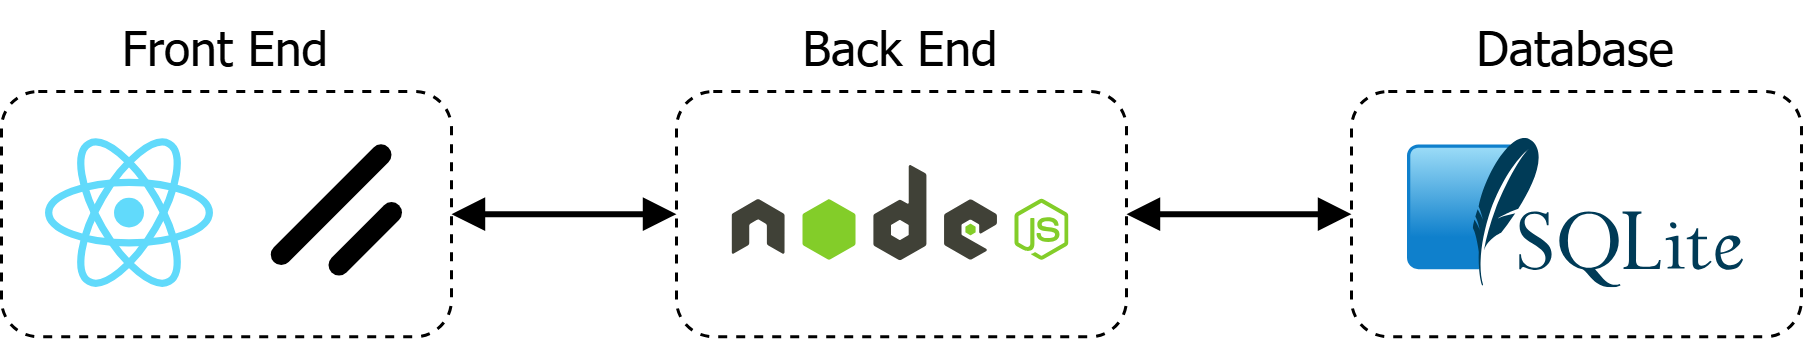
\includegraphics[width=\textwidth]{imgs/ToolsApp.png}
    \caption{Kiến trúc hệ thống CirMetrics}
    \label{fig:chapter6-ToolsApp}
\end{figure}

\subsection{CirMetrics - Demo}
Giao diện của một số tính năng của công cụ CirMetrics được trình bày dưới đây:
\subsubsection{Giao diện thực hiện phân tích mạch}
\begin{figure}[H]
    \centering
    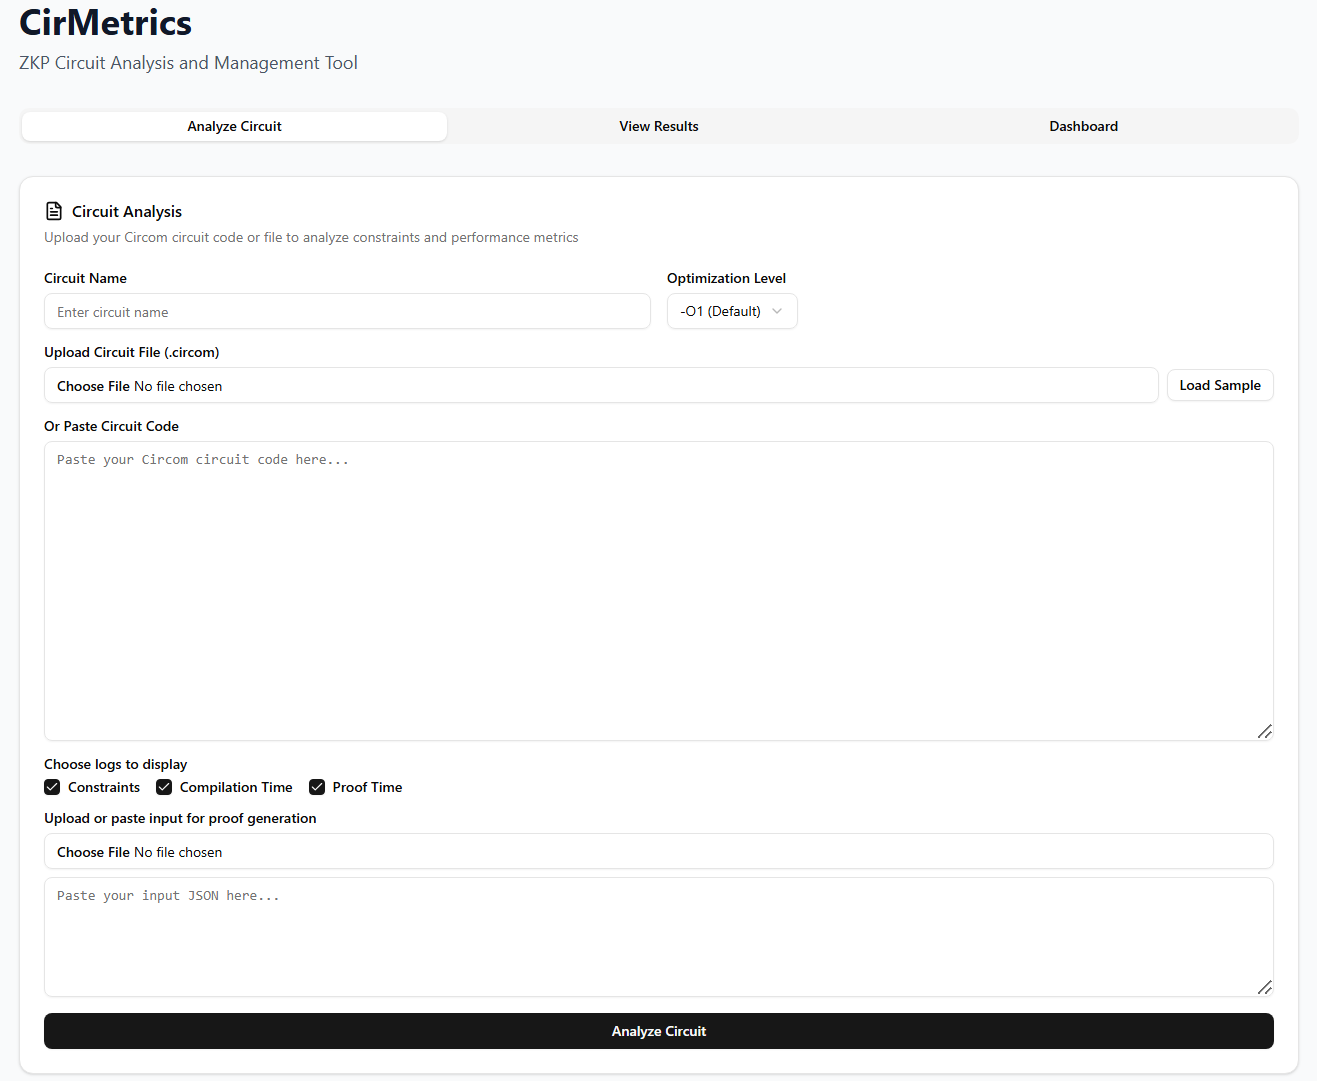
\includegraphics[width=\textwidth]{imgs/analyzescreen.png}
    \caption{Demo chức năng thực hiện phân tích mạch}
    \label{fig:chapter6-analyzescreen}
\end{figure}

Với chức năng phân tích mạch minh hoạ ở hình \ref{fig:chapter6-analyzescreen}, người dùng sẽ nhập tên mạch, sau đó upload file circom hoặc nhập mã nguồn mạch vào khung nhập liệu. Sau đó chọn các chức năng như "constraint" và "compilation time" để biên dịch và hiển thị các thống số của mạch. 

Người dùng cũng có thể chọn thêm "Proof Time" để tạo bằng chứng và nhập thêm đầu vào cho mạch ở dạng JSON để thực hiện tạo ZKP.

\subsubsection{Giao diện xem các kết quả phân tích}
\begin{figure}[H]
    \centering
    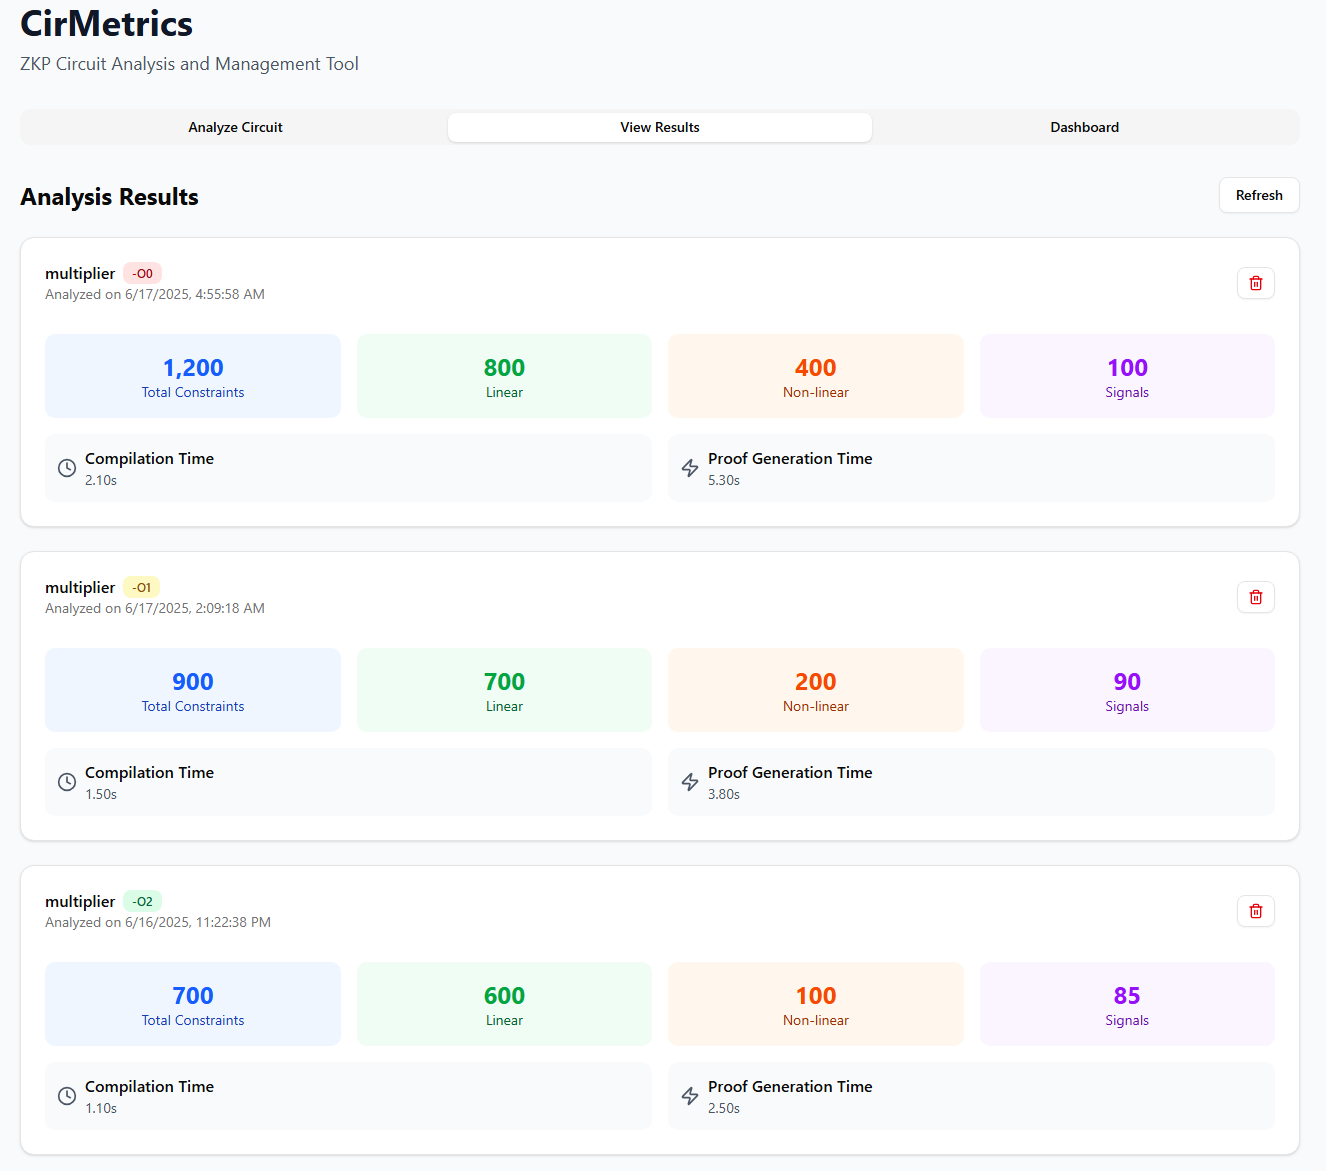
\includegraphics[width=\textwidth]{imgs/resultscreen.png}
    \caption{Demo chức năng xem các kết quả phân tích}
    \label{fig:chapter6-resultscreen}
\end{figure}

Với chức năng xem kết quả phân tích minh hoạ ở hình \ref{fig:chapter6-resultscreen}, người dung có thể xem thống số các mạch đã biên dịch và tạo bằng chứng theo thời gian. Các thông số được hiển thị bao gồm:
\begin{itemize}
    \item Thời gian biên dịch và thời gian tạo bằng chứng
    \item Số lượng ràng buộc (Tổng số lượng ràng buộc, số lượng ràng buộc tuyến tính và ràng buộc không tuyến tính).
    \item Số lượng tín hiệu của mạch.
    \item Thời gian biên dịch mạch.
    \item Thời gian tạo bằng chứng.
\end{itemize}

\subsubsection{Giao diện xem tổng hợp các biểu đồ về các thông số liên quan đến mạch ZK}

\begin{figure}[H]
    \centering
    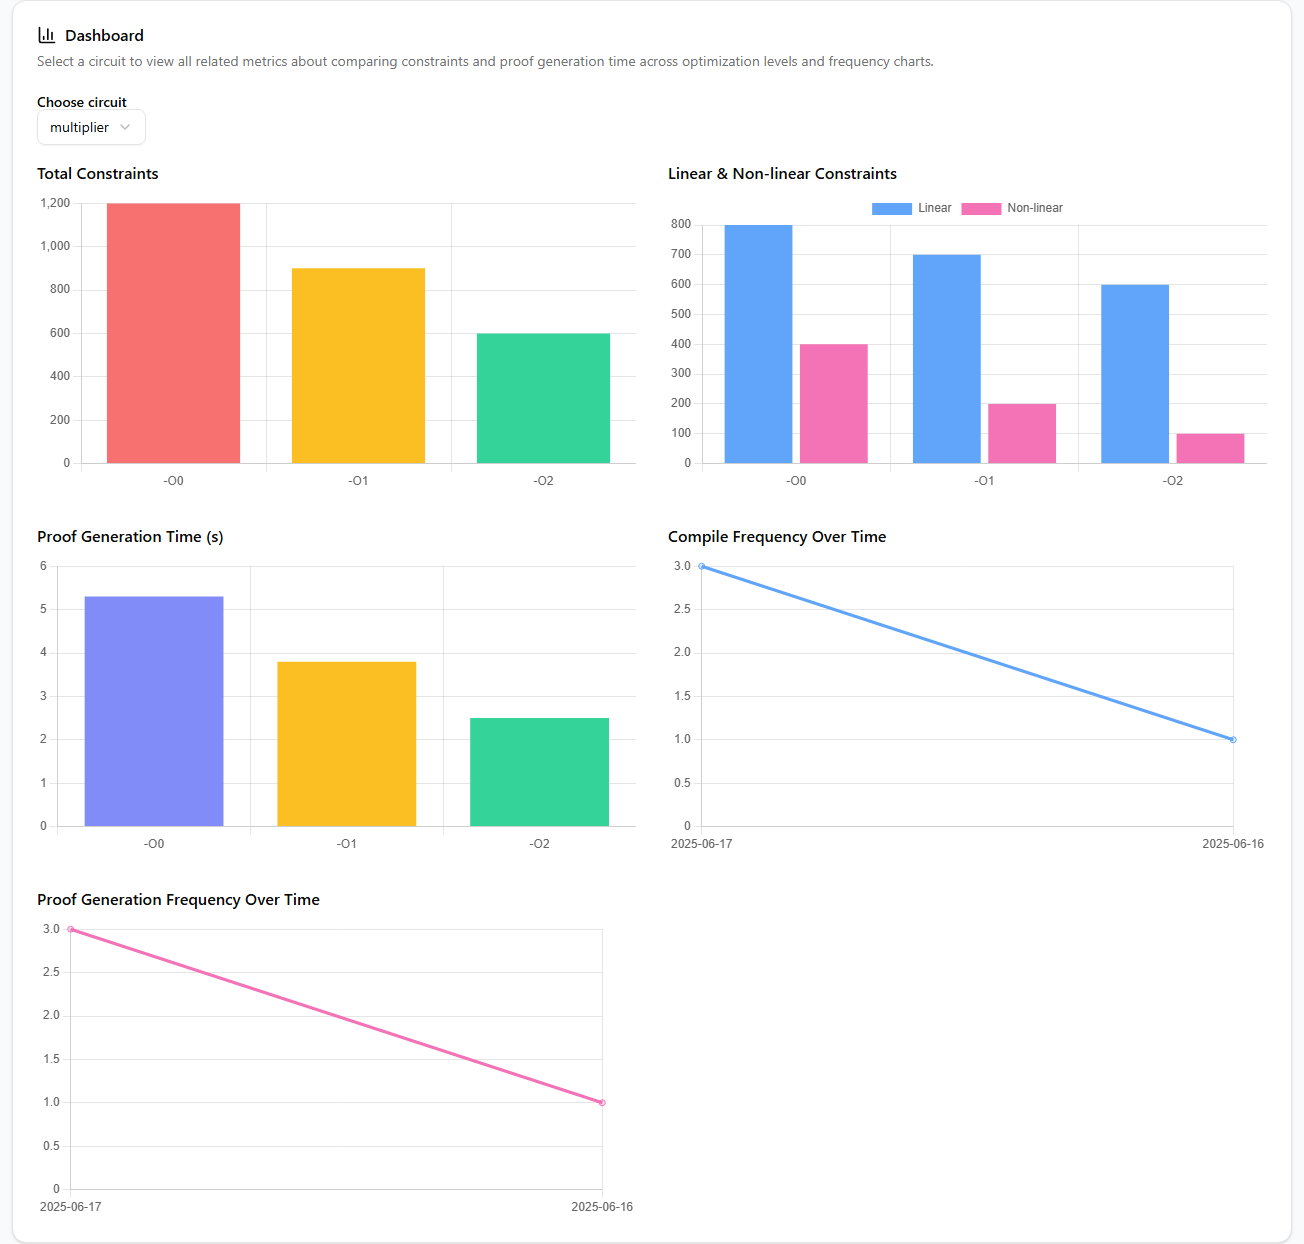
\includegraphics[width=\textwidth]{imgs/dashboardscreen.png}
    \caption{Demo chức năng xem các biểu đồ về các thông số liên quan đến mạch ZK}
    \label{fig:chapter6-dashboardscreen}
\end{figure}

Với chức năng xem các biểu đồ và thông số liên quan đến mạch ZK minh hoạ ở hình \ref{fig:chapter6-dashboardscreen}, người dùng có thể chọn tên mạch và xem các biểu đồ liên quan sau:
\begin{itemize}
    \item Biểu đồ so sánh tổng lượng constraint ở các mức tối ưu mạch khác nhau.
    \item Biểu đồ so sánh tỷ lệ giữa ràng buộc tuyến tính và ràng buộc phi tuyến.
    \item Biểu đồ so sánh thời gian tạo bằng chứng ở các mức tối ưu mạch khác nhau.
    \item Biểu đồ thể hiện tần suất cập nhật mạch và tần suất tạo bằng chứng theo ngày.
\end{itemize}

Với công cụ CirMetrics, các nhà phát triển sẽ thuận tiện hơn trong việc theo dõi trực quan các thông số khi làm việc với mạch ZK. Đồng thời hỗ trợ các nhà phát triển trong việc đưa ra những quyết định hợp lí hơn khi kết hợp công cụ cùng khung \textbf{ZCLS} khi chọn phương án tối ưu hoá mạch phù hợp cho tiến trình phát triển mạch của mình.
\chapter{Kết quả thực nghiệm và đánh giá}
\label{chap:chap5}
\section{Kết quả thực nghiệm}
\begin{figure}[h]
    \centering
    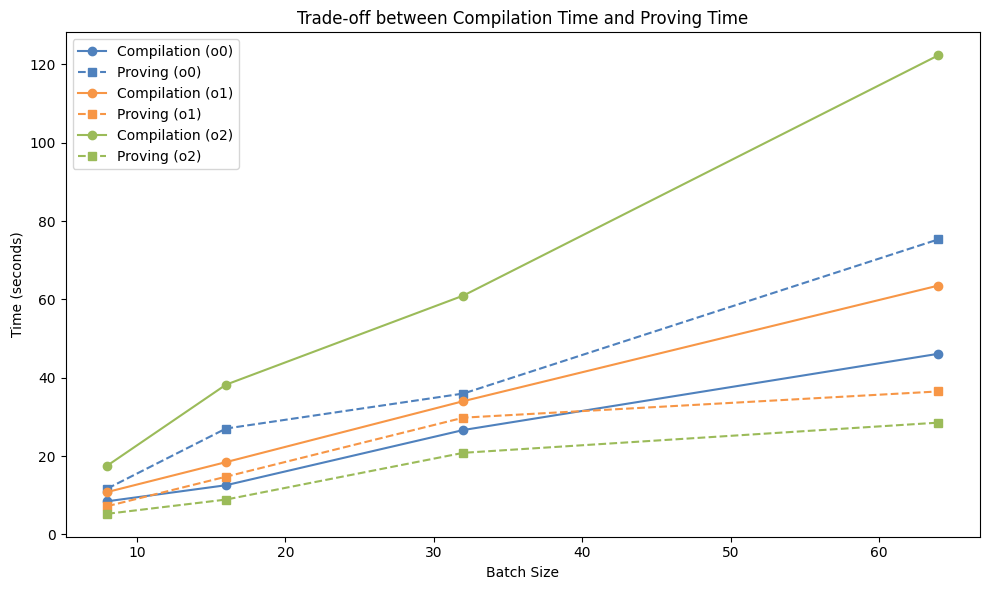
\includegraphics[width=\textwidth]{imgs/compilation_proving_time.png}
    \caption{So sánh thời gian biên dịch mạch và thời gian sinh chứng minh qua các mức tối ưu hóa khác nhau (--O0, --O1, --O2)}
    \label{fig:chapter5-compilation_proving_time}
\end{figure}

Từ Hình \ref{fig:chapter5-compilation_proving_time}, nghiên cứu nhận thấy một sự đánh đổi đáng kể khi áp dụng mức tối ưu hóa cao nhất trong quá trình biên dịch mạch. Cụ thể, thời gian biên dịch cho --O2 gần gấp đôi so với --O1 (165\% ở lô 64 giao dịch). Điều này nhấn mạnh rằng các nhà phát triển phải cân nhắc kỹ lưỡng khi chọn các cờ khác nhau cho các mục tiêu khác nhau trong quá trình phát triển các ứng dụng ZK.

\begin{figure}[H]
    \centering
    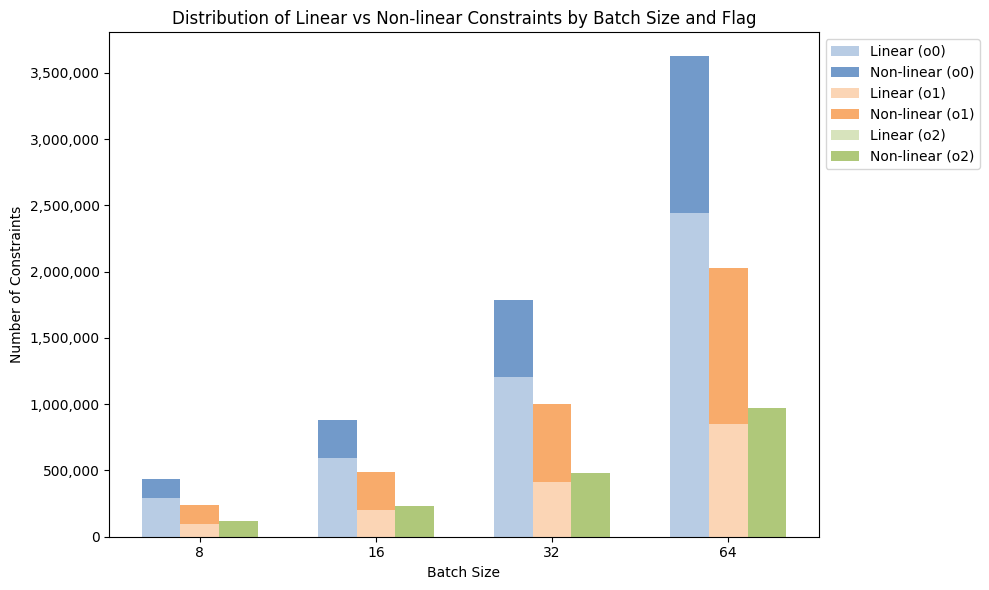
\includegraphics[width=\textwidth]{imgs/constraint_batchsize.png}
    \caption{Phân phối các ràng buộc tuyến tính và phi tuyến theo kích thước lô và cờ tối ưu hóa trình biên dịch.}
    \label{fig:chapter5-constraint_distribution}
\end{figure}

Hình \ref{fig:chapter5-constraint_distribution} cho thấy rằng cả --O1 và --O2 đều tối ưu hóa tốt cho các mạch xác minh theo lô. Việc giảm số lượng ràng buộc tuyến tính thông qua việc sử dụng các cờ tối ưu hóa khác nhau sẽ đóng góp trực tiếp vào hiệu quả của quá trình tạo bằng chứng.


\begin{table}[H]
    \centering
    \caption{Thời gian biên dịch và tạo bằng chứng trung bình cho mỗi tổ hợp kích thước lô và mức tối ưu hóa trình biên dịch.}
    \begin{tabular}{|c|c|c|c|}
        \hline
        \textbf{Kích Thước Lô} & \textbf{Cờ} & \textbf{Thời Gian Biên Dịch (s)} & \textbf{Thời Gian Tạo Bằng Chứng (s)} \\
        \hline
        8   & o0 & 8.458  & 11.696 \\
        8   & o1 & 10.818 & 7.204  \\
        8   & o2 & 17.557 & 5.264  \\
        \hline
        16  & o0 & 12.559 & 27.029 \\
        16  & o1 & 18.455 & 14.735 \\
        16  & o2 & 38.230 & 8.896  \\
        \hline
        32  & o0 & 26.661 & 35.975 \\
        32  & o1 & 34.030 & 29.811 \\
        32  & o2 & 60.991 & 20.838 \\
        \hline
        64  & o0 & 46.124 & 75.341 \\
        64  & o1 & 63.540 & 36.508 \\
        64  & o2 & 122.341 & 28.542 \\
        \hline
    \end{tabular}
    \label{tab:average_performance}
\end{table}

Bảng \ref{tab:average_performance} tóm tắt các chỉ số hiệu suất trung bình cho thời gian biên dịch và thời gian tạo bằng chứng qua các cấu hình khác nhau. Dữ liệu chỉ ra một cách rõ ràng rằng, trong khi --O2 giảm đáng kể số lượng ràng buộc, nó cũng kéo theo thời gian biên dịch cao hơn, nhấn mạnh các sự đánh đổi liên quan đến các chiến lược tối ưu hóa.

\section{Thảo Luận}

    \subsection{Câu hỏi nghiên cứu}
    
    Để làm rõ định hướng khi thực hiện thực nghiệm và phân tích, nghiên cứu này đặt ra hai câu hỏi nghiên cứu sau:
    \begin{itemize}
        \item Các mức tôi ưu hoá ràng buộc đã ảnh hưởng như thế nào đến các mạch ZK phức tạp như mạch xác minh lô giao dịch cho ZK-Rollup?
        % \item Làm thế nào để sử dụng được các mức tối ưu hoá của Circom trong thực tế một cách hiệu quả và nâng cao được hiệu suất của quá trình xây dựng và triển khai ZK-Rollup cũng như các ứng dụng ZK phức tạp khác.
        \item Phương pháp đề xuất \textbf{ZCLS} có góp phần đem lại cải thiện về hiệu suất cho nhà phát triển khi sử dụng các cờ tối ưu hoá của Circom trong quá trình phát triển mạch ZK không? 
        
        \item Khả năng mở rộng và thích ứng của \textbf{ZCLS} với các hệ thống thực tế như thế nào?
    \end{itemize}
    
    \subsection{Phân tích sự ảnh hưởng của các mức tối ưu hoá ràng buộc đối với các độ đo đã ghi nhận}

    Kết quả của các thí nghiệm của nghiên cứu làm nổi bật mối quan hệ phức tạp giữa tối ưu hóa ràng buộc và hiệu suất sinh chứng minh. Đặc biệt, việc sử dụng --O2 có tác động đáng kể đến thiết kế mạch. Bằng cách loại bỏ gần như tất cả các ràng buộc tuyến tính, như được chỉ ra bởi dữ liệu cho thấy các ràng buộc tuyến tính đã giảm xuống bằng không, --O2 tinh giản mạch R1CS, cho phép nó tập trung chủ yếu vào các ràng buộc phi tuyến còn lại. Mặc dù --O2 không giảm đáng kể số lượng ràng buộc phi tuyến, như bảng \ref{tab:average_performance} đã trình bày, số lượng ràng buộc phi tuyến chỉ giảm khoảng 18\% ở kích thước lô 64 so với --O0; nhưng --O2 đã thể hiện hiệu quả trong việc loại bỏ các ràng buộc tuyến tính, vốn không làm thay đổi cấu trúc logic của mạch Groth16. Sự tối ưu hóa này cho phép người chứng minh tập trung vào các ràng buộc phi tuyến, điều này rất quan trọng để duy trì tính toàn vẹn của quá trình sinh chứng minh.

    Bên cạnh đó, các kết quả thực nghiệm của nghiên cứu cho thấy phí gas cho việc xác minh vẫn ổn định qua các kích thước lô và số lượng ràng buộc khác nhau. Sự ổn định này có thể được giải thích bởi cho kiến trúc của Groth16, trong đó số lượng các phần tử trong bằng chứng cần được xác minh là cố định, bao gồm ba phần tử trên một đường cong elliptic \cite{groth2016size}. Ngoài ra, các đầu vào công khai, chẳng hạn như gốc (root) giao dịch, tương đối nhỏ và không ảnh hưởng đáng kể đến tổng chi phí gas.

    Tương tự, kích thước chứng minh rất ổn định nhờ vào cấu trúc cố định của nó, chỉ bao gồm ba phần tử trên đường cong elliptic. Đặc điểm này nhấn mạnh rằng trong khi tổng số lượng ràng buộc có thể thay đổi, kích thước chứng minh không dao động đáng kể với những thay đổi này.

    Trong bối cảnh ZK-Rollup và các giao dịch ERC-20, các hoạt động mật mã tiêu chuẩn như xác minh chữ ký và hàm băm tạo sẽ ra một số lượng lớn các ràng buộc phi tuyến. Thêm vào đó, các hoạt động logic trừu tượng hơn, chẳng hạn như quản lý và xác minh các chứng minh Merkle, cũng sử dụng các hoạt động mật mã này, dẫn đến việc sinh ra một khối lượng lớn các ràng buộc phi tuyến cho mạch ZK. Việc sử dụng --O2 hiệu quả trong việc cô đọng các ràng buộc chỉ còn những ràng buộc thiết yếu, từ đó tối ưu hóa quá trình sinh chứng minh.
    
    % \item \textbf{Phân tích về thời gian biên dịch của --O2}
    
    % Như đã đề cập trong Chương \ref{chap:chap3}, cờ tối ưu hóa --O2 của trình biên dịch Circom áp dụng các kỹ thuật nâng cao để giảm thiểu số lượng ràng buộc trong mạch R1CS, đặc biệt là sử dụng thuật toán khử Gauss dạng lười (Lazy Form of Gaussian Elimination). Mặc dù --O2 mang lại hiệu quả vượt trội trong việc giảm ràng buộc và tăng tốc độ tạo bằng chứng, quá trình biên dịch ở mức này lại tốn nhiều thời gian và tài nguyên tính toán hơn đáng kể so với -O0 và -O1. Điều này có thể được giải thích chi tiết hơn dựa trên cơ chế hoạt động nội bộ của trình biên dịch Circom và sự khác biệt trong các bước tiền xử lý so với -O1.

    \subsection{Kịch bản thử nghiệm kiểm tra ảnh hưởng của ZCLS với hiệu suất của việc phát triển ZK-Rollup}

    Các kịch bản này sử dụng dữ liệu thực nghiệm đã thu thập để mô phỏng hiệu quả của ZCLS trong
    các tình huống giả định thực tế:
    
\begin{enumerate}
    \item \textbf{Kịch bản 1: Giai đoạn gỡ lỗi chuyên sâu (Intensive Debugging Phase)}

    \begin{itemize}
    \item \textbf{Mô tả:} Một nhà phát triển đang trong giai đoạn gỡ lỗi một mạch ZK phức tạp với kích thước lô là 64. Trong một ngày làm việc, họ cần thực hiện 100 lần thay đổi nhỏ và biên dịch lại mạch để kiểm tra lỗi. Khối lượng tạo bằng chứng trong mỗi lần kiểm tra là rất thấp để kiểm tra tính chính xác của bằng chứng cơ bản.

    \item\textbf{Mục tiêu:} Giảm tối đa tổng thời gian chờ đợi biên dịch để duy trì chu kỳ phản hồi nhanh.

    \item\textbf{Phân tích theo ZCLS sử dụng dữ liệu thực nghiệm:}
    \begin{itemize}
    \item Trong trường hợp "Tần suất cập nhật mạch Rất Cao" và "Khối lượng tạo bằng chứng Rất Thấp", cờ --O0 được khuyến nghị.
    \item Thời gian biên dịch trung bình của --O0: 46.124 giây.
    \item Thời gian biên dịch trung bình của --O1: 63.540 giây.
    \item Thời gian biên dịch trung bình của --O2: 122.341 giây.
    \end{itemize}

    \item\textbf{Kết quả:}
    \begin{itemize}
    \item Sử dụng --O0: Tổng thời gian biên dịch = 100 lần * 46.124 giây/lần = 4612.4 giây (khoảng 76.87 phút).
    \item Sử dụng --O1: Tổng thời gian biên dịch = 100 lần * 63.540 giây/lần = 6354 giây (khoảng 105.9 phút).
    \item Sử dụng --O2: Tổng thời gian biên dịch = 100 lần * 122.341 giây/lần = 12234.1 giây (khoảng 203.9 phút).
    \end{itemize}

    \item\textbf{Lợi ích đem lại:} Trong kịch bản này, việc tuân thủ ZCLS và sử dụng --O0 giúp nhà phát triển tiết kiệm được khoảng 29 phút (giảm khoảng 27.4\% thời gian) so với --O1 và 127 phút (giảm khoảng 62.3\% thời gian) so với --O2 trong mỗi ngày gỡ lỗi. Điều này giúp duy trì năng suất cao và giảm sự gián đoạn trong quá trình làm việc.

\end{itemize}

\item \textbf{Kịch bản 2: Triển khai thực tế với khối lượng giao dịch lớn (Production Deployment with High Transaction Volume)}

\begin{itemize}
\item\textbf{Mô tả:} Một ZK-Rollup đã được triển khai và đang xử lý hàng chục nghìn giao dịch mỗi ngày. Mạch ZK đã ổn định và tần suất cập nhật mạch là rất thấp. Mục tiêu chính là tối thiểu hóa thời gian tạo bằng chứng để đạt được thông lượng cao và giảm chi phí vận hành.

\item\textbf{Mục tiêu:} Giảm tối đa thời gian tạo bằng chứng để tối đa hóa thông lượng và hiệu quả chi phí.

\item\textbf{Phân tích theo ZCLS với dữ liệu thực nghiệm:}
\begin{itemize}
    \item Trong trường hợp "Tần suất cập nhật mạch Thấp" và "Khối lượng tạo bằng chứng Cao", cờ --O2 được khuyến nghị.
    \item Thời gian tạo bằng chứng trung bình của --O0: 75.341 giây.
    \item Thời gian tạo bằng chứng trung bình của --O1: 36.508 giây.
    \item Thời gian tạo bằng chứng trung bình của --O2: 28.542 giây.
\end{itemize}

\item\textbf{Kết quả:}
\begin{itemize}
    \item Giả sử hệ thống cần tạo 1000 bằng chứng mỗi ngày.
    \item Sử dụng --O0: Tổng thời gian tạo bằng chứng = 1000 * 75.341 giây = 75341 giây (khoảng 20.9 giờ).
    \item Sử dụng --O1: Tổng thời gian tạo bằng chứng = 1000 * 36.508 giây = 36508 giây (khoảng 10.1 giờ).
    \item Sử dụng --O2: Tổng thời gian tạo bằng chứng = 1000 * 28.542 giây = 28542 giây (khoảng 7.9 giờ).
\end{itemize}

\item\textbf{Lợi ích đem lại:} Việc tuân thủ ZCLS và sử dụng --O2 giúp giảm đáng kể tổng thời gian tạo bằng chứng, từ đó tăng thông lượng giao dịch và cải thiện hiệu suất ZK-Rollup. So với --O0, --O2 giúp tiết kiệm khoảng 13 giờ thời gian tạo bằng chứng cho 1000 bằng chứng, và so với --O1 là 2.2 giờ. Điều này trực tiếp chuyển thành thông lượng cao hơn và khả năng mở rộng tốt hơn cho ZK-Rollup.
\end{itemize}

    \end{enumerate}
%     Các phát hiện cũng nhấn mạnh rằng thời gian biên dịch là một rào cản phát triển đáng kể cho các triển khai ZK-Rollup quy mô lớn. Mặc dù cần thiết phải sử dụng --O2 để đảm bảo sinh chứng minh hiệu quả, sự đánh đổi với thời gian biên dịch tăng lên có thể làm gián đoạn quy trình làm việc khi phát triển ứng dụng. Điều này cần một cách tiếp cận phát triển hai giai đoạn: trong các giai đoạn xây dựng và thử nghiệm, các nhà phát triển nên sử dụng --O1 làm mặc định để tối ưu hóa hiệu quả quy trình làm việc, trong khi chuyển sang --O2 cho sản xuất để tối đa hóa hiệu quả tạo bằng chứng.

%     Để hướng dẫn các nhà phát triển trong việc lựa chọn cờ tối ưu hóa, chúng tôi đề xuất một khung, như được trình bày trong Bảng \ref{tab:optimization_flag_selection} và Hình \ref{fig:chapter5-framework}, dựa trên tần suất cập nhật mạch và khối lượng chứng minh cần được sinh ra:

% \begin{itemize}
%     \item \textbf{Tần Suất Cập Nhật Mạch Cao:} Ưu tiên thời gian biên dịch nhanh để tăng tốc phát triển và giảm thời gian chờ cho các sửa đổi mạch.
%     \item \textbf{Tần Suất Cập Nhật Mạch Thấp:} Ưu tiên thời gian sinh chứng minh thấp, vì mạch sẽ được sử dụng để sinh nhiều chứng minh trong các hoạt động thực tế.
%     \item \textbf{Khối Lượng Sinh Chứng Minh Lớn:} Tối ưu hóa để giảm tổng thời gian sinh chứng minh.
%     \item \textbf{Khối Lượng Sinh Chứng Minh Nhỏ:} Chấp nhận thời gian chứng minh cao hơn để đổi lấy thời gian biên dịch nhanh hơn.
% \end{itemize}

% \begin{table}[h]
%     \centering
%     \caption{Các mức tối ưu hóa trình biên dịch Circom được khuyến nghị dựa trên giai đoạn phát triển, tần suất cập nhật mạch và khối lượng bằng chứng được tạo.}
%     \resizebox{\textwidth}{!}{%
%     \begin{tabular}{|l|l|l|l|}
%         \hline
%         \textbf{Giai Đoạn Phát Triển} & \textbf{Tần Suất Cập Nhật Mạch} & \textbf{Khối Lượng Tạo Bằng Chứng} & \textbf{Cờ Được Khuyến Nghị} \\
%         \hline
%         Phát Triển, Thử Nghiệm & Cao & Thấp & --O1 \\
%         Phát Triển, Thử Nghiệm & Cao & Cao & --O1 \\
%         Triển Khai Thực Tế & Thấp & Cao & --O2 \\
%         Triển Khai Thực Tế & Thấp & Thấp & --O2 \\
%         Trường Hợp Đặc Biệt (Gỡ Lỗi) & Rất Cao (Thường Xuyên) & Rất Thấp & --O0 \\
%         \hline
%     \end{tabular}
%     }
%     \label{tab:optimization_flag_selection}
% \end{table}

% \begin{figure}[h] % 'h' để đặt ảnh gần vị trí lệnh
%     \centering % Căn giữa ảnh
%     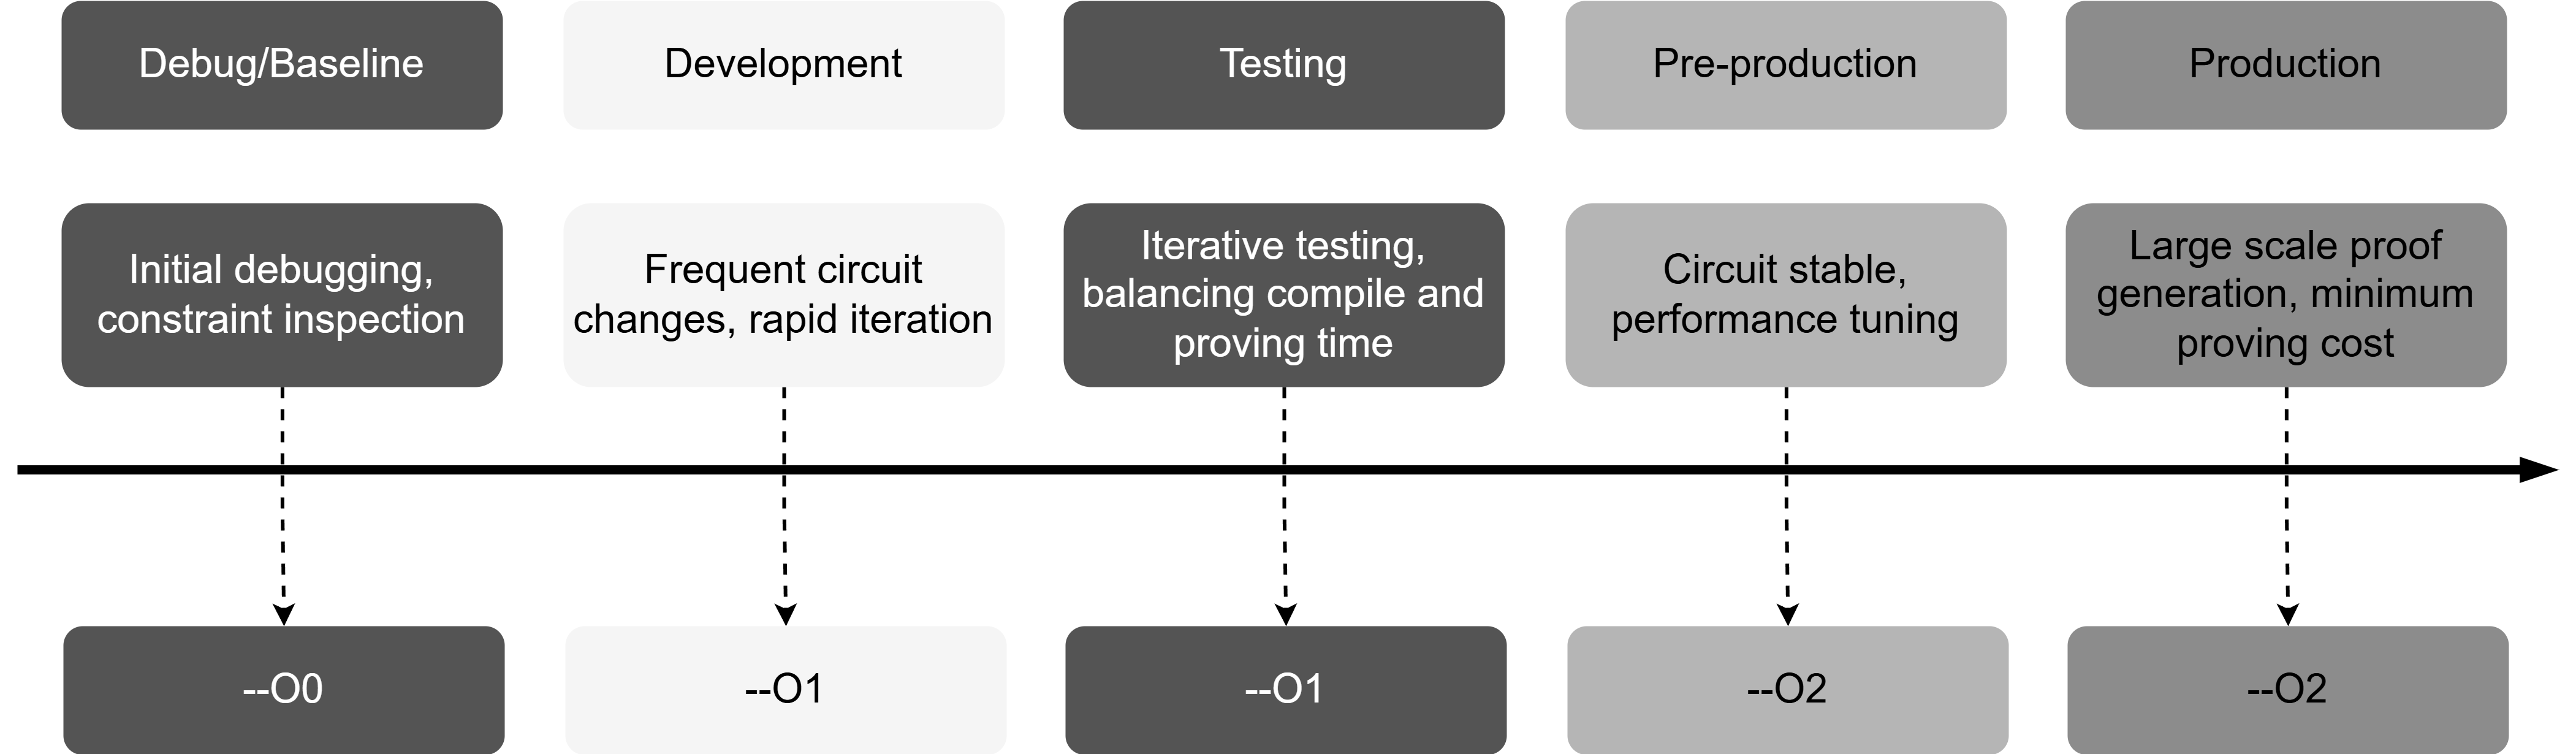
\includegraphics[width=\textwidth]{imgs/framework.png}
%     \caption{Khung chọn cờ tối ưu hóa trình biên dịch Circom dựa trên giai đoạn phát triển, tần suất cập nhật mạch và khối lượng tạo bằng chứng}
%     \label{fig:chapter5-framework}
% \end{figure}

    \subsection{Khả năng mở rộng và thích ứng của ZCLS với các hệ thống thực tế}

    Nghiên cứu này nhận thức rằng các thử nghiệm hiện tại được thực hiện với kích thước lô tối đa là 64. Trong thực tế, các hệ thống ZK-Rollup có thể xử lý các lô giao dịch lên đến vài nghìn hoặc thậm chí hàng chục nghìn, dẫn đến số lượng ràng buộc và thời gian biên dịch/tạo bằng chứng sẽ tăng lên đáng kể. Do đó, các giá trị được dùng trong phần giải thích khung cần được hiểu là dựa trên dữ liệu trong phạm vi thử nghiệm của nghiên cứu.

    Tuy nhiên, \textbf{nguyên lý cốt lõi và xu hướng} về sự đánh đổi giữa thời gian biên dịch và thời gian tạo bằng chứng giữa các cờ tối ưu hóa (--O0, --O1, --O2) vẫn sẽ được duy trì ngay cả ở quy mô lớn hơn. Cụ thể:

    \begin{itemize}
    \item --O0 sẽ là lựa chọn nhanh nhất về biên dịch nhưng chậm nhất về tạo bằng chứng.
    \item --O2 sẽ là lựa chọn chậm nhất về biên dịch nhưng nhanh nhất về tạo bằng chứng.
    \item --O1 sẽ cung cấp sự cân bằng hợp lý giữa hai yếu tố này.
    \end{itemize}

    % Tuy nhiên, nguyên lý cốt lõi và xu hướng về sự đánh đổi giữa thời gian biên dịch và thời gian tạo bằng chứng giữa các mức cờ tối ưu hóa (–O0, –O1, –O2) vẫn được duy trì ngay cả khi mở rộng quy mô. Cụ thể, cờ –O0 cho phép thời gian biên dịch nhanh nhất nhưng dẫn đến thời gian tạo bằng chứng chậm nhất. Ngược lại, cờ –O2 đòi hỏi thời gian biên dịch dài hơn song mang lại hiệu quả cao nhất trong việc rút ngắn thời gian tạo bằng chứng. Trong khi đó, cờ –O1 đóng vai trò trung gian, cung cấp sự cân bằng hợp lý giữa hai yếu tố trên.
    
    Khung này sẽ cung cấp một cách tiếp cận có cấu trúc giúp các nhà phát triển đưa ra quyết định thông minh về các cờ tối ưu hóa trong Circom, đảm bảo rằng chiến lược được chọn phù hợp với các yêu cầu cụ thể của giai đoạn phát triển ứng dụng.

    Bằng cách cung cấp dữ liệu thực nghiệm và một khung đề xuất để chọn các cờ tối ưu, nghiên cứu này mở rộng hơn các thảo luận lý thuyết về hiệu suất ZKP, cung cấp hướng dẫn thực tiễn cho việc phát triển các ứng dụng phi tập trung (DApps) và ứng dụng ZK trong các tình huống thực tế. Khung tối ưu hóa được đề xuất cho phép các nhà phát triển kiểm soát độ phức tạp của việc sinh ZKP, giảm thiểu thời gian thử nghiệm và sai sót, và tăng tốc độ triển khai ứng dụng.




\chapter{Kết luận và hướng phát triển}
\label{chap:chap6}
\section{Kết luận}
Nghiên cứu này đã thực hiện một phân tích thực nghiệm toàn diện về tác động của các cờ tối ưu hóa trình biên dịch Circom (–O0, –O1, –O2) lên hiệu suất của hệ thống ZK-Rollup xử lý giao dịch ERC-20, sử dụng backend Groth16. Thông qua việc mô phỏng và đánh giá các chỉ số quan trọng như số lượng ràng buộc, thời gian biên dịch mạch, và thời gian tạo bằng chứng, nghiên cứ đã làm rõ những đánh đổi hiệu suất liên quan đến từng mức độ tối ưu hóa.

Kết quả cho thấy cờ tối ưu hóa –O2, mặc dù làm tăng đáng kể thời gian biên dịch mạch, lại mang lại hiệu quả vượt trội trong việc giảm số lượng ràng buộc và rút ngắn đáng kể thời gian tạo bằng chứng. Điều này khẳng định giá trị của việc tối ưu hóa sâu ở cấp độ ràng buộc đối với hiệu suất của quá trình tạo bằng chứng, vốn là một nút thắt quan trọng trong các hệ thống ZKP. Ngược lại, cờ –O1 cung cấp một sự cân bằng hợp lý, giảm khoảng 56\% ràng buộc so với –O0 mà không gây ra chi phí biên dịch quá lớn, cho thấy đây là lựa chọn phù hợp cho giai đoạn
phát triển và kiểm thử lặp lại. 

Nghiên cứu cũng tái khẳng định rằng, đối với Groth16, kích thước bằng chứng và thời gian xác minh bằng chứng là ổn định và không phụ thuộc vào số lượng ràng buộc, trong khi thời gian tạo bằng chứng chịu ảnh hưởng trực tiếp từ số lượng và bản chất của các ràng buộc. 

Dựa trên những phân tích định lượng này, nghiên cứu đã đề xuất khung lựa chọn cờ tối ưu hóa thực tiễn \textbf{ZCLS}, giúp các nhà phát triển đưa ra quyết định đúng đắn dựa trên giai đoạn phát triển dự án, tần suất cập nhật mạch và khối lượng bằng chứng cần tạo. Khung này không chỉ tối ưu hóa việc sử dụng tài nguyên mà còn góp phần đẩy nhanh quá trình phát triển và triển khai các ứng dụng sử dụng ZKP thức trong thực tế.

Nghiên cứu này đã cung cấp dữ liệu thực nghiệm chi tiết có giá trị sử dụng làm cơ sở xác thực cho các dự đoán lý thuyết liên quan đến tối ưu hóa hệ ràng buộc, cùng với một phương pháp luận có cấu trúc để hiểu rõ hơn về cơ chế hoạt động của các tùy chọn tối ưu hóa trong Circom. Điều này không chỉ có thể hỗ trợ các nhà phát triển tiết kiệm thời gian và tài nguyên khi phát triển và triển khai các ứng dụng ZK-Rollup mà còn hỗ trợ việc áp dụng rộng rãi công nghệ chứng minh không kiến thức trong các hệ thống blockchain và các ứng dụng khác đòi hỏi tính bảo mật và hiệu suất cao.

Tuy đã nỗ lực để đạt được các mục tiêu nghiên cứu đã đề ra và cung cấp những phân tích định lượng chi tiết về tác động của các cờ tối ưu hóa trong trình biên dịch Circom, nghiên cứu của em vẫn còn một số hạn chế nhất định. Các thử nghiệm được thực hiện trên hệ thống AMD Ryzen 8 nhân, 16 luồng với 32GB RAM, đảm bảo tính nhất quán nhưng có thể cho kết quả khác biệt trên các kiến trúc phần cứng hoặc môi trường phức tạp hơn. Mạch ERC-20 mô phỏng được chọn làm trường hợp nghiên cứu tuy đủ phức tạp để đánh giá tối ưu hóa ràng buộc, nhưng chưa phản ánh đầy đủ sự đa dạng của các hệ thống ZK-Rollup thực tế với nhiều loại giao dịch và hợp đồng thông minh phức tạp. Kết quả thực nghiệm trên các lô nhỏ ($\leq$ 64) không thể dự đoán chính xác hành vi với hàng ngàn giao dịch. Tuy nhiên, kết quả này cung cấp một cái nhìn tổng quan về xu hướng và cơ chế tối ưu hóa, là bước đầu để hiểu hành vi ở quy mô lớn hơn. Ngoài ra, phạm vi nghiên cứu giới hạn ở trình biên dịch Circom và hệ thống zk-SNARK Groth16, chưa so sánh với các hệ thống ZKP khác ví dụ như Plonk. Dù vậy, việc tập trung vào một bộ công cụ cụ thể đã cho phép nghiên cứu phân tích chi tiết hơn, mang lại những hiểu biết quan trọng về tối ưu hóa ràng buộc, đồng thời đây cũng sẽ là nền tảng cho nhiều hướng nghiên cứu tiếp theo.

% Nghiên cứu tập trung chủ yếu vào thời gian biên dịch và tạo bằng chứng, nhưng chưa đi sâu vào phân tích định lượng chi phí bộ nhớ và CPU.

\section{Hướng phát triển}
Để tiếp tục phát triển và mở rộng nghiên cứu này, em đề xuất một số hướng tiềm năng sau:

\begin{itemize}
    \item So sánh với các trình biên dịch ZKP khác: Mở rộng nghiên cứu để so sánh khả năng tối ưu hóa ràng buộc và hiệu suất tổng thể giữa Circom và các trình biên dịch ZKP khác như ZoKrates, Noir, hoặc các framework dựa trên Rust/Halo2. Điều này sẽ cung cấp một cái nhìn toàn diện hơn về bức tranh tối ưu hóa ZKP và giúp các nhà phát triển lựa chọn công cụ phù hợp nhất cho nhu cầu của họ.
    \item Nghiên cứu các kỹ thuật tối ưu hóa mạch nâng cao: Nghiên cứu và thử nghiệm các kỹ thuật tối ưu hóa mạch ZKP ở cấp độ thiết kế mạch, không chỉ giới hạn ở các cờ tối ưu hóa của trình biên dịch. Điều này có thể bao gồm việc sử dụng các cấu trúc dữ liệu hiệu quả hơn, tối ưu hóa các phép toán mật mã cốt lõi, hoặc cải tiến thuật toán tối ưu hoá ràng buộc.
    \item Đánh giá trên các loại giao dịch và ứng dụng khác: Mở rộng phạm vi thực nghiệm để bao gồm các loại giao dịch phức tạp hơn (ví dụ: giao dịch DeFi, NFT minting) hoặc các ứng dụng ZK-Rollup khác ngoài chuyển token ERC-20. Điều này sẽ giúp đánh giá tính tổng quát và khả năng áp dụng của các kết quả tối ưu hóa.
    \item Phân tích tác động của phần cứng: Nghiên cứu sâu hơn về tác động của cấu hình phần cứng (CPU, GPU, bộ nhớ) lên thời gian biên dịch và tạo bằng chứng ở các mức tối ưu hóa khác nhau. Điều này sẽ cung cấp cái nhìn chi tiết hơn về yêu cầu tài nguyên và giúp tối ưu hóa việc triển khai trong môi trường sản xuất.
    \item Phát triển công cụ tự động hóa và tích hợp: Phát triển thêm tính năng cho \textbf{CirMetrics} hỗ trợ để tự động hóa quá trình lựa chọn cờ tối ưu ràng buộc dựa trên các tham số đầu vào của mạch và mục tiêu hiệu suất mong muốn. Mục tiêu là để giúp các nhà phát triển dễ dàng áp dụng các khuyến nghị được đề xuất.
\end{itemize}

Những hướng phát triển này không chỉ giúp làm sâu sắc thêm hiểu biết về tối ưu hóa ZKP mà còn góp phần vào việc xây dựng các hệ thống zk-rollup mạnh mẽ, hiệu quả và dễ dàng hơn trong tương lai.

%\include{chapters/main/chapter7.tex}

% Appendix chapter in thesis
%include{chapters/back/MAPR2024_LongHoangNguyen/apendixA}

% Print references
 \printbibliography[heading=bibintoc, title = {Tài liệu tham khảo}]

\appendix

\includepdf[page={1-6}]{ICCAE2026.pdf}

\includepdf[page={1-17}]{IEEEAccess.pdf}
\end{document}
